%%*************************************************************************
% RELab LaTeX template - this template is based on the IEEE template
%%*************************************************************************

%% bare_conf.tex
%% V1.4b
%% 2015/08/26
%% by Michael Shell
%% See:
%% http://www.michaelshell.org/
%% for current contact information.
%%
%% This is a skeleton file demonstrating the use of IEEEtran.cls
%% (requires IEEEtran.cls version 1.8b or later) with an IEEE
%% conference paper.
%%
%% Support sites:
%% http://www.michaelshell.org/tex/ieeetran/
%% http://www.ctan.org/pkg/ieeetran
%% and
%% http://www.ieee.org/

%%*************************************************************************
%% Legal Notice:
%% This code is offered as-is without any warranty either expressed or
%% implied; without even the implied warranty of MERCHANTABILITY or
%% FITNESS FOR A PARTICULAR PURPOSE! 
%% User assumes all risk.
%% In no event shall the IEEE or any contributor to this code be liable for
%% any damages or losses, including, but not limited to, incidental,
%% consequential, or any other damages, resulting from the use or misuse
%% of any information contained here.
%%
%% All comments are the opinions of their respective authors and are not
%% necessarily endorsed by the IEEE.
%%
%% This work is distributed under the LaTeX Project Public License (LPPL)
%% ( http://www.latex-project.org/ ) version 1.3, and may be freely used,
%% distributed and modified. A copy of the LPPL, version 1.3, is included
%% in the base LaTeX documentation of all distributions of LaTeX released
%% 2003/12/01 or later.
%% Retain all contribution notices and credits.
%% ** Modified files should be clearly indicated as such, including  **
%% ** renaming them and changing author support contact information. **
%%*************************************************************************

% *** Authors should verify (and, if needed, correct) their LaTeX system  ***
% *** with the testflow diagnostic prior to trusting their LaTeX platform ***
% *** with production work. The IEEE's font choices and paper sizes can   ***
% *** trigger bugs that do not appear when using other class files.       ***
% The testflow support page is at:
% http://www.michaelshell.org/tex/testflow/


\documentclass[conference,a4paper]{IEEEtran}
% Some Computer Society conferences also require the compsoc mode option,
% but others use the standard conference format.
%
% If IEEEtran.cls has not been installed into the LaTeX system files,
% manually specify the path to it like:
% \documentclass[conference]{../sty/IEEEtran}

% Some very useful LaTeX packages include:
% (uncomment the ones you want to load)


% *** MISC UTILITY PACKAGES ***
%
%\usepackage{ifpdf}
\usepackage{todonotes}

% Heiko Oberdiek's ifpdf.sty is very useful if you need conditional
% compilation based on whether the output is pdf or dvi.
% usage:
% \ifpdf
%   % pdf code
% \else
%   % dvi code
% \fi
% The latest version of ifpdf.sty can be obtained from:
% http://www.ctan.org/pkg/ifpdf
% Also, note that IEEEtran.cls V1.7 and later provides a builtin
% \ifCLASSINFOpdf conditional that works the same way.
% When switching from latex to pdflatex and vice-versa, the compiler may
% have to be run twice to clear warning/error messages.


% *** CITATION PACKAGES ***
%
%\usepackage{cite}
% cite.sty was written by Donald Arseneau
% V1.6 and later of IEEEtran pre-defines the format of the cite.sty package
% \cite{} output to follow that of the IEEE. Loading the cite package will
% result in citation numbers being automatically sorted and properly
% "compressed/ranged". e.g., [1], [9], [2], [7], [5], [6] without using
% cite.sty will become [1], [2], [5]--[7], [9] using cite.sty. cite.sty's
% \cite will automatically add leading space, if needed. Use cite.sty's
% noadjust option (cite.sty V3.8 and later) if you want to turn this off
% such as if a citation ever needs to be enclosed in parenthesis.
% cite.sty is already installed on most LaTeX systems. Be sure and use
% version 5.0 (2009-03-20) and later if using hyperref.sty.
% The latest version can be obtained at:
% http://www.ctan.org/pkg/cite
% The documentation is contained in the cite.sty file itself.


% *** GRAPHICS RELATED PACKAGES ***
%
\ifCLASSINFOpdf
   \usepackage[pdftex]{graphicx}
  % declare the path(s) where your graphic files are
  % \graphicspath{{../pdf/}{../jpeg/}}
  % and their extensions so you won't have to specify these with
  % every instance of \includegraphics
  % \DeclareGraphicsExtensions{.pdf,.jpeg,.png}
%\else
  % or other class option (dvipsone, dvipdf, if not using dvips). graphicx
  % will default to the driver specified in the system graphics.cfg if no
  % driver is specified.
  % \usepackage[dvips]{graphicx}
  % declare the path(s) where your graphic files are
  % \graphicspath{{../eps/}}
  % and their extensions so you won't have to specify these with
  % every instance of \includegraphics
  % \DeclareGraphicsExtensions{.eps}
%\fi
% graphicx was written by David Carlisle and Sebastian Rahtz. It is
% required if you want graphics, photos, etc. graphicx.sty is already
% installed on most LaTeX systems. The latest version and documentation
% can be obtained at: 
% http://www.ctan.org/pkg/graphicx
% Another good source of documentation is "Using Imported Graphics in
% LaTeX2e" by Keith Reckdahl which can be found at:
% http://www.ctan.org/pkg/epslatex
%
% latex, and pdflatex in dvi mode, support graphics in encapsulated
% postscript (.eps) format. pdflatex in pdf mode supports graphics
% in .pdf, .jpeg, .png and .mps (metapost) formats. Users should ensure
% that all non-photo figures use a vector format (.eps, .pdf, .mps) and
% not a bitmapped formats (.jpeg, .png). The IEEE frowns on bitmapped formats
% which can result in "jaggedy"/blurry rendering of lines and letters as
% well as large increases in file sizes.
%
% You can find documentation about the pdfTeX application at:
% http://www.tug.org/applications/pdftex


% *** MATH PACKAGES ***
%
\usepackage{amsmath}
% A popular package from the American Mathematical Society that provides
% many useful and powerful commands for dealing with mathematics.
%
% Note that the amsmath package sets \interdisplaylinepenalty to 10000
% thus preventing page breaks from occurring within multiline equations. Use:
\interdisplaylinepenalty=2500
% after loading amsmath to restore such page breaks as IEEEtran.cls normally
% does. amsmath.sty is already installed on most LaTeX systems. The latest
% version and documentation can be obtained at:
% http://www.ctan.org/pkg/amsmath


% *** SPECIALIZED LIST PACKAGES ***
%
%\usepackage{algorithmic}
% algorithmic.sty was written by Peter Williams and Rogerio Brito.
% This package provides an algorithmic environment fo describing algorithms.
% You can use the algorithmic environment in-text or within a figure
% environment to provide for a floating algorithm. Do NOT use the algorithm
% floating environment provided by algorithm.sty (by the same authors) or
% algorithm2e.sty (by Christophe Fiorio) as the IEEE does not use dedicated
% algorithm float types and packages that provide these will not provide
% correct IEEE style captions. The latest version and documentation of
% algorithmic.sty can be obtained at:
% http://www.ctan.org/pkg/algorithms
% Also of interest may be the (relatively newer and more customizable)
% algorithmicx.sty package by Szasz Janos:
% http://www.ctan.org/pkg/algorithmicx


% *** ALIGNMENT PACKAGES ***
%
%\usepackage{array}
% Frank Mittelbach's and David Carlisle's array.sty patches and improves
% the standard LaTeX2e array and tabular environments to provide better
% appearance and additional user controls. As the default LaTeX2e table
% generation code is lacking to the point of almost being broken with
% respect to the quality of the end results, all users are strongly
% advised to use an enhanced (at the very least that provided by array.sty)
% set of table tools. array.sty is already installed on most systems. The
% latest version and documentation can be obtained at:
% http://www.ctan.org/pkg/array


% IEEEtran contains the IEEEeqnarray family of commands that can be used to
% generate multiline equations as well as matrices, tables, etc., of high
% quality.


% *** SUBFIGURE PACKAGES ***
%\ifCLASSOPTIONcompsoc
%  \usepackage[caption=false,font=normalsize,labelfont=sf,textfont=sf]{subfig}
%\else
  \usepackage[caption=false,font=footnotesize]{subfig}
%\fi
% subfig.sty, written by Steven Douglas Cochran, is the modern replacement
% for subfigure.sty, the latter of which is no longer maintained and is
% incompatible with some LaTeX packages including fixltx2e. However,
% subfig.sty requires and automatically loads Axel Sommerfeldt's caption.sty
% which will override IEEEtran.cls' handling of captions and this will result
% in non-IEEE style figure/table captions. To prevent this problem, be sure
% and invoke subfig.sty's "caption=false" package option (available since
% subfig.sty version 1.3, 2005/06/28) as this is will preserve IEEEtran.cls
% handling of captions.
% Note that the Computer Society format requires a larger sans serif font
% than the serif footnote size font used in traditional IEEE formatting
% and thus the need to invoke different subfig.sty package options depending
% on whether compsoc mode has been enabled.
%
% The latest version and documentation of subfig.sty can be obtained at:
% http://www.ctan.org/pkg/subfig


% *** FLOAT PACKAGES ***
%
\usepackage{fixltx2e}
% fixltx2e, the successor to the earlier fix2col.sty, was written by
% Frank Mittelbach and David Carlisle. This package corrects a few problems
% in the LaTeX2e kernel, the most notable of which is that in current
% LaTeX2e releases, the ordering of single and double column floats is not
% guaranteed to be preserved. Thus, an unpatched LaTeX2e can allow a
% single column figure to be placed prior to an earlier double column
% figure.
% Be aware that LaTeX2e kernels dated 2015 and later have fixltx2e.sty's
% corrections already built into the system in which case a warning will
% be issued if an attempt is made to load fixltx2e.sty as it is no longer
% needed.
% The latest version and documentation can be found at:
% http://www.ctan.org/pkg/fixltx2e


%\usepackage{stfloats}
% stfloats.sty was written by Sigitas Tolusis. This package gives LaTeX2e
% the ability to do double column floats at the bottom of the page as well
% as the top. (e.g., "\begin{figure*}[!b]" is not normally possible in
% LaTeX2e). It also provides a command:
%\fnbelowfloat
% to enable the placement of footnotes below bottom floats (the standard
% LaTeX2e kernel puts them above bottom floats). This is an invasive package
% which rewrites many portions of the LaTeX2e float routines. It may not work
% with other packages that modify the LaTeX2e float routines. The latest
% version and documentation can be obtained at:
% http://www.ctan.org/pkg/stfloats
% Do not use the stfloats baselinefloat ability as the IEEE does not allow
% \baselineskip to stretch. Authors submitting work to the IEEE should note
% that the IEEE rarely uses double column equations and that authors should try
% to avoid such use. Do not be tempted to use the cuted.sty or midfloat.sty
% packages (also by Sigitas Tolusis) as the IEEE does not format its papers in
% such ways.
% Do not attempt to use stfloats with fixltx2e as they are incompatible.
% Instead, use Morten Hogholm'a dblfloatfix which combines the features
% of both fixltx2e and stfloats:
%
% \usepackage{dblfloatfix}
% The latest version can be found at:
% http://www.ctan.org/pkg/dblfloatfix


% *** PDF, URL AND HYPERLINK PACKAGES ***
%
\usepackage{url}
% url.sty was written by Donald Arseneau. It provides better support for
% handling and breaking URLs. url.sty is already installed on most LaTeX
% systems. The latest version and documentation can be obtained at:
% http://www.ctan.org/pkg/url
% Basically, \url{my_url_here}.


% *** Do not adjust lengths that control margins, column widths, etc. ***
% *** Do not use packages that alter fonts (such as pslatex).         ***
% There should be no need to do such things with IEEEtran.cls V1.6 and later.
% (Unless specifically asked to do so by the journal or conference you plan
% to submit to, of course. )


\usepackage[english]{babel}
\usepackage[T1]{fontenc}
\usepackage[utf8x]{inputenc}

\usepackage{wasysym}							% Other symbols
\usepackage{pifont}								% Other symbols
\usepackage{textcomp}							% Other symbols
\usepackage[flushleft]{threeparttable}

\usepackage[noadjust]{cite}						% to avoid references like [1], [2], [3] but have [1]-[3]

\usepackage[final]{pdfpages}

%\usepackage{amsmath}                 			% Additional math functionality
\usepackage{amssymb}                 			% Additional math functionality
%\usepackage{float}                   			% Placement of floating objects
%\usepackage{fancyhdr}                			% Headings
%\usepackage{rotating}
%\usepackage{multirow}
%\usepackage{url}
%\usepackage{colortbl}
%\usepackage{ifpdf}
\usepackage{mcode}
\usepackage[shortlabels]{enumitem}
%matlab code
\usepackage{listings}							%this enables for automtic line breaks
\lstset{										%this enables for automtic line breaks
	basicstyle=\small\ttfamily,
	columns=flexible,
	breaklines=true
}


\usepackage{hyperref}							% generates links in pdf file
\hypersetup{
%	bookmarks = true,
	colorlinks = true,       					% false: boxed links; true: colored links
	linkcolor = black,          				% color of internal links
	citecolor = black,        					% color of links to bibliography
	filecolor = black,      					% color of file links
	urlcolor = black          					% color of external links
}


%define new commands here
\newcommand{\eg}{e.g.}
\newcommand{\etal}{et~al.}
\newcommand{\ie}{i.e.}
\newcommand{\ia}{i.a.}

% correct bad hyphenation here
\hyphenation{op-tical net-works semi-conduc-tor}


\begin{document}
	
%%*************************************************************************

%BEGIN{RELAB} :: add title page, project description, declaration of originality
\onecolumn
%\includepdf[pages=-]{Preamble_Laura/Preamble}
%\includepdf[pages=-]{Preamble_Xenia/Preamble}

\cleardoublepage
%END{RELAB}
\twocolumn

\listoftodos
\newpage
\tableofcontents

%%*************************************************************************

% paper title
% Titles are generally capitalized except for words such as a, an, and, as,
% at, but, by, for, in, nor, of, on, or, the, to and up, which are usually
% not capitalized unless they are the first or last word of the title.
% Linebreaks \\ can be used within to get better formatting as desired.
% Do not put math or special symbols in the title.
\title{User-centered Design of Crutches to Control and Maneuver a Lower Limb Exoskeleton}

% author names and affiliations
% use a multiple column layout for up to three different
% affiliations
\author{\IEEEauthorblockN{Ada Laura Johanna Tissari \\ Xenia Eja Magdalena Voellmy}
\IEEEauthorblockA{Bachelor Thesis\\February - July 2019\\
Department of Mechanical and Process Engineering\\
ETH Zurich, Zurich, Switzerland\\
Email: tissaril@student.ethz.ch\\
xvoellmy@student.ethz.ch
}
\and
\IEEEauthorblockN{Jan Thomas Meyer \\Prof. Dr. Roger Gassert}
\IEEEauthorblockA{Rehabilitation Engineering Laboratory\\
ETH Zurich, Zurich, Switzerland}}

% conference papers do not typically use \thanks and this command
% is locked out in conference mode. If really needed, such as for
% the acknowledgment of grants, issue a \IEEEoverridecommandlockouts
% after \documentclass

% for over three affiliations, or if they all won't fit within the width
% of the page, use this alternative format:
% 
%\author{\IEEEauthorblockN{Michael Shell\IEEEauthorrefmark{1},
%Homer Simpson\IEEEauthorrefmark{2},
%James Kirk\IEEEauthorrefmark{3}, 
%Montgomery Scott\IEEEauthorrefmark{3} and
%Eldon Tyrell\IEEEauthorrefmark{4}}
%\IEEEauthorblockA{\IEEEauthorrefmark{1}School of Electrical and Computer Engineering\\
%Georgia Institute of Technology,
%Atlanta, Georgia 30332--0250\\ Email: see http://www.michaelshell.org/contact.html}
%\IEEEauthorblockA{\IEEEauthorrefmark{2}Twentieth Century Fox, Springfield, USA\\
%Email: homer@thesimpsons.com}
%\IEEEauthorblockA{\IEEEauthorrefmark{3}Starfleet Academy, San Francisco, California 96678-2391\\
%Telephone: (800) 555--1212, Fax: (888) 555--1212}
%\IEEEauthorblockA{\IEEEauthorrefmark{4}Tyrell Inc., 123 Replicant Street, Los Angeles, California 90210--4321}}

% use for special paper notices
%\IEEEspecialpapernotice{(Invited Paper)}

% make the title area
\maketitle

%%*************************************************************************

%BEGIN{RELAB} :: add page numbers
\thispagestyle{plain}
\pagestyle{plain}
\setcounter{page}{1}
%END{RELAB}

%%*************************************************************************

% As a general rule, do not put math, special symbols or citations
% in the abstract
\begin{abstract}
In everyday life people with paraplegia often encounter environmental obstacles that challenge their mobility and independence. Overcoming such mobility barriers and thus regaining access to the environment can positively influence the quality of life of a paraplegic person \cite{Richards1999access}. Wearable powered assistive technologies, like the lower limb exoskeleton VariLeg enhanced, aim towards overcoming obstacles of everyday life, like walking on even and tilted ground as well as climbing stairs. In order to keep balance, to maneuver and control the exoskeleton on their own, most lower limb exoskeleton users operate with crutches.\\
In this work, an instrumented crutch for the VariLeg enhanced exoskeleton based on a user-centered design (UCD) principle was developed. As core principle of UCD, the main target user, also referred as "pilot" of the exoskeleton, was involved in every step of development and thus influenced the perceived usability of the system under development.
To further increase usability of the instrumented crutches as a result of the UCD, additional features were developed like a dynamic length adjustability and a haptic feedback at ground contact to solve specific problems of ergonomics. Subjective evaluations of the system's usability were conducted with an experienced as well as a novice paraplegic target user. \\
The integration into the development was appreciated by the main pilot since individual needs and requirements were quickly met and adapted into the crutches. The valuable inputs of the target user group gained through the user-centered design method (UCDM) lead to a more usable design, as indicated in a 19\% improvement in the System Usability Scale (SUS) compared to the crutches of the VariLeg II exoskeleton. In conclusion, the design and development of assistive devices or subcomponents of such shows potential to increase technology acceptance to further promote the quality of life of people with functional disabilities.\\

\end{abstract}

% no keywords

%%*************************************************************************

% For peer review papers, you can put extra information on the cover
% page as needed:
% \ifCLASSOPTIONpeerreview
% \begin{center} \bfseries EDICS Category: 3-BBND \end{center}
% \fi
%
% For peerreview papers, this IEEEtran command inserts a page break and
% creates the second title. It will be ignored for other modes.
\IEEEpeerreviewmaketitle

%%*************************************************************************

% An example of a floating figure using the graphicx package.
% Note that \label must occur AFTER (or within) \caption.
% For figures, \caption should occur after the \includegraphics.
% Note that IEEEtran v1.7 and later has special internal code that
% is designed to preserve the operation of \label within \caption
% even when the captionsoff option is in effect. However, because
% of issues like this, it may be the safest practice to put all your
% \label just after \caption rather than within \caption{}.
%
% Reminder: the "draftcls" or "draftclsnofoot", not "draft", class
% option should be used if it is desired that the figures are to be
% displayed while in draft mode.
%
%\begin{figure}[!t]
%\centering
%\includegraphics[width=2.5in]{myfigure}
% where an .eps filename suffix will be assumed under latex, 
% and a .pdf suffix will be assumed for pdflatex; or what has been declared
% via \DeclareGraphicsExtensions.
%\caption{Simulation results for the network.}
%\label{fig_sim}
%\end{figure}

% Note that the IEEE typically puts floats only at the top, even when this
% results in a large percentage of a column being occupied by floats.

% An example of a double column floating figure using two subfigures.
% (The subfig.sty package must be loaded for this to work.)
% The subfigure \label commands are set within each subfloat command,
% and the \label for the overall figure must come after \caption.
% \hfil is used as a separator to get equal spacing.
% Watch out that the combined width of all the subfigures on a 
% line do not exceed the text width or a line break will occur.
%
%\begin{figure*}[!t]
%\centering
%\subfloat[Case I]{\includegraphics[width=2.5in]{box}%
%\label{fig_first_case}}
%\hfil
%\subfloat[Case II]{\includegraphics[width=2.5in]{box}%
%\label{fig_second_case}}
%\caption{Simulation results for the network.}
%\label{fig_sim}
%\end{figure*}
%
% Note that often IEEE papers with subfigures do not employ subfigure
% captions (using the optional argument to \subfloat[]), but instead will
% reference/describe all of them (a), (b), etc., within the main caption.
% Be aware that for subfig.sty to generate the (a), (b), etc., subfigure
% labels, the optional argument to \subfloat must be present. If a
% subcaption is not desired, just leave its contents blank,
% e.g., \subfloat[].

% An example of a floating table. Note that, for IEEE style tables, the
% \caption command should come BEFORE the table and, given that table
% captions serve much like titles, are usually capitalized except for words
% such as a, an, and, as, at, but, by, for, in, nor, of, on, or, the, to
% and up, which are usually not capitalized unless they are the first or
% last word of the caption. Table text will default to \footnotesize as
% the IEEE normally uses this smaller font for tables.
% The \label must come after \caption as always.
%
%\begin{table}[!t]
%% increase table row spacing, adjust to taste
%\renewcommand{\arraystretch}{1.3}
% if using array.sty, it might be a good idea to tweak the value of
% \extrarowheight as needed to properly center the text within the cells
%\caption{An Example of a Table}
%\label{table_example}
%\centering
%% Some packages, such as MDW tools, offer better commands for making tables
%% than the plain LaTeX2e tabular which is used here.
%\begin{tabular}{|c||c|}
%\hline
%One & Two\\
%\hline
%Three & Four\\
%\hline
%\end{tabular}
%\end{table}

% Note that the IEEE does not put floats in the very first column
% - or typically anywhere on the first page for that matter. Also,
% in-text middle ("here") positioning is typically not used, but it
% is allowed and encouraged for Computer Society conferences (but
% not Computer Society journals). Most IEEE journals/conferences use
% top floats exclusively. 
% Note that, LaTeX2e, unlike IEEE journals/conferences, places
% footnotes above bottom floats. This can be corrected via the
% \fnbelowfloat command of the stfloats package.

%%*************************************************************************

\section{Introduction}
% no \IEEEPARstart
% You must have at least 2 lines in the paragraph with the drop letter
% (should never be an issue)
Worldwide approximately 250’000 to 500’000 people suffer from a spinal cord injury (SCI) every year \cite{WHOSCI}, from which around 40\% result in incomplete or complete paraplegia \cite{National2016}. Accessibility has been positively associated with life satisfaction for SCI patients \cite{Richards1999access}. Commonly used devices such as non-motorized wheelchairs provide functional support. However, limited mobility reduces independence and therefore the quality of life significantly. Powered assistive technologies such as robotic gait orthoses are used to restore a certain amount of mobility and and enhance independence \cite{samuelsson2008user}.
Powered lower limb exoskeletons are wearable, motorized mechanical structures on the outside of the human lower limb anatomy which aim to restore the walking capacity. Through locomotion assisting robotics an increase in access to the environment could be achieved \cite{collinger2013functional}.
Moreover, current research suggests that the use of lower limb exoskeletons can lead to improvement of several chronic health-related problems \cite{sciencedirect}. \\

%Medical lower limb exoskeletons like ... have been shown to improve ...

Medical-grade lower limb exoskeletons like the Ekso (Ekso Bionics, Berkeley, CA, US) \cite{eksobionics} and the ReWalk (ReWalk Robotics, Inc, Marlborough, MA, US) \cite{rewalk} could be utilized to improve gait function, body composition, bowel function, aerobic capacity, bone density and spasticity \cite{sciencedirect}. In 2016, the ReWalk successfully demonstrated its abilities to overcome several obstacles of daily living when winning the powered exoskeleton race at the first CYBATHLON \cite{cybathlonwebpage}. \\
The CYBATHLON is a championship in which people with physical disabilities compete against each other using advanced technical assistive systems \cite{cybathlonwebpage} \cite{riener2016cybathlon}. The event aims to increase awareness and to promote the development of assistive devices \cite{ienca2017cybathlon}. Besides the ReWalk, research prototypes and (pre-)commercial exoskeletons like the TWIICE (LSRO, EPF Lausanne, CH) \cite{vouga2017twiice} \cite{twiice}, Project March (TU Delft, NL) \cite{projectmarch} as well as  the VariLeg II participated. The VariLeg II was developed by the Rehabilitation Engineering Laboratory (RELab) in cooperation with the Product Development Group (pdz) of ETH Zurich \cite{schrade}. After coming in 5th place in 2016, a new model, the VariLeg enhanced has since been developed by the ETH Zurich and the HSR Rapperswil as a racing exoskeleton to participate in the CYBATHLON 2020 \cite{varilegenhanced}. 

The movement of these exoskeletons are controlled and steered by the user and the user is, therefore, referred to as the “pilot” of the assistive device \cite{cybathlonwebpage}. Despite using very different technologies to overcome the race course most lower limb exoskeletons only allow movements in the sagital plane. As this creates difficulty to maintain balance, the pilots use crutches for stabilization. It is therefore common, that the control unit is integrated into the crutch. By this means the pilot can initiate steps and choose different gait modes by himself through buttons, displays and LED’s. \\
\\
Human robot interfaces (HRI), like these crutches, are one of the biggest challenges in the development of assistive technologies. Involvement of the user into the development of the interface through appropriate qualitative assessment methods, like the UCDM, has shown to increase the usability and value of the interface \cite{ritter2003}\cite{poulson1998userfit}\cite{blanco2016xassess}. Since according to the literature, a truly ergonomic physical interface should be customized to an individual’s own needs \cite{chen2016recent}. In previous research within VariLeg II, the Pilot Attachment System (PAS) was redesigned using the UCDM. A qualitatively measured increase in comfort, usability and user satisfaction was concluded \cite{janmeyer}. The integration of the end-user into the entire development of assistive devices might, therefore, help overcome acceptance limitations and increase the usability of such devices \cite{janmeyer}.  \\
\\
The crutch of the VariLeg II exoskeleton has however shown weaknesses in the usability of the control unit. The amount and placement of buttons seemed cumbersome to the pilot and the design lead to minor skin injuries at the fingers as the buttons were too small and hard. Compared to the VariLeg II other exoskeleton, like the TWIICE exoskeleton, only have one crutch instrumented, allowing the user to store oe of the crutches while using the second hand freely \ref{vouga2017twiice}. Additionally, the pilot’s posture while standing up and walking was often not very ergonomic. Meaning that, while standing up the crutches are too long, and the pilot has to compensate this with his shoulders. While walking, a lot of the pilot’s weight is shifted on the crutches since the pilot is frequently looking to the movement of his feet. Therefore, the main objective of this thesis was to increase the usability and the ergonomics of the VariLeg exoskeleton crutches by using the UCDM.


%%*************************************************************************

\section{Methods}

%%-------------------------------------------------------------------------

This thesis focuses on using the user-centered design method to develop ergonomic crutches to control and maneuver a lower limb exoskeleton. Through integration of target user needs and wishes from the experienced VariLeg II pilot and the two novice pilots of the VariLeg enhanced, three distinct features and their influence on the crutches' usability where investigated:
\\
\begin{enumerate}[i.]
\label{threegoals}
	\item Development of ergonomic crutches including the control unit and the crutch as a whole
	% \item Realization of a dynamic length adjustability during use to support the pilot while standing up and on uneven grounds
	\item Design of a mechanism to adjust the crutch length during use to support the pilot while standing up and on uneven grounds.
	\item Implementation of a haptic feedback at ground contact to provide more information of the motion to the pilot
\end{enumerate}
\\
The UCDM used for this work is based on a multi-iterative process including the user in each of the five steps empathizing, defining, ideating, prototyping and evaluating, see fig. \ref{ucdflow} and was applied for each of the features.

\begin{figure}[!t]
	\centering
	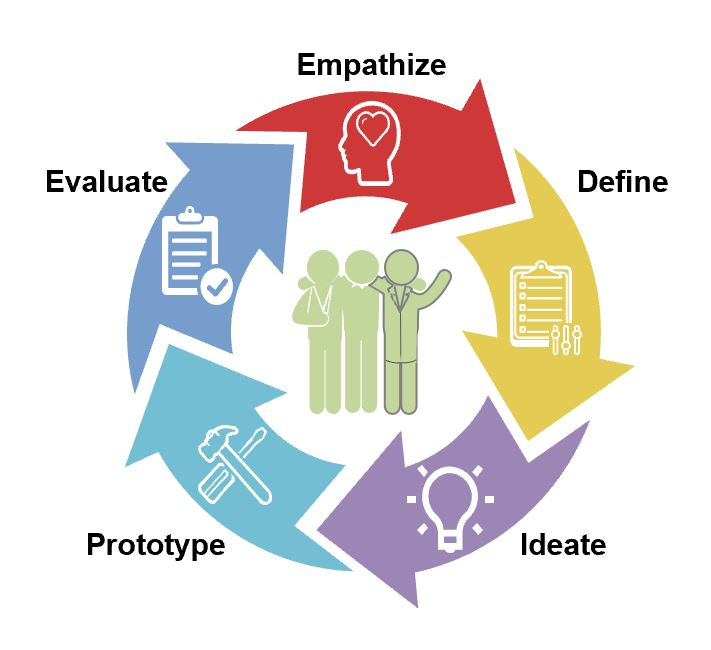
\includegraphics[width=0.75\columnwidth]{Images/Methods/ucd_flow.jpg}
	\caption{\textbf{The user-centered design method flow:} The method consists of five phases, empathizing, defining, ideating, protoyping and evaluating. The three users are involved in every step in order to iteratively improve the user experience.}
	\label{ucdflow}
\end{figure}
The user is present in every step in order to develop a final design matching the user’s needs \cite{buurmann1997}. \\
The mentioned target users form the user group were involved in every step of this project to get a broader spectrum of ideas, more accurate requirements and feedback on design aspects.

\begin{table}[bt]
\caption{Demographics of the spinal cord injured subjects}
\label{tab:specs_sci}
	\centering
	\begin{tabular}{lllll}
	    \hline
		& VariLeg enhanced & VariLeg enhanced & VariLeg II \\
		Attributes  & main pilot & Second pilot  & former pilot\\
		Reference & S1 & S2 & S3\\
		\hline
		Sex & male & male & male \\
		Age [y] & 32 & 29 & 59\\
		SCI since [y]  & 4 & 2 & 9 \\
		Lesion Height & Th 12& Th 5 & Th 12\\
		Classification* & ASIA A& ASIA A& ASIA A \\
		Experience level with\\ lower limb exoskeleton & novice & novice & experienced\\
		\hline
	\end{tabular}
\begin{tablenotes}
\centering \item *American Spinal Injury Association \cite{ASIA}
\end{tablenotes}
\end{table}

%\begin{enumerate}[i]
%\item VariLeg enhanced main pilot, advanced user, involved in every step
%\item VariLeg enhanced second pilot, novice user, involved during defining, ideating and evaluating
%\item Former VariLeg II pilot, experienced user, involved during empathizing and evaluating
%\end{enumerate}
%The VariLeg enhanced main pilot started using the exoskeleton during the project, the second pilot of the VariLeg enhanced exoskeleton has never walked with the exoskeleton until the end of this thesis research. The former VariLeg II pilot regulary used the exoskeleton for three consecutive years.

\subsubsection{Empathize}

To identify the problem and address the user's needs it is important to get to know the the user and state-of-the-art first, as established by Buurman (1997)\cite{buurmann1997}. For this purpose, S3 was recruited to assess the usability of the VariLeg II crutches. The assessment was done with all users S1, S2 and S3 using a custom questionnaire including a conversation.\\

\subsubsection{Define}
\label{sec:structure}

Out of the emphathizing phase requirements were deducted which were further amended during an interactive workshop with S1 and S2. 
Mechanical requirements were mostly given by the instruments needed in the crutch in order to properly control the exoskeleton. The load case requirement was defined by first measuring the forces applied the crutch by the pilot S1 during standing up, sitting down and walking on even ground with force sensors mounted on the crutches. Afterwards, the peak forces with a safety factor of two were used as load case requirement, see app.\ref{subsec:define} and fig.\ref{fig:forcesensordata}.  \\
\\
The enhancement opportunities determined were then collected in a criteria catalogue and split into "must have", "nice to have" and "optimization" criteria. The "must have" criteria are essential in order to use the crutch with the exoskeleton. "Nice to have" criteria are functions to improve the user experience and the performance, but are not crucial for the crutch to fulfill its basic function. "Optimization" criteria are features that can be measured on a scale rather than just fulfilled or not fulfilled, e.g. the weight of the system. For example together with S1 the location of the haptic feedback was tested and defined.\\

\subsubsection{Ideate}
During an interactive workshop the pilots S1 and S2 together with engineers iteratively realized prototypes using rapid protoyping methods, such as cardboard, stickers to add buttons to the prototype and modelling clay. \\
Further ideas were worked out during state-of-the-art research, brainstorming sessions and free hand sketching.\\

\subsubsection{Prototype}
The user-centered design method requires prototypes specifically for the user in order to evaluate the product and help to iteratively improve the product. For the ergonomic handle design, it was crucial to use fast prototyping methods, so that the pilots could give feedback regarding the designs. Models made of modelling clay and later 3D printed models were used in order to receive fast results and to achieve more iterations. The length adjustment mechanism was also iteratively designed with 3D printed parts in order to establish a working mechanism in a minimal amount of time. As for the haptic feedback the position of the foot pressure sensor was iteratively adapted resulting from an analysis of the collected data.\\

\subsubsection{Evaluate}
The evaluation was done using a combination of different methods. For of the first 3D printed handle prototype a cognitive walk-through with a consecutive interview was conducted with pilot S1. The cognitive walk-through was carried out in a lab environment with three CYBATHLON competition obstacles: sitting down and standing up, walking on a tilted path and stairs up and down. The user S1 pressed the buttons on the crutches while holding them, the resulting movements were displayed by an assistant. The results were structured using an AD-SWOT analysis \cite{wu2009ucd} in a 2x2 matrix, categorizing the factors into positive and negative points as well as internal and external factors. The properties of the mechanical system were considered internal factors, whilst external factors are given through the user, CYBATHLON rules etc.\\
\\
For the evaluation the custom questionnaires with different statements were used, which were rated by S1 on a seven-point Likert scale \cite{likert}. The statements always included a comment field for the user to note additional feedback. Each questionnaires was filled out by S1 between one to three times on different occasions in order to get a more representative result. The custom questionnaires were mainly used to identify problems, find opportunities to further improve the system and track the improvement of individual functions and subsystems.\\
\\
The SUS \cite{brooke1996sus} was used to quantitatively evaluate the performance of the whole system and the three main subsystems: ergonomic crutch design, length adjustment mechanism and haptic feedback. The SUS is a standardized questionnaire with ten statements, five positively and five negatively formulated, which are rated on a five-point Likert scale. The answers are rated and summed up to a score for the whole system.\\
\\
Such a combination of standardized scales and custom-made questionnaire leads to an overall impression of the crutch’s performance. All questionnaires with the answers summarized can be found in app. \ref{subsec:evaluate}.

\section{Results}
Within this work, three different crutch features were developed and evaluated: \textit{(i.)} A standard closed-cuff Flexyfoot crutch was instrumented to control the VariLeg enhanced exoskeleton. This crutch was iteratively adapted to fit pilot S1's needs and antropometric measures and is herein referred as "ergonomic  crutch design". After working on the general crutch design, the added features \textit{(ii.)} and \textit{(iii.)}, defined in methods (see \ref{threegoals}), were developed. The added feature \textit{(ii.)} was integrated on a separate Flexyfoot crutch, referred to as "length adjustment mechanism"-crutch. In the following sections the results and design for each single component is presented. 
\\

\begin{figure}[!t]
	\centering
	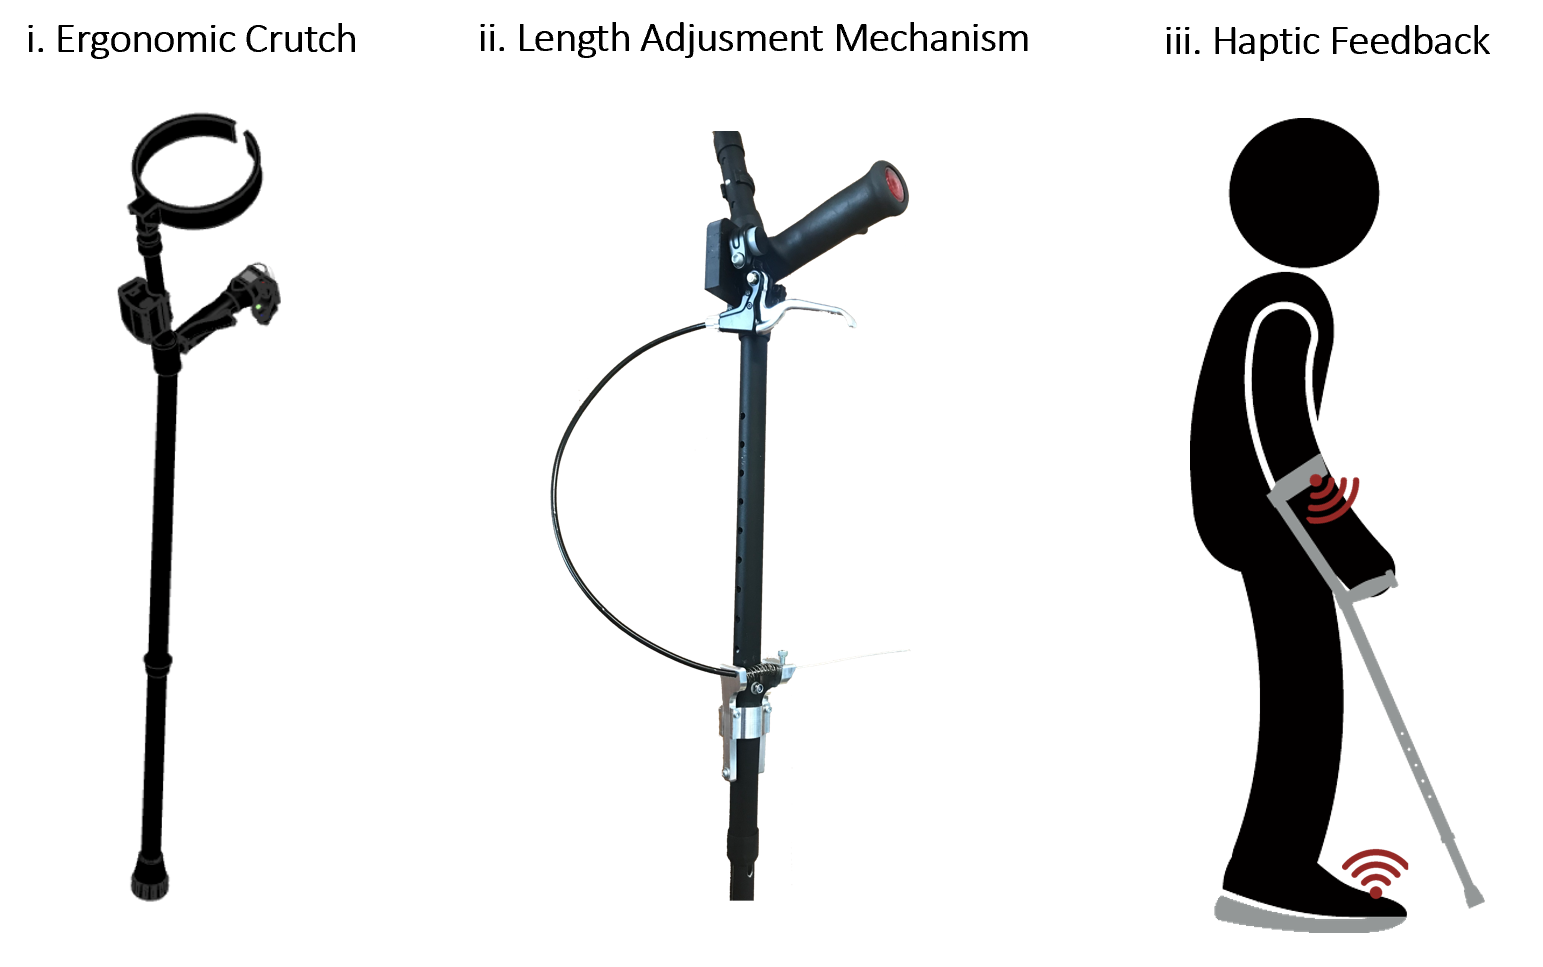
\includegraphics[width=0.75\columnwidth]{Images/Results/overview_goals.PNG}
	\caption{\textbf{Overview Goals:} The overall goal was to improve the usability of the VariLeg enhanced powered lower limb exoskeleton crutches. This consists of three objectives. (i) a to the pilot iteratively adapted control crutch design, refered to as ergonomic crutch. Secondly two additional features were conceived, (ii) a length adjustable crutch during use and (iii) a haptic feedback for the pilot to get more awareness of his movements.}
	\label{threegoals}
\end{figure}

\begin{enumerate}[\textit{i.}]
\item{\textit{Ergonomic Crutch Design}}
\end{enumerate}



The crutch is one of the main HRI of a lower limb exoskeleton; therefore, it is essential that the usability and ergonomics are enhanced. During user workshops the former crutches of the VariLeg II exoskeleton were found to still have weaknesses in terms of usability, that needed to be addressed. Especially, the placement and the size of the buttons seemed cumbersome to the pilot S3, since they lead to minor skin injuries on the fingers. Moreover, both crutches, left and right, were instrumented making it more difficult to use the exoskeleton with only one hand. This is necessary for example while climbing stairs, because the second hand is needed in order to hold the railing. Finally, the weight of the VariLeg II crutches, including force measuring sensors, summed up to 1.5 kg per crutch. The pilots S1 and S3 considered this as upper limit of what is bearable and, therefore, the upper weight limit of the new crutches was set to 1.5 kg.
The full list of resulting requirements out of the empathizing phase for the ergonomic crutch design can be found in app. \ref{subsec:EC requirements}. \\
\\
During user-workshops first the requirements were discussed and then designs were established. 
The users S1 and S2 had the possibility to integrate their design wishes into prototypes which were then modelled to achieve an individualized design, see fig. \ref{fig:handicraft}. As a result of the interviews with the pilots S1, S2 and S3, the design workshops and iterative adaptions a final design of the ergonomic crutch was developed, shown in fig. \ref{ergonomic_crutch}. The crutch base is a closed cuff Flexyfoot crutch. The crutch base was instrumented with the following additions in order to convert it into the control unit of the VariLeg enhanced exoskeleton: a cushioned closed cuff (1), a control handle unit (2), an electronic box (3) and a flexible foot (4). \\


\begin{figure}[!t]
	\centering
	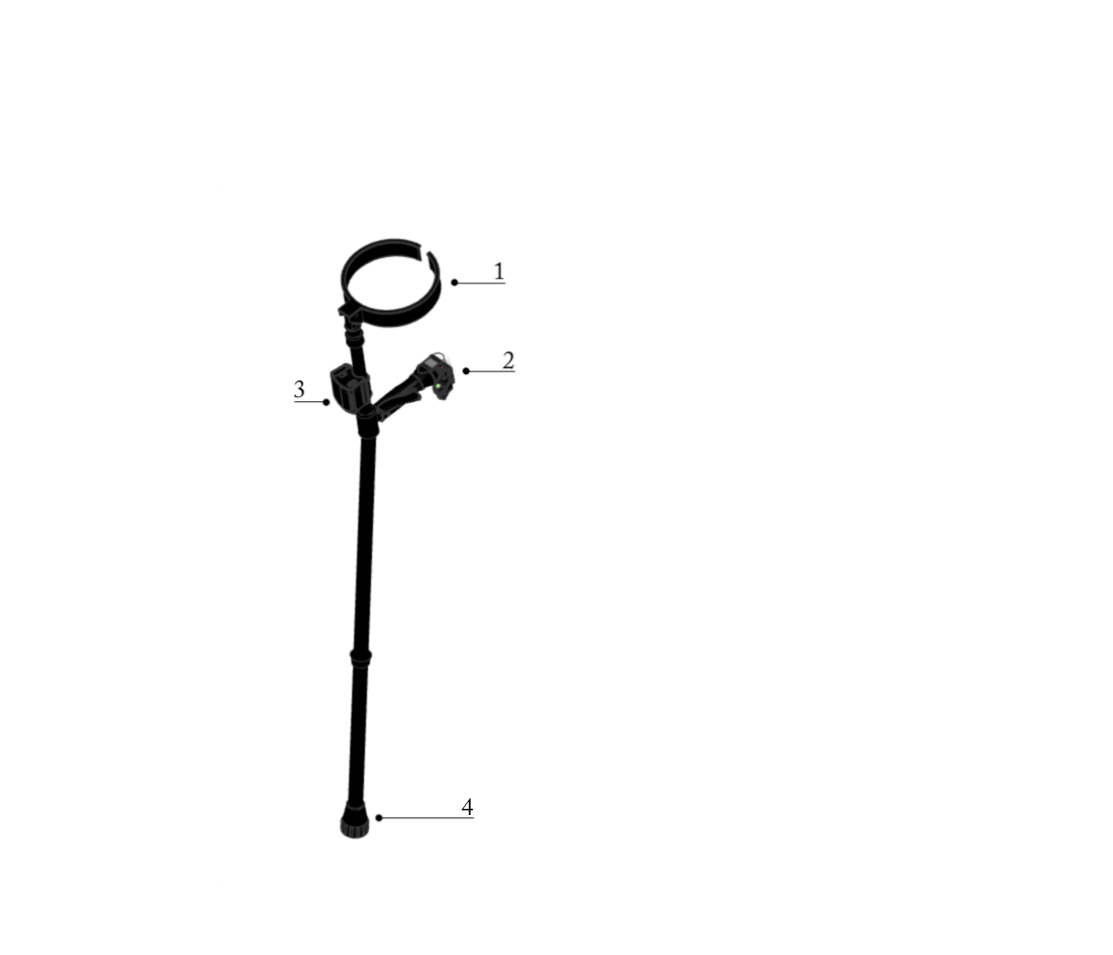
\includegraphics[width=1.5\columnwidth]{Images/Results/ergonomic_crutch.png}
	\caption{\textbf{Overview Ergonomic Crutch Design:} The crutch base was instrumented with a few additions in order to convert it into the control unit of the VariLeg enhanced exoskeleton: a cushioned closed cuff (1), a control handle unit (2), an electronic box (3) and a flexible foot (4).}
	\label{ergonomic_crutch}
\end{figure}

\begin{enumerate}[\textit{(1)}]
    \item{\textit{Closed Cuff}}
\end{enumerate}

\begin{figure}[!t]
	\centering
	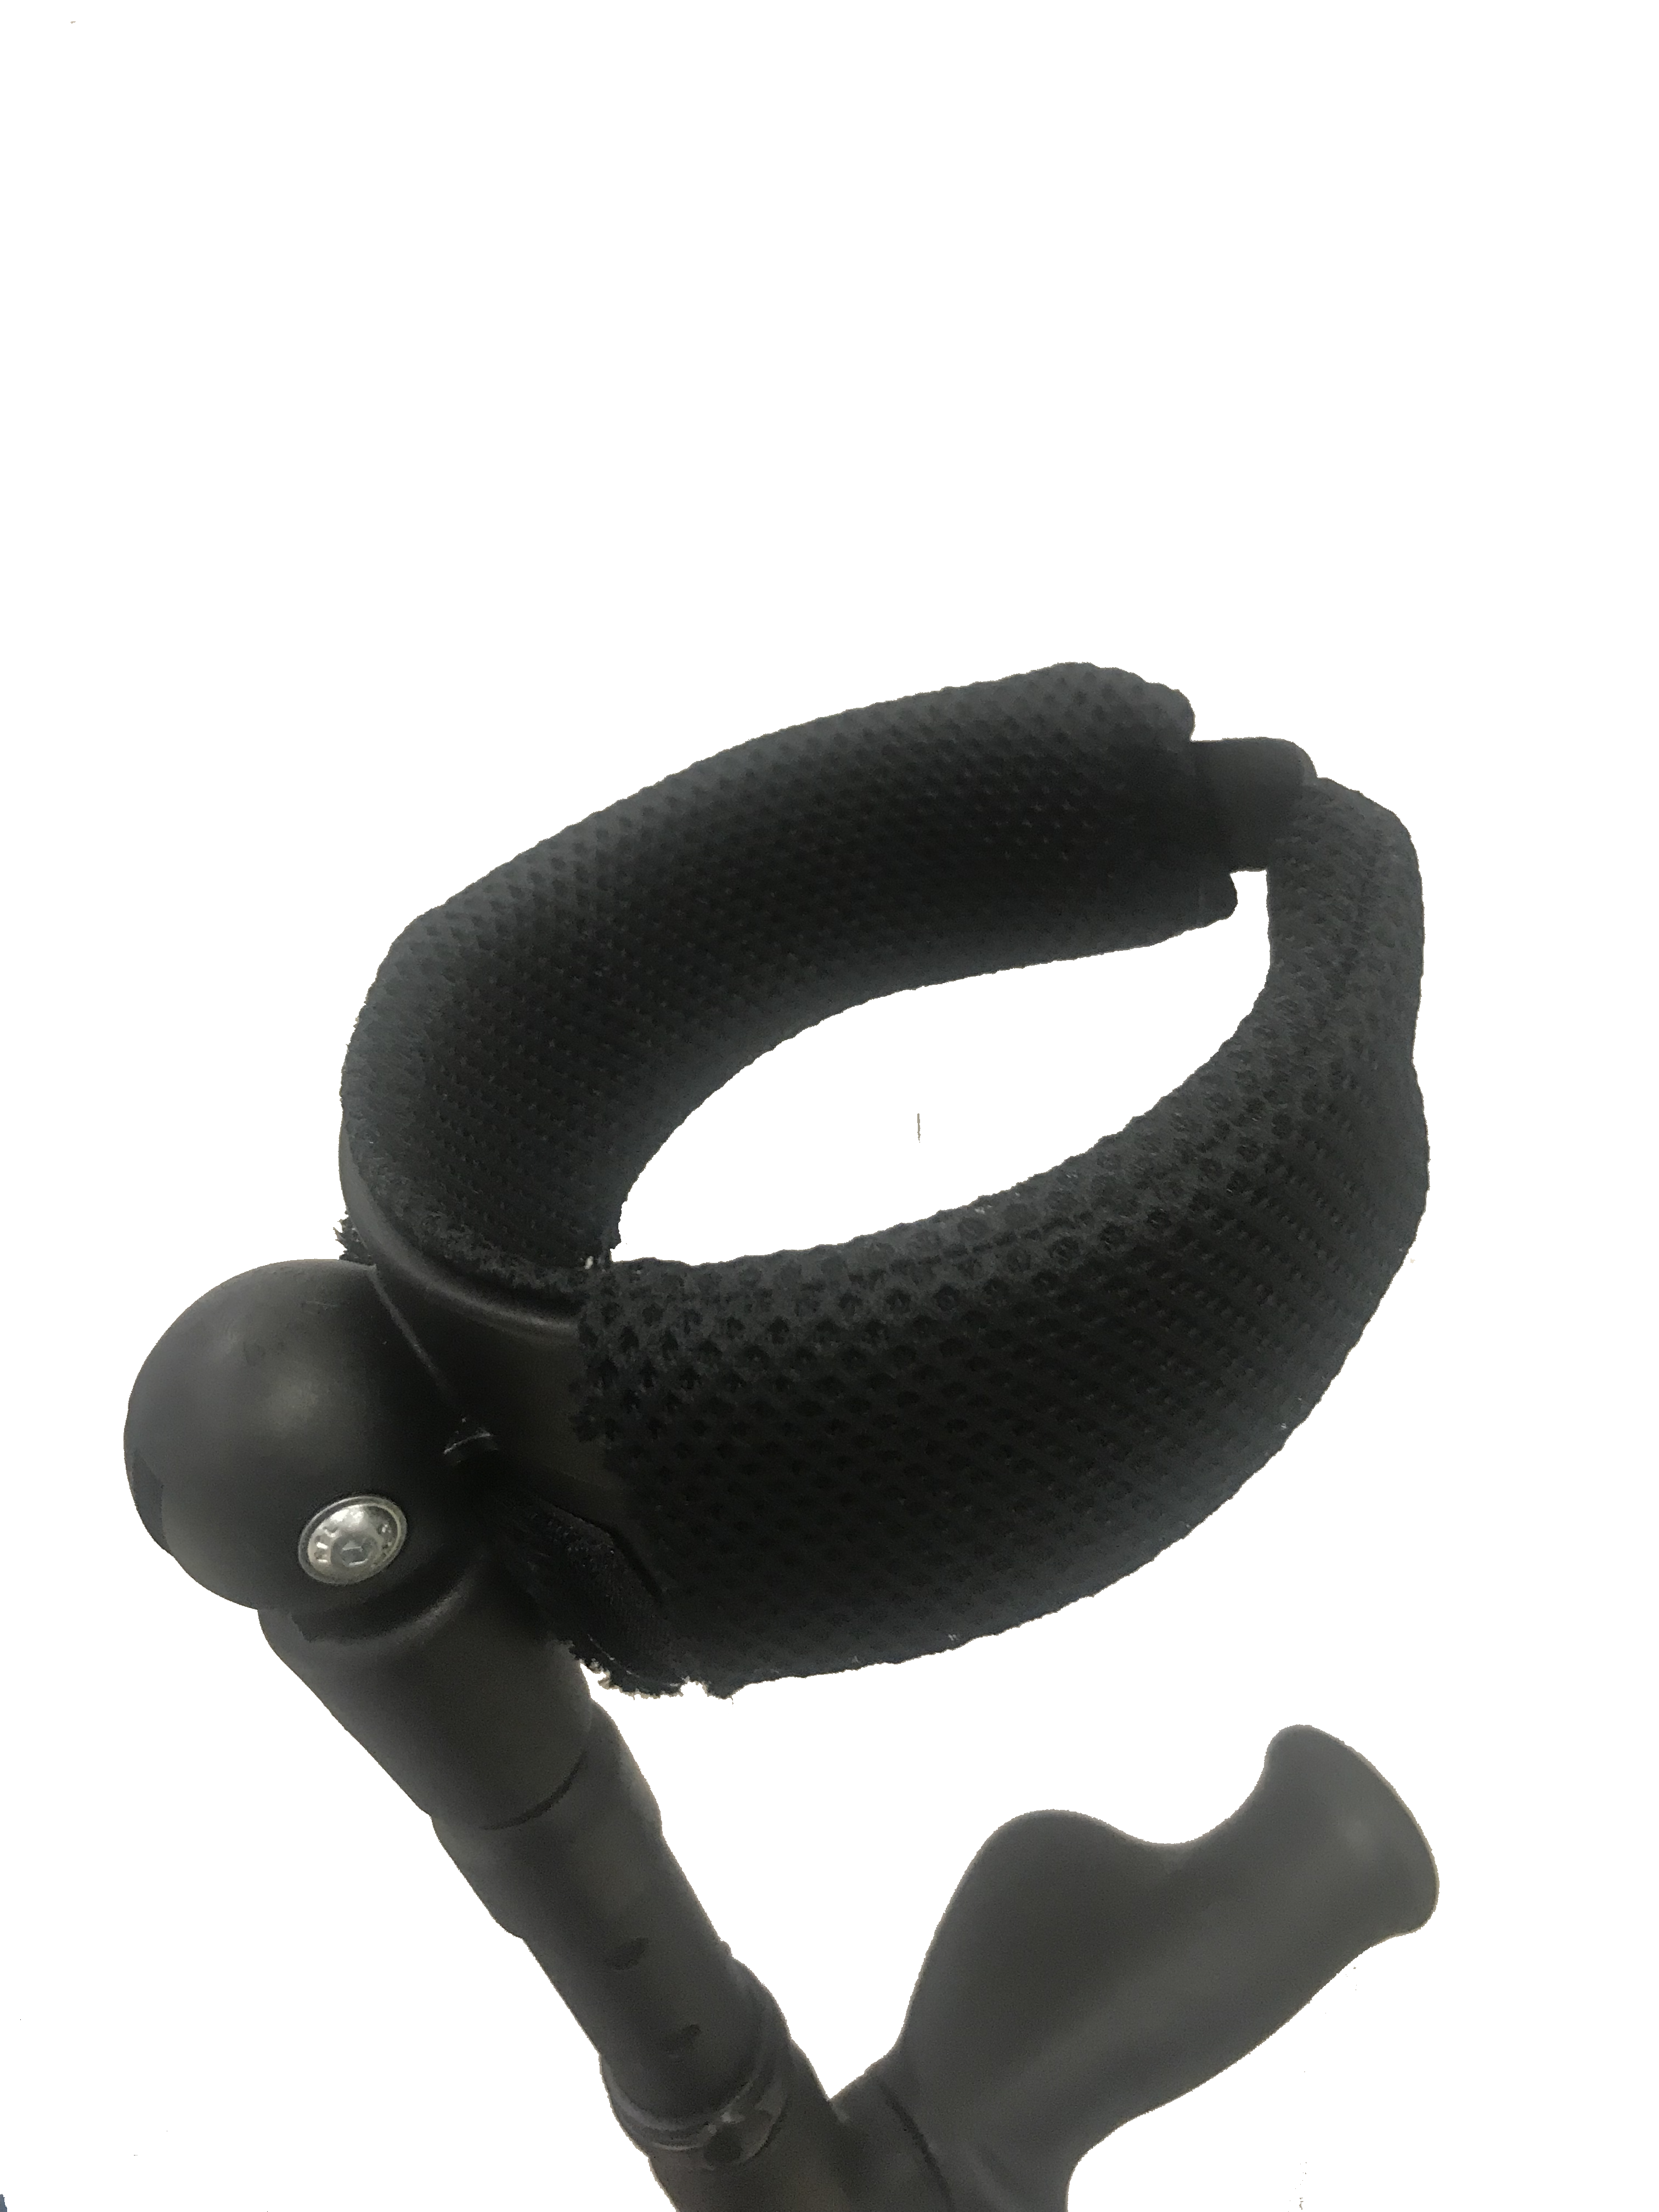
\includegraphics[width=0.75\columnwidth]{Images/Results/closed_cuff.png}
	\caption{\textbf{Closed Cuff including the One–Hand–Free Mechanism:} The cushioning includes a small ribbon, which prevents the pilot from losing the crutch while letting the handle go and moving his hand freely.}
	\label{closed cuff}
\end{figure}
In order to increase comfort, the closed cuff of the Flexyfoot crutch was cushioned with breathable textile. The cushioning includes a small ribbon, see fig. \ref{closed cuff}, which prevents the pilot from losing the crutch while letting the handle go and moving his hand freely.\\

\begin{enumerate}[\textit{(2)}]
    \item{\textit{Control Unit}}
\end{enumerate}

\begin{figure}[!t]
	\centering
	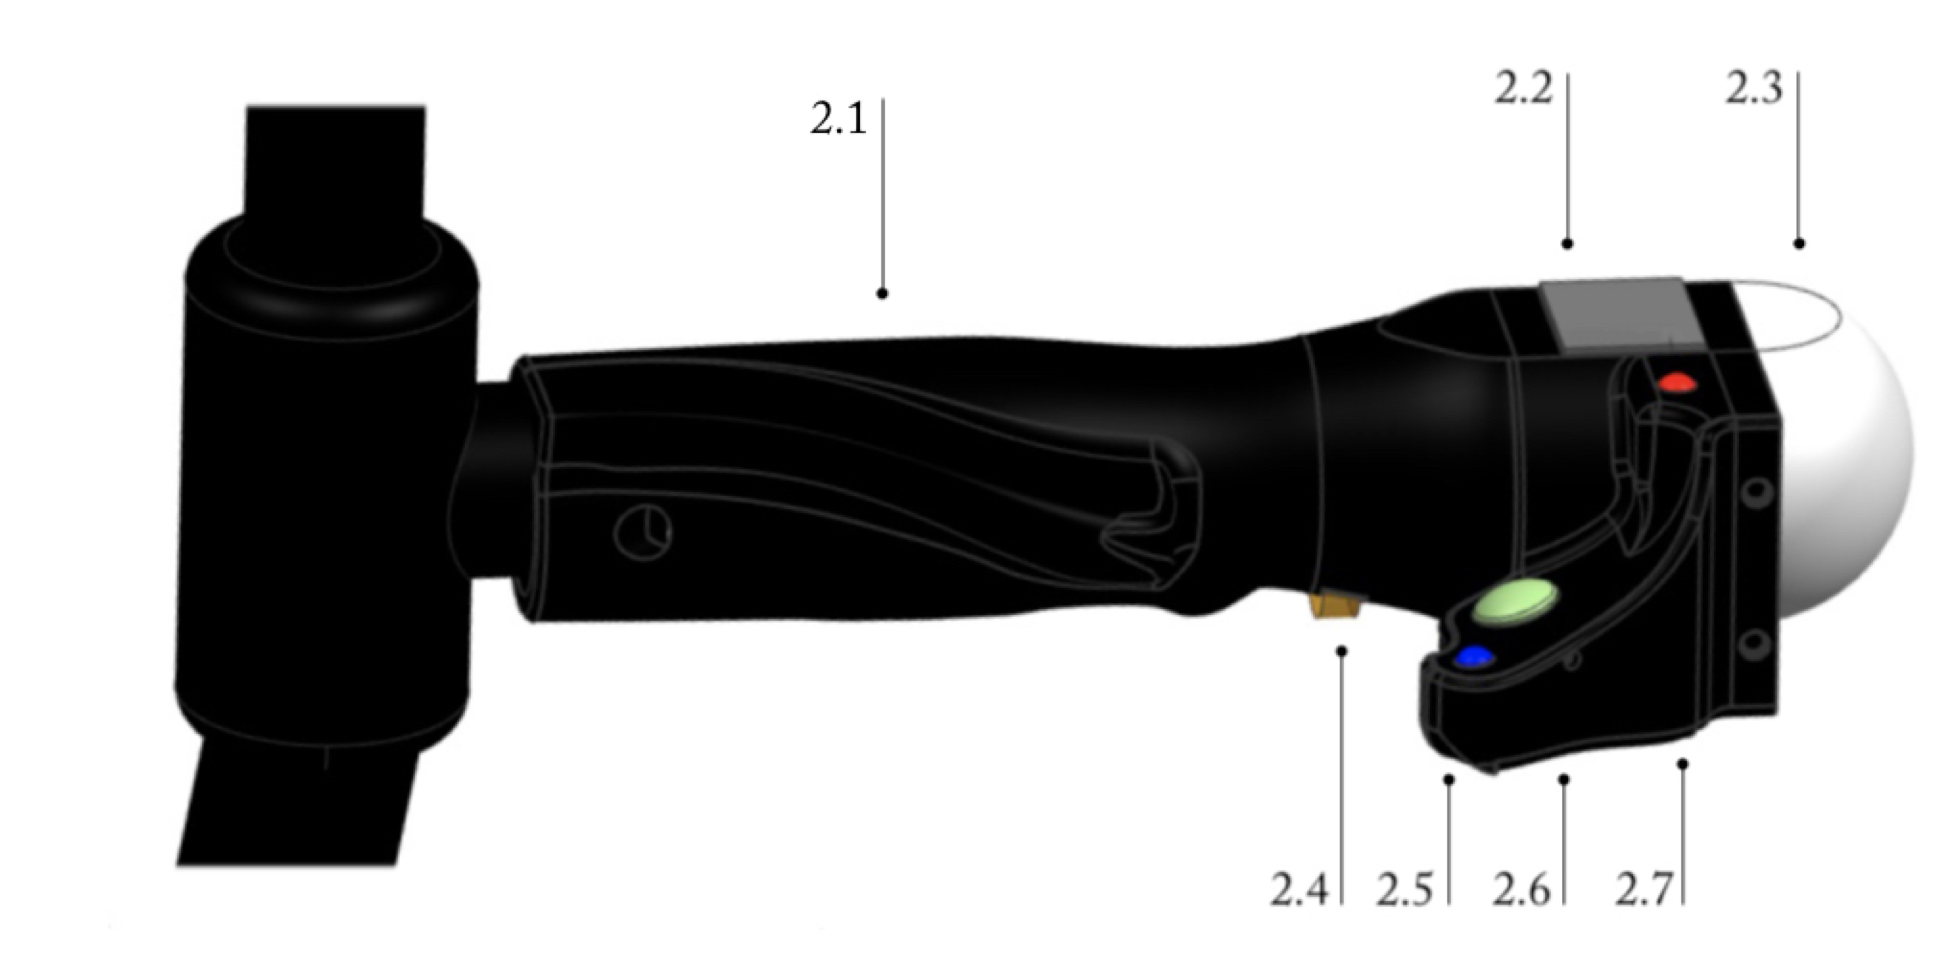
\includegraphics[width=1\columnwidth]{Images/Results/ergonomic_handle.png}
	\caption{\textbf{Ergonomic Handle and Control Unit Design:} It consists of the following elements: Ergonomic handle (2.1), two seven-segment displays showing the current mode and step length (2.2), an  RGB LED indicating the state of the crutch (2.3), a wheel to switch between the modes (2.4), a button to adjust the step length (2.5), a "Go" button to activate the next step (2.6) and a "Freeze" button to immediately stop the movement (2.7).}
	\label{ergonomic_handle}
\end{figure}
The Control Unit is located on the handle of the left crutch, see fig. \ref{ergonomic_handle}. After an evaluation with the pilot S1 the ergonomic handle of the VariLeg II crutches was adapted to achieve an individualized version (2.1), which is customized for the pilot S1. The two seven-segment displays show the current mode and step length (2.3). The modes go from 0 to 9 and the order of the modes was chosen to follow the CYBATHLON 2020 parkour as good as possible. A list of all modes can be found in app. \ref{subsec:list of modes}. The step length is displayed as horizontal lines: The screen shows the lowest horizontal line for step length one, the two bottom ones for step length two and all three lines for step size three, see fig. \ref{fig:steplength}. \\
\begin{figure}
    \centering
    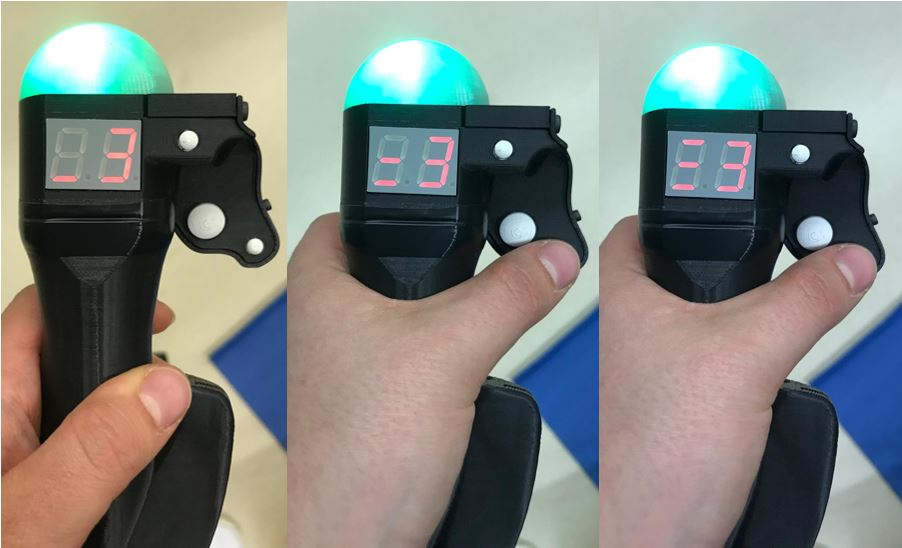
\includegraphics[width=1\columnwidth]{Images/Results/steplength.JPG}
    \caption{\textbf{Indication of step length:} The step length can be chosen from three different lengths, the chosen option is displayed with the amount of horizontal lines on the left display of the crutch.}
    \label{fig:steplength}
\end{figure}
Similarly, to the VariLeg II crutches a RGB LED is included in the front of the crutch (2.3). It indicates the state of the crutch by displaying different colors. Green indicates that the crutch is ready to receive an input, blue means the crutch is currently sending a signal to the main board computer and red is displayed if an error occurred or the pilot is in the Freeze-state.\\
The exoskeleton can be maneuvred with three buttons and one wheel. The wheel, which is located on the lower side of the handle, is used to switch modes (2.4). This placement allows the pilot to reach the wheel with his index finger. \\
The small blue button is used to adjust the step length while in the walking mode (2.5). The “Go" button is the most frequently used button, thus it is the largest button and placed at the most convenient position for the pilot S1 (2.6). The button triggers the next step when pressed. To reduce the source of human error, the button has to be pressed at least three seconds to trigger the first step after changing mode. The same is done to go back into parallel stand. The red “Freeze" button on top of the control unit triggers an immediate stop of the motion (2.7). The stopped motion can afterwards either be continued or reversed: For reversing the pilot needs to press the button shortly and long for continuation of the started movement. \\

\begin{enumerate}[\textit{(3)}]
    \item{\textit{Electronic Box}}
\end{enumerate}
In order to preprocess the inputs of the pilot, to communicate those to the exoskeleton and to display the feedback on the screen, the the ESP32 DevKit V4 microcontroller is included in the crutch, see app. \ref{subsec:HF ESP}. The microcontroller is connected to the main computer by an USB cable. The electronic box allows an easy storage of the microcontroller and a corresponding battery. After a usability evaluation with the pilot the box was redesigned to be more compact and located between the closed cuff and the handle in order to avoid collision with the thigh module of the exoskeleton.\\

\begin{enumerate}[\textit{(4)}]
    \item{\textit{Crutch Foot}}
\end{enumerate}
The crutch foot needs to provide the pilot enough grip during the CYBATHLON. On the one hand side, the Flexyfoot was used most of the time, which can adapt to the ground and thereby, compensate some unevenness on the ground. The Flexyfoot was already implemented in the VariLeg II crutch. Alternatively, a three feet tip was tested, which was expected to give more stability. However, the three feet tip did not have enough grip leading to insecurity. 

\begin{figure}
    \centering
    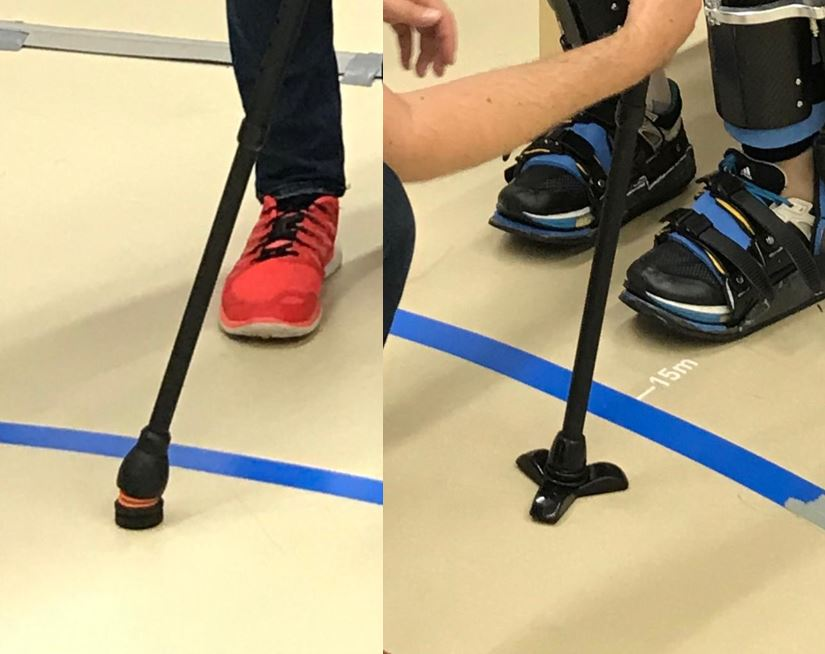
\includegraphics[width=1\columnwidth]{Images/Results/feet.JPG}
    \caption{\textbf{Flexyfoot and Three Feet Tip:} Two different crutch feet were tried out to achieve enough grip and flexibilty.}
    \label{fig:LAM}
\end{figure} \\


%\subsubsection{Requirements of the ergonomic crutch design}
%Most of the requirements which resulted from the emphasizing and the defining phase are fulfilled with the final design. Out of the Must have Criteria’s only one was not met: The Control Unit (2) did not withstand all the forces applied. The resulting clearance needed to be glued together. Three of the Optimization Criteria’s were completely achieved. The others include for example the facility of maintaining of the crutch and the amount of modes. Five out of nine Nice to have Criteria’s five are fulfilled. A wireless communication connection to the main computer was not yet implemented and the pilot cannot trigger the next movement before during the step.\\

\begin{enumerate}[\textit{(5)}]
    \item{\textit{Evaluation of Ergonomic Crutch}}
\end{enumerate}
The conducted SUS with the ergonomic crutch design showed an average score of 90 for S1, 75 for S2 and 87.5 for S3. The evaluation with the custom questionnaire showed very good results in general. The first two evaluation rounds clearly implied the positioning of the electronic box being troubling. After implementing the new electronic box design, all the answers in the custom questionnaire were rated positively on the Likert Scale by the pilot S1.\\

\begin{enumerate}[\textit{ii.}]
\item{\textit{Length Adjustment Mechanism}}
\end{enumerate}
Shoulders are the most important joints for a person with paraplegia, because the arms compensate for the lack of lower limb functionalities. It is therefore important to take care of an ergonomic shoulder pose. During standing up in the exoskeleton the shoulders are positioned in an unergonomic pose. Therefore, a new concept of length adjustable crutches was developed allowing the length to be changed dynamically during use and thus aiming to counteract this position. Additionally, length adjustable crutches could help the pilot to shift his weight while walking on a tilted path, which is perceived very cumbersome by pilot S1.
The problem was substantiated by defining requirements with S1. The system must be as light weight as possible, a maximum of 0.5 kg was decided to not exceed the overall requirement of 1.5 kg. The mechanism should provide at least 15 cm adaptability in order to compensate for the tilted path and reduce the amount of abduction in the shoulders while sitting and holding the crutches.
On the market there exist length adjustment mechanisms like a gas spring of an office chair or remote telescope seat posts for mountain bikes. However, none of the commercial solutions fulfilled the determined requirements sufficiently. A new concept inspired by a bicycle break mechanism was therefore implemented. A detailed list of the requirements and the comparison of the solutions with the requirements can be found in app. \ref{subsec:LAM}.


\begin{enumerate}[\textit{1)}]
    \item{\textit{Prototype}}
\end{enumerate}
The design of the length adjustment mechanism can be seen in fig.\ref{fig:LAM}. It consists of a clamp mechanism (3.3) which holds the pipes in place relative to each other. The clamp can be opened with the handle (3.1) and a spring (3.2) inside of the upper pipes pushes the pipes apart from each other to elongate the crutch. In order to shorten the crutch, the user has to press against the spring. While shortening and extending the crutch a pin through a slot in the lower pipe indicates the end positions and simplifies the locking the crutch.
\begin{figure}
    \centering
    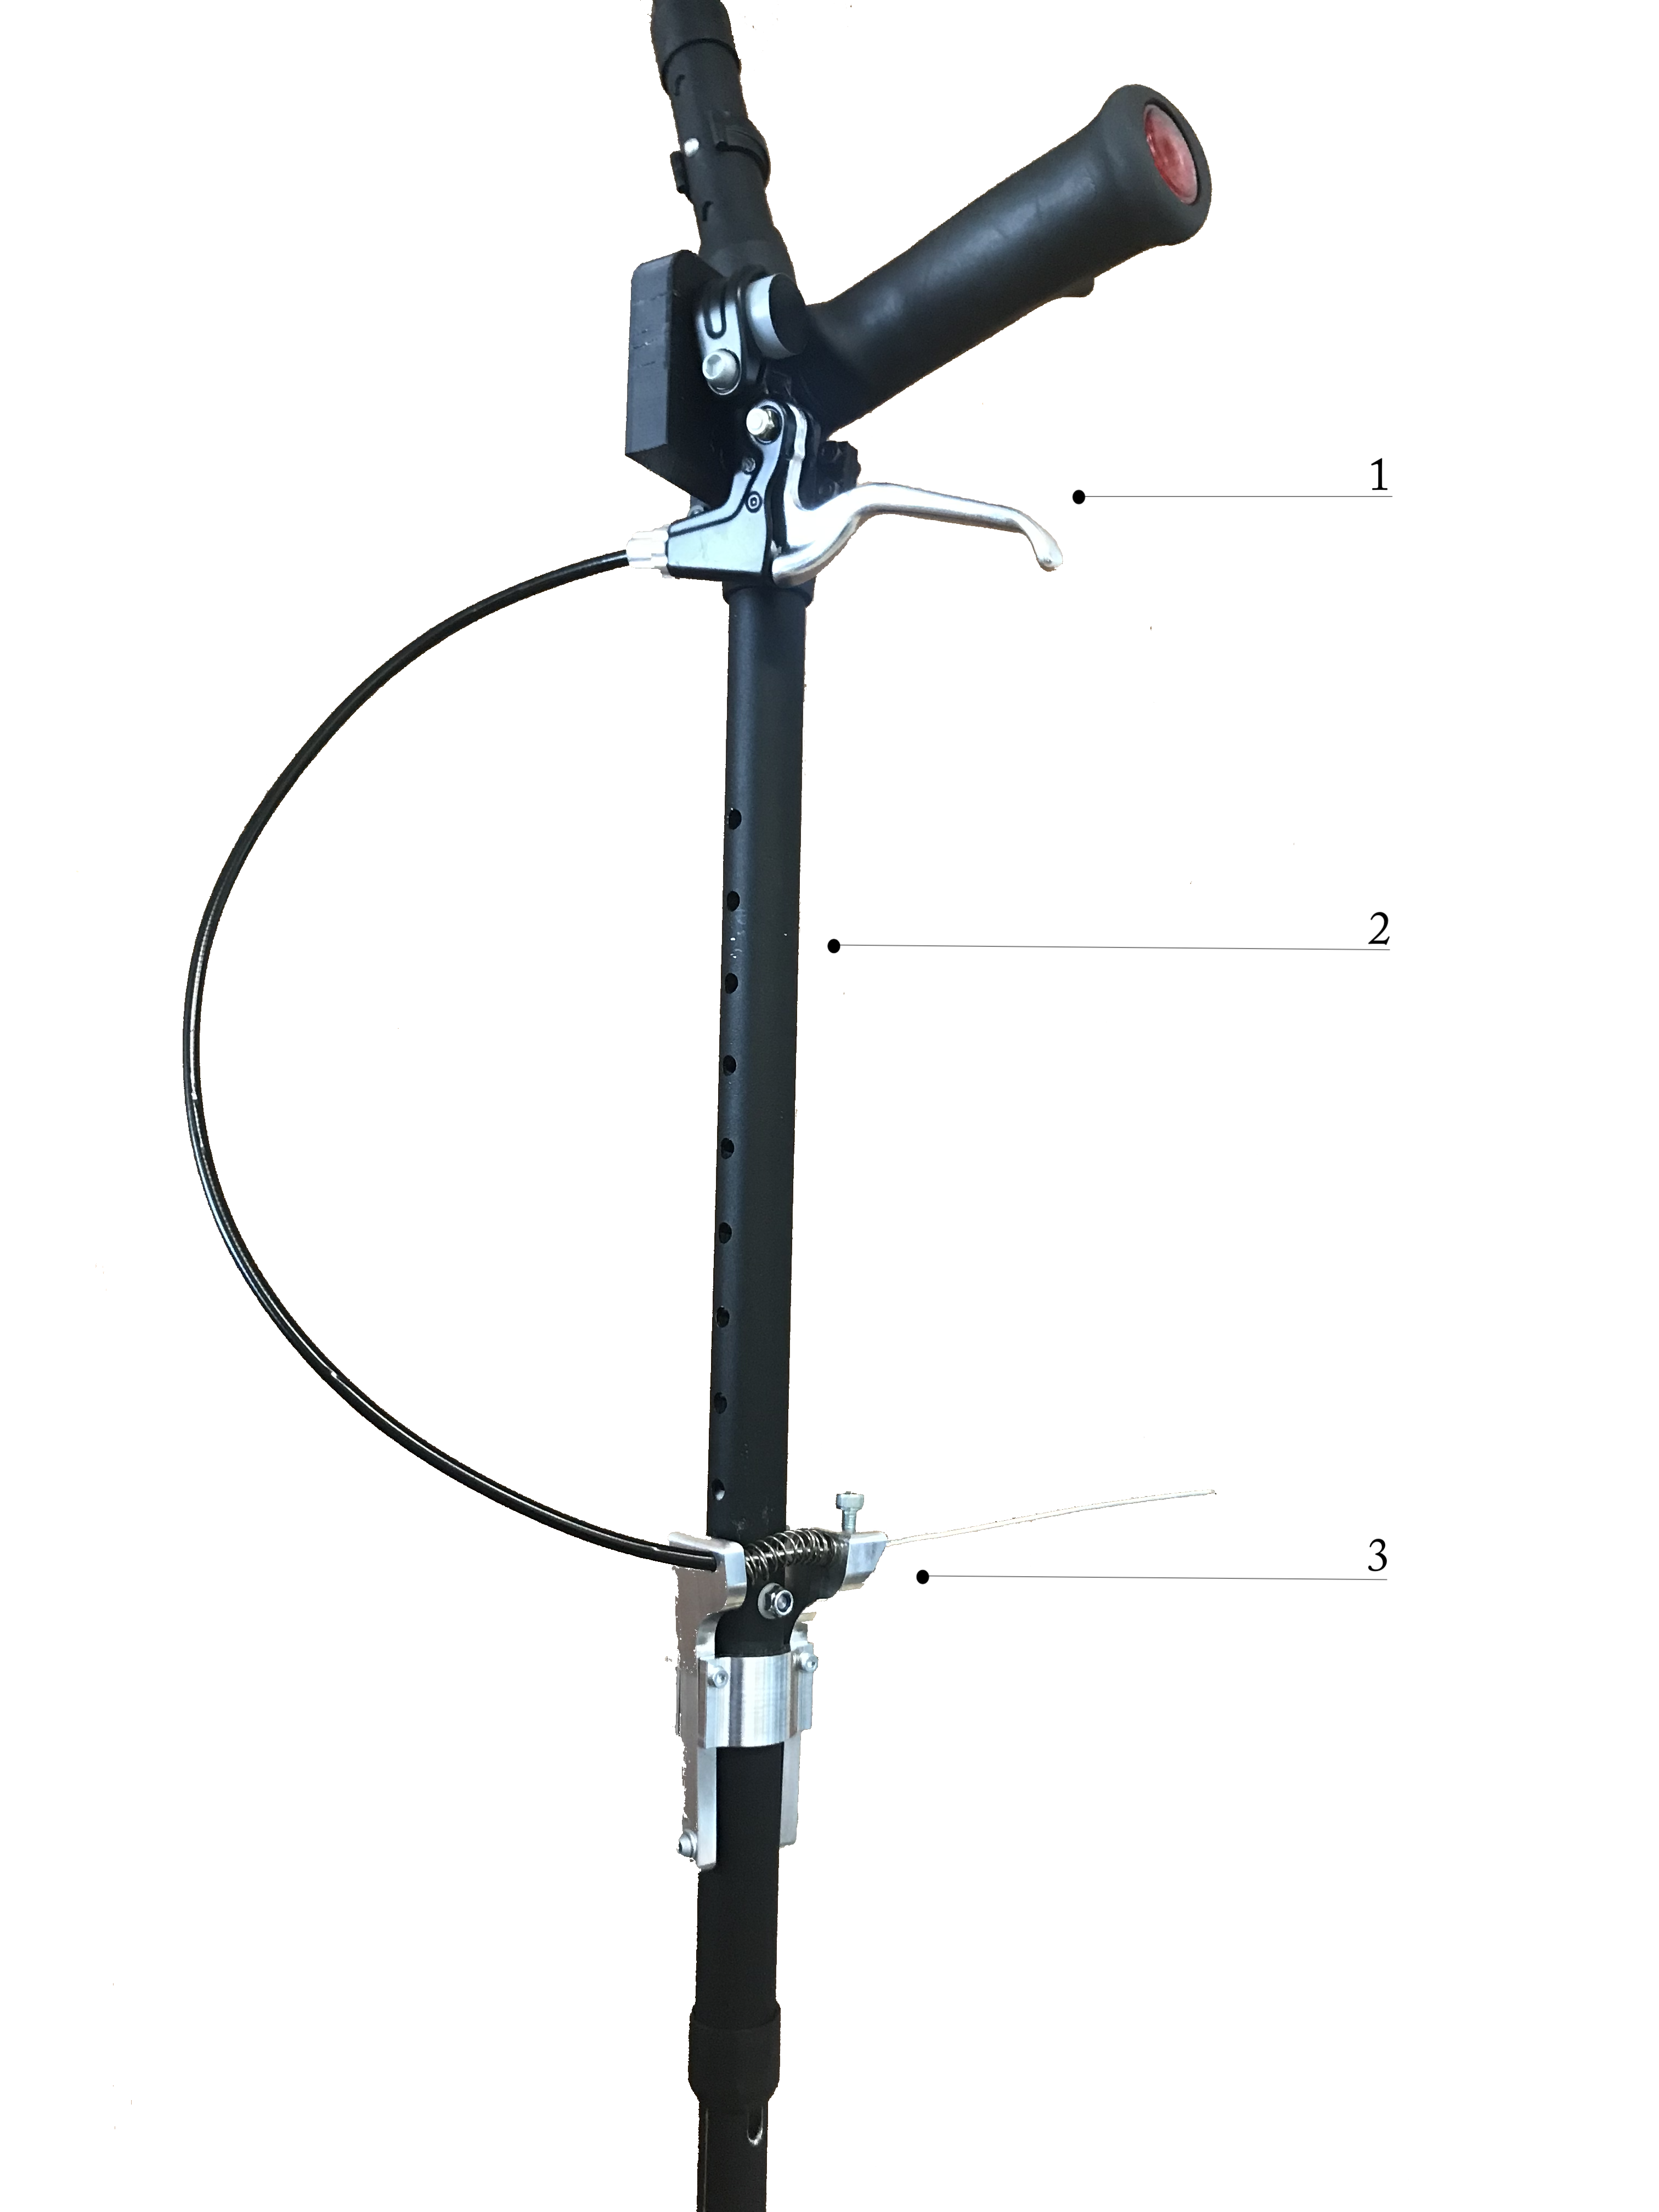
\includegraphics[width=1\columnwidth]{Images/Results/LAM.png}
    \caption{\textbf{Dynamic Length Adjustment Mechanism} includes a handle (1) to open the clamp (2) with pins locking the crutch pipes. The upper pipe (3) holds a spring to push the pipes apart to extend the crutch.}
    \label{fig:LAM}
\end{figure}
When the crutch is elongated the spring is preloaded with around 25N, which is necessary to overcome friction between the pipes and move relative to each other. The crutch can be shortened 15cm from the natural walking length. If shortened the spring is loaded with 150N or 100N, depending on the spring used. This force enables the user to lengthen the crutch extremely fast, which is needed so the pilot in the exoskeleton does not lose balance while extending the crutch. The compression spring was dimensioned to meet these requirements, the details can be found in app. \ref{subsec:LAM}, as well as additional figures of the bottom crutch pipe fig.\ref{fig:pin_LAM} and the clamp mechanism fig. \ref{fig:CAD_LAM}. \\

\begin{enumerate}[\textit{2)}]
    \item{\textit{Evaluation of Length Adjustment Mechanism}}
\end{enumerate}
In the custom questionnaire the length adjustment mechanism was rated easy to use and intuitive. It was also evaluated that it is helpful for standing up and walking on a tilted path, but not needed for sitting down with the exoskeleton. The answers suggested that the initially tried force of 150N is too strong, it is cumbersome to collapse the crutches. The main problem arising after the first tests was the reliability of the mechanism, since the clamp did not always snap back in.\\
On the SUS scale the system scored 80 for S1 and 67.5 for S2. \\

\begin{enumerate}[\textit{iii.}]
\item{\textit{Haptic Feedback}}
\end{enumerate}

During walking in the exoskeleton the pilot cannot feel, when his feet are touching the ground and at what moment the shifting of his weight is ideal. Visual feedback is necessary resulting in a bent position of the upper body, as can be seen in fig. \ref{motivation_haptic_feedback}. In order to achieve a more ergonomic positioning of the upper body, additional feedback should be included.
\begin{figure}[!t]
	\centering
	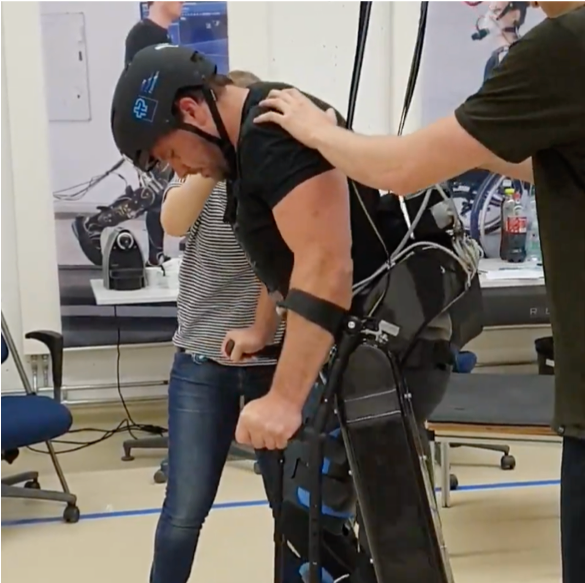
\includegraphics[width=1\columnwidth]{Images/Results/motivation_haptic_feedback.png}
	\caption{\textbf{Motivation for Haptic Feedback:} During walking in the lower limb exoskeleton the pilot has a bent positioning of the upper body in order to see the movement and to know when the weight can be shifted.}
	\label{motivation_haptic_feedback}
\end{figure}
Through a custom questionnaire and user interviews with S1, S2 and S3 during the emphathizing and defining phase haptic feedback was considered to be the most promising solution. Implementing such a haptic feedback has already proven to help spinal cord injury patients perceive the position of a virtual leg during studies \cite{solaimanshokur}. Additionally, an evaluation of a haptic feedback system for a lower limb exoskeleton showed that the integration of the feedback into the crutch module could be beneficial \cite{GerhardKuert}.
%Thus, the main requirement of this additional feature is that at the moment of ground contact a haptic feedback in the crutch should be given, in order to allow the pilot to stand more upright and know when the full weight can be shifted. \\ 
\\
The defined setup to realise a haptic feedback consists of the foot module and the feedback module, see fig. \ref{Haptic_Feedback_Overview}. The IEE foot pressure sensor combined with a self-designed printed circuit board (PCB) and a microcontroller were used to read out the pressure applied on the foot. Digital signal are then published to the crutch's microcontroller which activates a flat coin vibration motor.\\
\begin{figure}[!t]
	\centering
	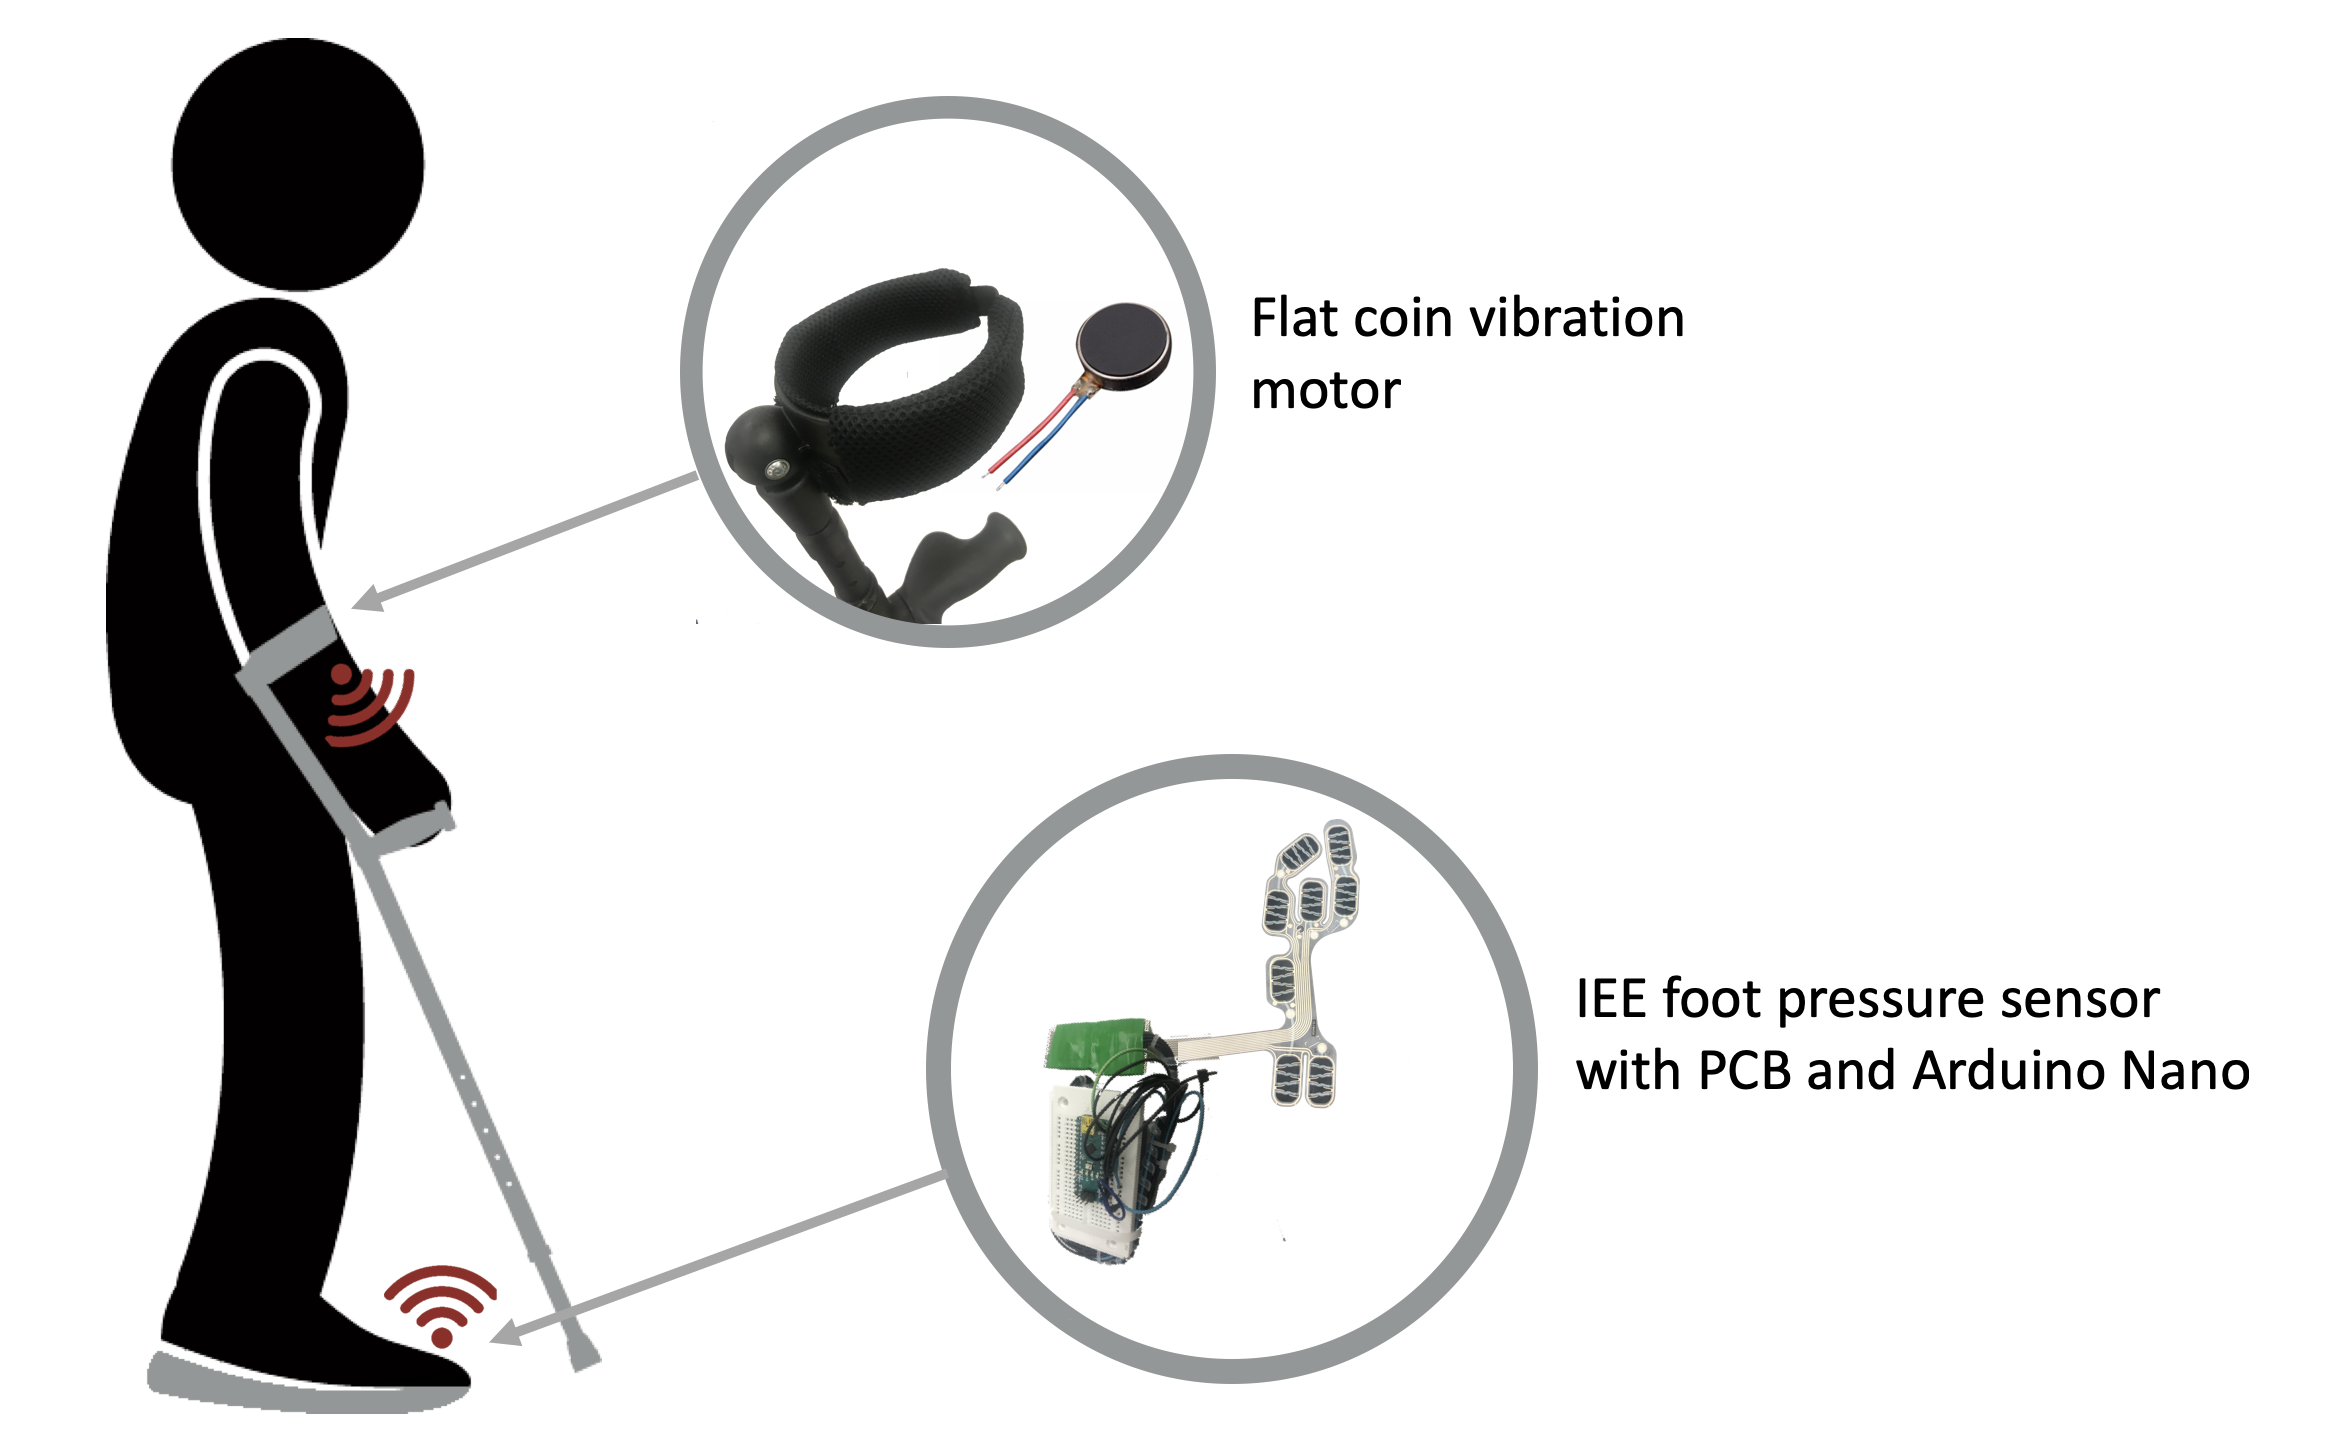
\includegraphics[width=1\columnwidth]{Images/Results/Haptic_Feedback_Overview}
	\caption{\textbf{Overview to the Setup of Haptic Feedback:} The haptic feedback consists of two modules: The foot module containing a IEE foot pressure sensor combined with a self-designed PCB and a microcontroller. The vibration module is a flat coin vibration motor which is integrated in the crutch's electronics. The two communicate over a serial connection through the main computer. }
	\label{Haptic_Feedback_Overview}
\end{figure}
This setup resulted in further requirements: A reliable recognition of the gait cycle through an implemented foot sensor in the foot module sets the foundation for the haptic feedback signal. To give back the feedback signal a vibration motor with the right strength is needed, such that the pilot is not distracted from walking, but still recognizes the signal substantially. To connect the two modules, a robust transmission is needed. The more detailed list of requirements can be found in app. \ref{subsec:HF requirements}. \\
\\
\begin{enumerate}[\textit{1)}]
    \item{\textit{Vibration Module}}
\end{enumerate}
In collaboration with S1 the requirements for the vibratory feedback were elaborated: It should be integrated on the inside of the closed cuff of the crutch so that the pilot S1, see app. \todo{appendix}. Additionally, only one input should be given at the moment of heel strike. The full interview can be found in app. \todo{appendix}.

\begin{enumerate}[\textit{2)}]
    \item{\textit{Foot Sensor Module}}
\end{enumerate}


The IEE foot pressure sensors work with eight force sensing resistors (FSR) \cite{Footsensor}, which use variable resistance to measure pressure applied to the sensor cell, see app. \ref{subsec:HF Insole} . Meaning that the pressure can be measured electronically by implementing a voltage divider for each cell. The corresponding schematics can be found in app. \ref{fig:schematics}. In order to implement the foot sensors compactly on both sides, a PCB for the ESP 32 Dev Kit V4 was developed, see \ref{subsec: HF PCB}. \\
The microcontroller in the foot module measures the voltage, which can then be correlated to the pressure applied, see app. \ref{subsec:HF Insole}. To avoid a trigger of a false haptic feedback by only a few outliners, a combination of a moving average filter and a transition recognition was used.\\
\\
To better understand the sensor an additional calibration of the foot pressure sensor was conducted where each cell was tested independently with a load of 5 kg found in \ref{tab: calibration} and the forces from 1 kg to 5 kg were applied to one cell to analyze the sensitivity of the sensor cell seen in table \ref{tab:footsensor}.\\ 
\begin{table}[!t]
	\renewcommand{\arraystretch}{1.3}
% if using array.sty, it might be a good idea to tweak the value of \extrarowheight as needed to properly center the text within the cells
	\caption{Data of the calibration of the IEE foot sensor}
	\label{tab:footsensor}
	\centering
% Some packages, such as MDW tools, offer better commands for making tables
% than the plain LaTeX2e tabular which is used here.
		\begin{tabular}{l|ccc}
			\hline
			Load [kg] & Mean [V] & Standard Deviation [V] & CV Value [ ]\\ \hline 
			1  & 0.1375 & 0.1024 & 0.7447 \\
			2  & 0.2371 & 0.0884 & 0.3727 \\
		    3 & 0.3286 & 0.0377 &  0.1146 \\
			4 & 0.3583 & 0.0346 & 0.0965 \\
			5 & 0.4211 & 0.0437 & 0.1038 \\
			\hline
		\end{tabular}
\end{table}

\begin{enumerate}[\textit{3)}]
    \item{\textit{Placement and Gait Cycle recognition}}
\end{enumerate}
To implement the foot sensor into the exoskeleton the placement plays an important role. The foot attachment of the VariLeg enhanced exoskeleton can be seen in fig. \ref{foot_attachment_1}. Since the exoskeleton is still in developing phase the foot attachment was changed during the course of this thesis. The new foot attachment, the outer sole, is displayed in fig. \ref{foot_attachment_2}. The following analysis refers to the first used foot attachment of the exoskeleton. \\
When used by a neurologically intact pilot the gait cycle of a step is displayed by the foot pressure sensor as can be seen in fig. \ref{Gait_Cycle_1}. To obtain these measurements the foot sensor was placed between the pilot's foot and the shoe of the exoskeleton. \\
\\
\begin{figure}[!t]
	\centering
	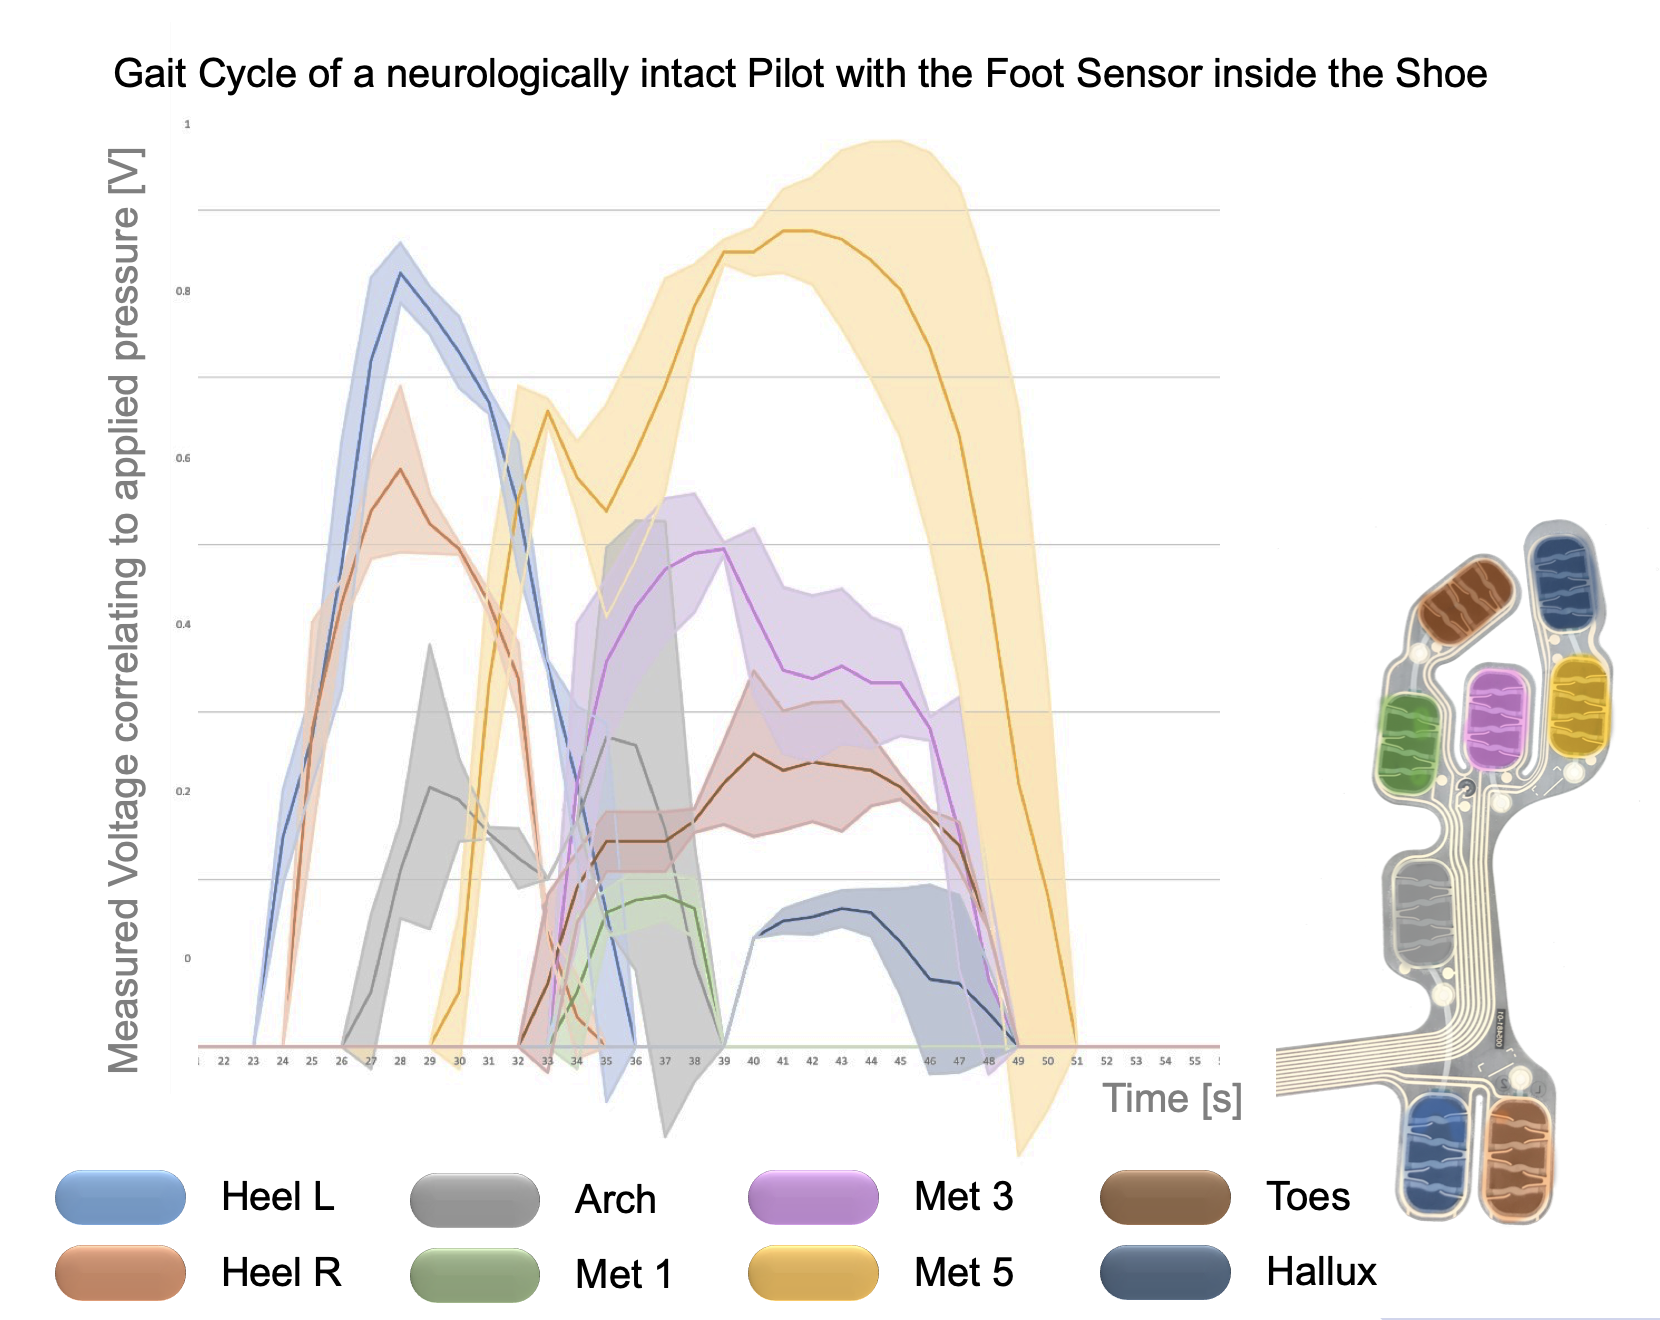
\includegraphics[width=1\columnwidth]{Images/Results/Gait_Cycle_1}
	\caption{\textbf{Measured Voltage during walking with a neurologically intaxt pilot}: This plot displays the mean and the standard deviation of measurements with a neurologically intact pilot with the pressure sensor located on the inside the shoe for each sensor cell.}
	\label{Gait_Cycle_1}
\end{figure}
Two positions of the foot sensor were tested with the pilot S1, inside the shoe, meaning between the exoskeleton's shoe and the pilot's foot, and outside the shoe, situated below the outer sole, see fig. \ref{Gait_Cycle_2} and \ref{Gait_Cycle_3}.
\begin{figure}[!t]
	\centering
	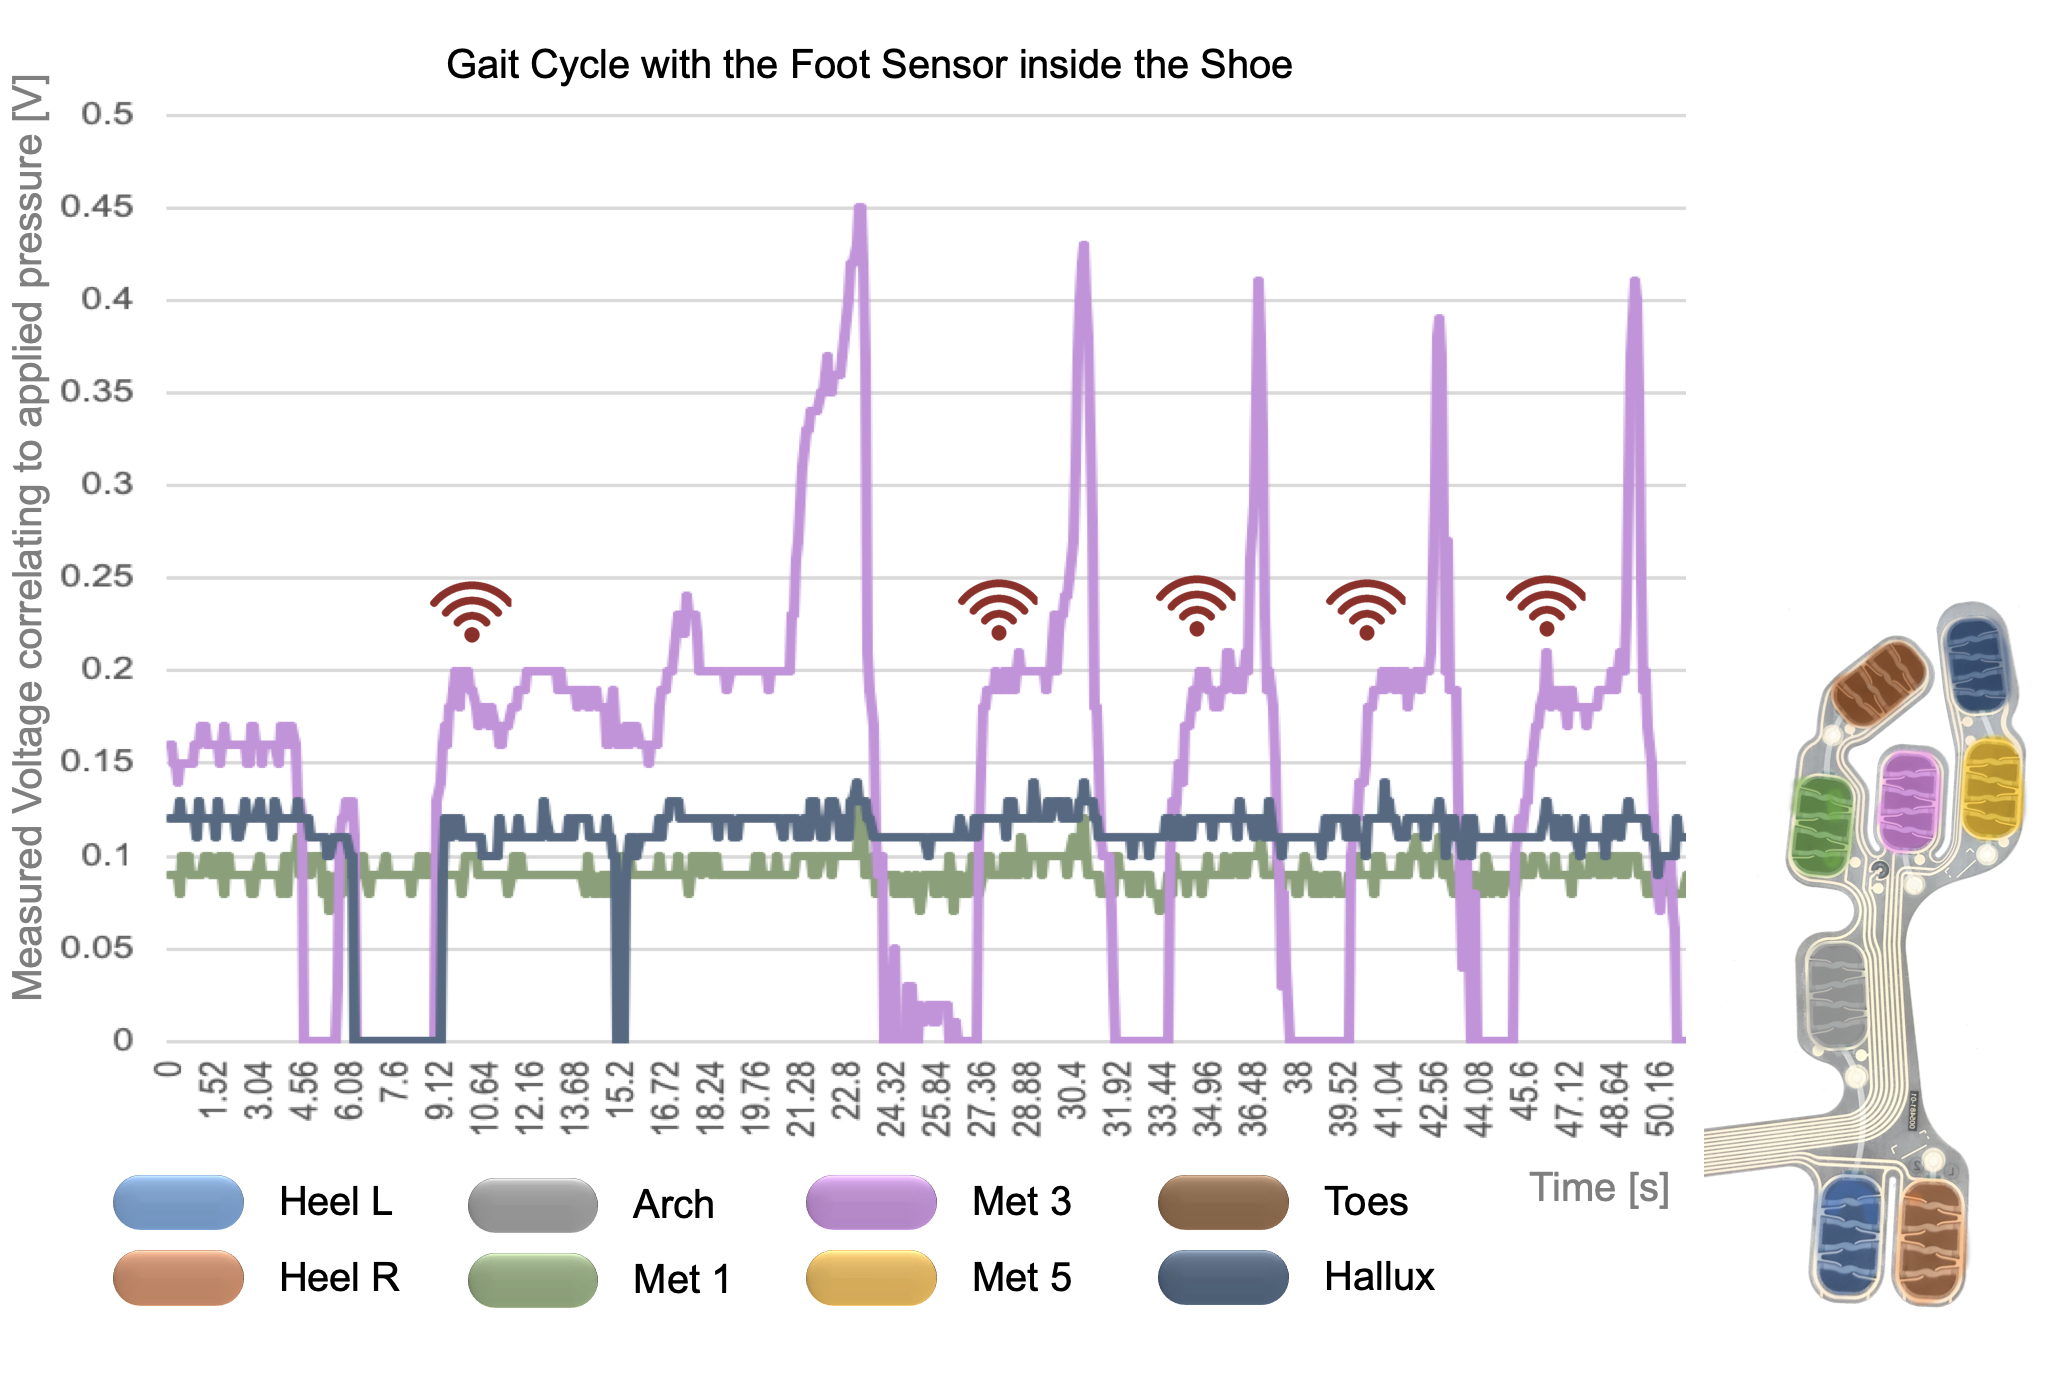
\includegraphics[width=1\columnwidth]{Images/Results/Gait_Cycle_2}
	\caption{\textbf{Measured values for a paraplegic pilot during walking in the exoskeleton with the pressure sensor between inner and outer sole of the shoe.}}
	\label{Gait_Cycle_2}
\end{figure}
\begin{figure}[!t]
	\centering
	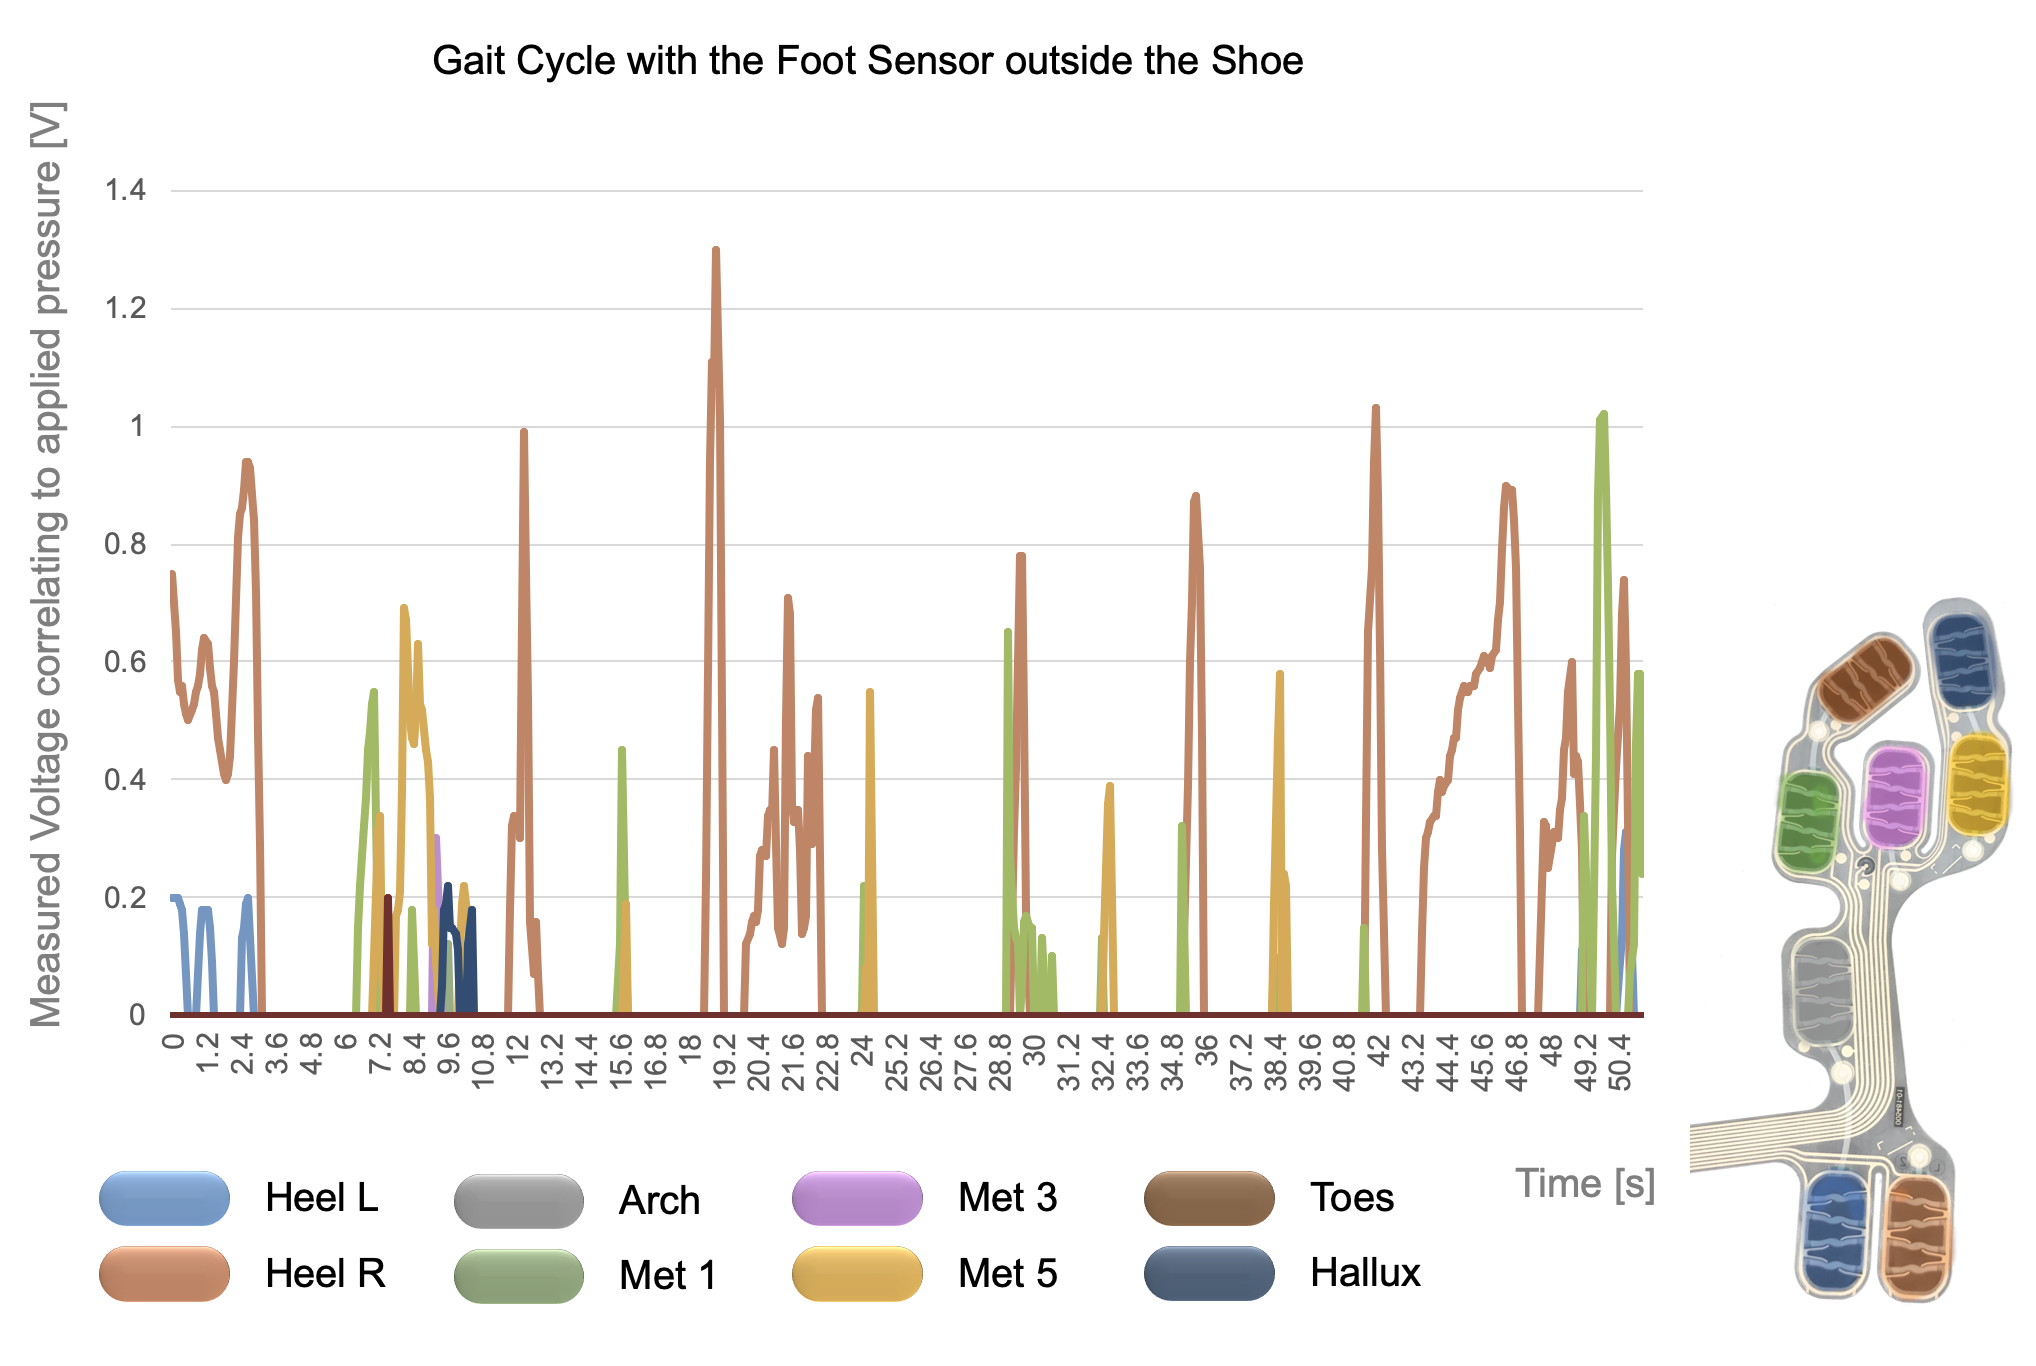
\includegraphics[width=1\columnwidth]{Images/Results/Gait_Cycle_3}
	\caption{\textbf{Measured values of a paraplegic pilot walking in the exoskeleton with the pressure sensor attached underneath the outer sole of the shoe.}}
	\label{Gait_Cycle_3}
\end{figure}
For the measurements inside the shoe a pattern corresponding to the step can be observed and the haptic feedback was implemented to be triggered at the moment the Metacarpal 3 sensor exceeds the threshold of 0.2 V.


\begin{enumerate}[\textit{1)}]
    \item{\textit{Evaluation of Haptic Feedback}}
\end{enumerate}

Due to the mentioned last-minute change in foot attachment from the shoe to the outer sole, it was not possible to test the developed haptic feedback properly. Therefore, the custom questionnaire was only partly filled with information. However, the results clearly show that the pilot S1 wishes for a stronger vibration through an alternative vibration motor or the combination of more than just one vibration motor triggered at the same moment.  \\
%%*************************************************************************
\begin{enumerate}[\textit{2)}]
    \item{\textit{Final Evaluation of the designs}}
\end{enumerate}
The evaluation was done with the SUS questionnaire.
The pilot S1 evaluated the ergonomic crutch and the length adjustment mechanism twice, an average score was then calculated. The haptic feedback and the VariLeg II crutch were only rated once by S1. The pilot S2 rated the ergonomic crutch, the VariLeg II crutch and the length adjustment mechanism once. The pilot S3 rated the ergonomic crutch design and the VariLeg II crutch once. The scores can be seen in fig. \ref{fig:SUS scores}.\\
The ergonomic crutch design, the length adjustment mechanism and the haptic feedback were evaluated separately, because they were not integrated into one whole system. For reference the VariLeg II crutch was evaluated as well. \\

\begin{figure}
    \centering
    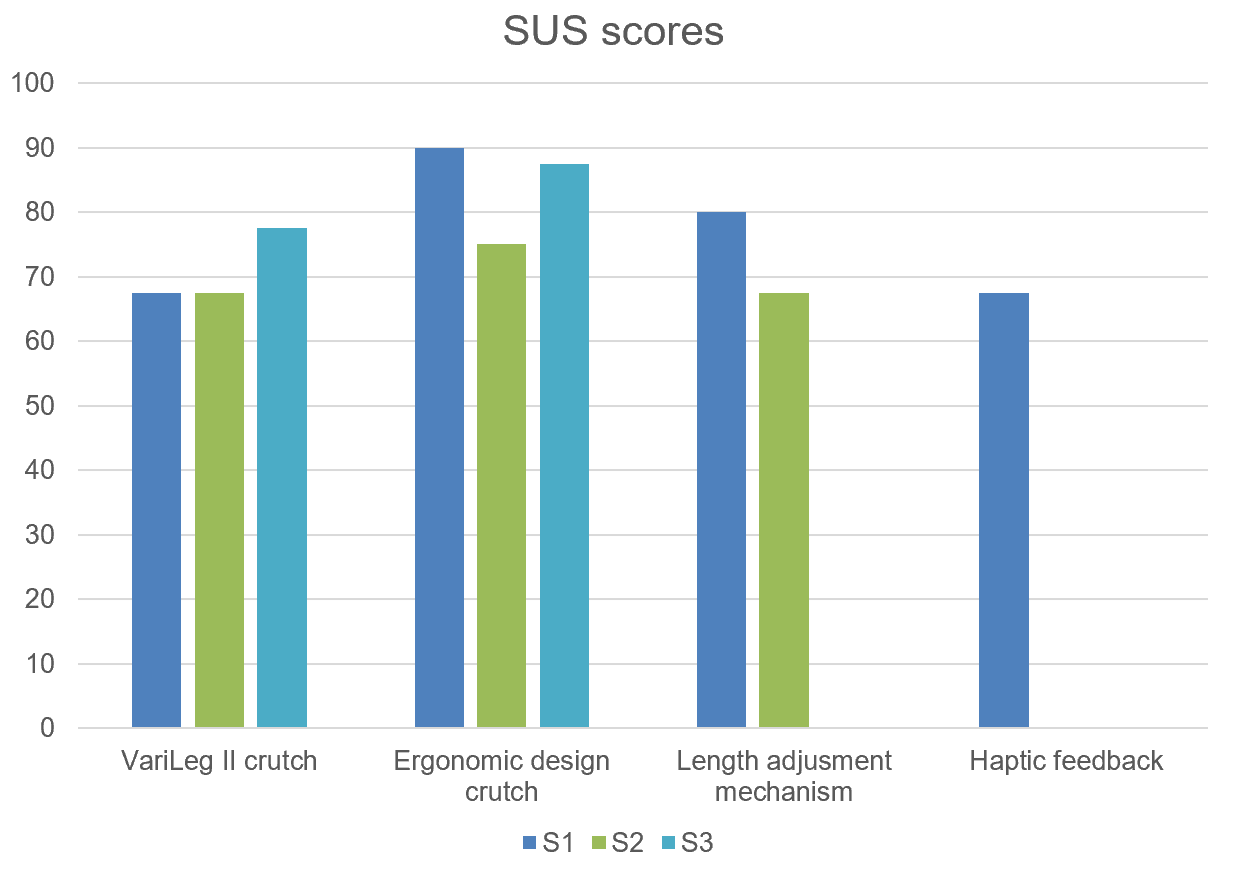
\includegraphics[width=1.0\columnwidth]{Images/Discussion/SUS_balkendiagramm.PNG}
    \caption{\textbf{Average SUS scores:} During evaluating SUS scores were defined. S1 evaluated the ergonomic crutch design and the length adjustment mechanism twice, all other assessments were done only once.}
    \label{fig:SUS scores}
\end{figure}





\section{Discussion}
Using the user-centered design method an individualized ergonomic crutch to control and maneuver the VariLeg enhanced exoskeleton was designed, focusing on one specific user. Two additional separate features, a length adjustment mechanism and a haptic feedback, were implemented independently from the control crutch and tested. An increase of usability of the ergonomic crutch design for the target population can be concluded as an overall improvement compared to the previous exoskeleton crutches was assessed by two novice paraplegic users and on experienced paraplegic user making use of subjective evaluation methods.


%SUS overall, Gewicht overall, werner findet auch unsere besser
%design nicht verallgemeinerbar
%sus limitierend, da hf als marginally acceptable angesehen
%es ist wichtig auch andere evaluationen anzuschauen bspw requirement vergleich --> requirement vergleich machen


\subsection{Analysis of Evaluation Results}
The crutches were evaluated with the system usability scale. The SUS is a standardized method to assess usability, thus the results can be used to compare different designs. 
All three users agreed independently, that the design of the VariLeg enhanced crutch surpasses the VariLeg II crutch in terms of usability. This would imply the user-centered design method to have achieved its intended purpose and improved the usability compared to a conventional developing method, as was done with the VariLeg II crutch. Due to lack of information to other instrumented crutches, we cannot compare the usability of designs.
It is also observable that so far the added features would not be improving the average score of the ergonomic crutch.
Not only designs can be compared together, but the SUS score can in general suggest if a product is well designed in terms of usability. A study from Bangor et al. \cite{bangor} compared SUS studies and suggested an adjective scale, which can be used to set SUS score in a context.
The scale was determined by comparing over 200 product studies with over 2000 filled questionnaires. Despite the original study was done with questions posed in English, the approach of comparing our results, which were translated in German, is taken to provide a framework for the result interpretation.\\
\\
The evaluation results are very impressive; however, they should be considered with caution due to the complexity of subjective perception. The effects of bias are considerable in the evaluation of the system. First of all, the pilot S1 was involved as user during every step of the process, which means that he is emotionally attached to the product. This makes it more difficult to give distinct feedback and impossible to evaluate objectively. Secondly, the solution is more intuitive for the user S1, if he helps design the product; therefore, we cannot conclude, that the solution would be applicable in further models or different users. Thirdly, the users character plays a big role in the nuances of the answers, e.g. one of our users only distinguished between “good” and “bad”. This led to answers only situated on one or the other end of the Likert scale. Causing an overall shift of the score to an extremely good one, even though the performance of the system might in reality have only been reasonably good.
The fact that the haptic feedback implementation achieves a marginally acceptable score, clearly reveals the limitations of the SUS evaluation method. The feature was only rated once and only by one pilot, therefore we assume the result to be depraved and not representative.\\

%in order to be able to compare results. The Ergonomic crutch design scored 90 on average for the experienced pilot and 87.5 for a novel user. The length adjustment mechanism scored 80 in average. The haptic feedback scored 67.5 on average and the VariLeg II crutch scored 77.5 for an experienced user and 67.5 for a novel user on average. \\

 


%\begin{figure}
    %\centering
    %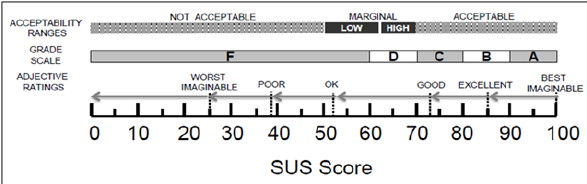
\includegraphics[width=1.0\columnwidth]{Images/Discussion/SUS_adjective-ratings.png}
   % \caption{SUS context}
    %\label{fig:SUScontext}
%\end{figure}
%Not only designs can be compared together, but the SUS score can in general suggest if a product is well designed. A study from Tullis and Albert compared SUS scores from 129 conditions with a wide range of subjects and found that the average SUS score was 66\% and the median 68\%.  The 25th percentile was 57 percent and the 75th percentile was 77 percent. \cite{tullisalbert} They concluded that an average SUS score below 60\% would suggest a poor performance, while over 80\% can be considered a pretty good value. This context indicates that the user-centered design worked well on the ergonomic crutch design, the length adjustment mechanism and the haptic feedback system.\\

\begin{figure}
    \centering
    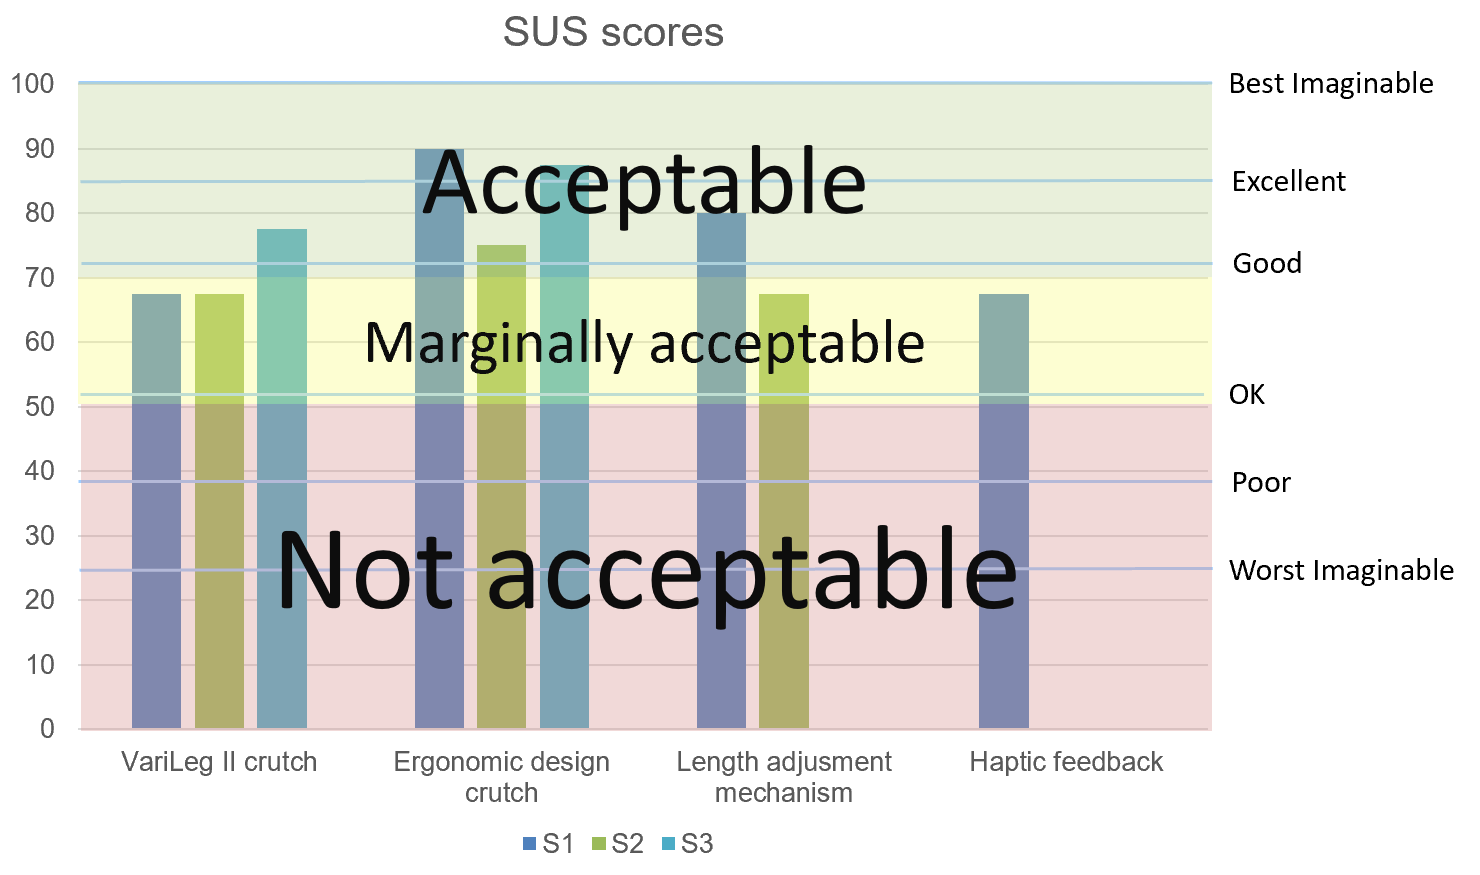
\includegraphics[width=1.0\columnwidth]{Images/Discussion/SUS_adjectives.PNG}
    \caption{\textbf{SUS scores in context:} The SUS score were set into perspective with the adjective scale established by Banogr et al.\cite{bangor}}
    \label{fig:SUSadjectives}
\end{figure}



\subsection{Requirement Comparison and Outlook}
The user evaluation methods showed limitations due to various factors, it is therefore important to simultaneously use an objective evaluation method. To address this the results were compared with the requirements set for the system.
In terms of the whole system, the goal of including two additional features to the control crutch was not achieved. The added features were not integrated into the whole system due to robustness issues, which have to be addressed first.
The weight goal of 1.5kg on the other hand was achieved on ease, the exact distribution can be seen in graph \ref{fig:weightgraph}.
\begin{figure}
    \centering
    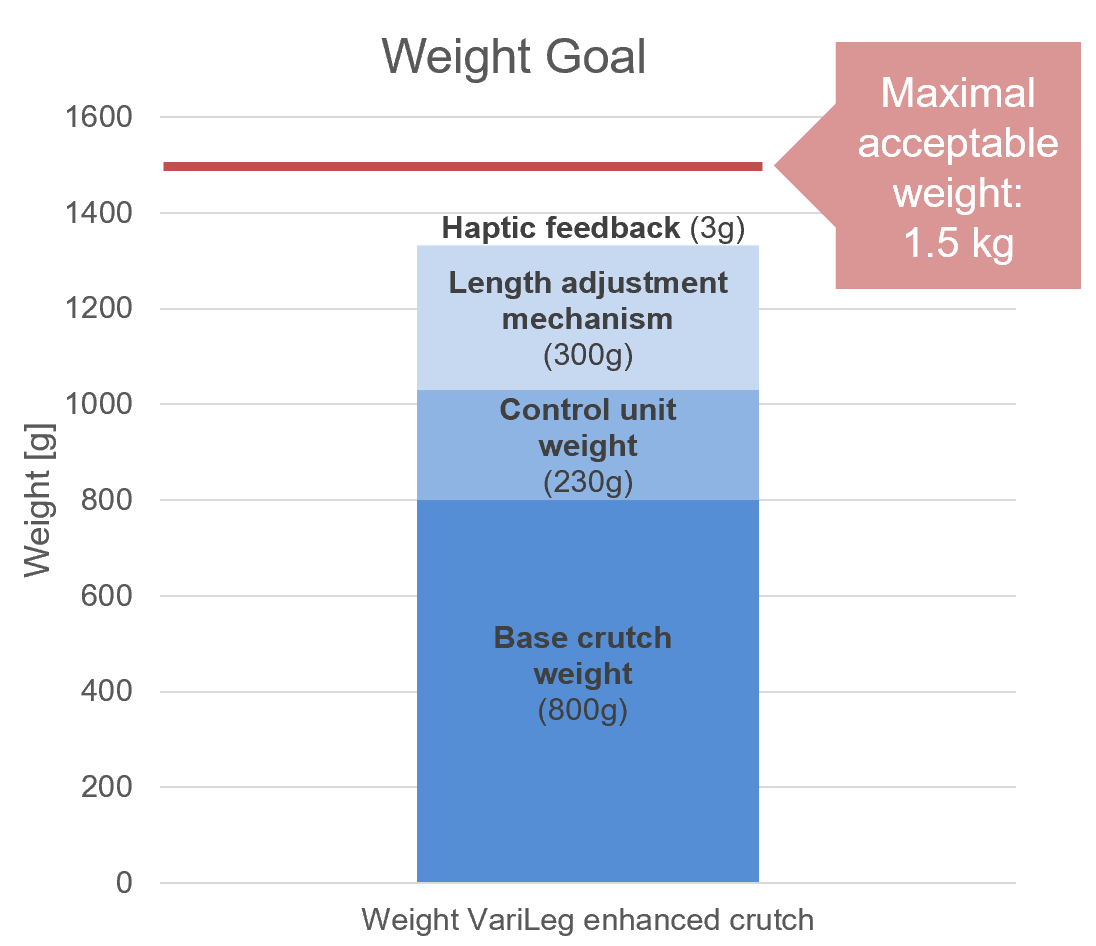
\includegraphics[width=1.0\columnwidth]{Images/Discussion/weightgraph.PNG}
    \caption{Weight distribution of the crutch}
    \label{fig:weightgraph}
\end{figure}
The "One Hand Free" feature was successfully implemented, the pilot is able to let the right crutch go and use his right hand to hold a railing or move objects.\\


\begin{enumerate}[\textit{i.}]
    \item {\textit{Ergonomic Crutch}}
\end{enumerate}

The ergonomic crutch design fulfils most of the requirements set in the defining phase. Only the left crutch is instrumented, the handle is ergonomic and the amount of buttons is kept to a minimum.
The crutch gives an overall positive impression in the evaluation; nevertheless, there are some key requirements not met concerning the usability that should be addressed.
The usability could be improved by designing the use of the modes more intuitive. Currently the pilot must remember the corresponding digit for ten different modes, which is difficult for the pilot and therefore a possible source for user mistakes. The problem could be faced for example with a larger display, which could show icons, like Project March \cite{projectmarch} does, to make the readability of the mode more intuitive. The probability of human error could also be reduced by preselecting the modes through computer vision obstacle recognition.
%Reducing the amount of separate modes and combining stair up and stair down mode to a single stair mode, where up and down can be divided with an additional up and down button or with step length settings, could improve the state as well.\\
%One of the main problems is the communication of the crutch with the exoskeleton. Due to a lack of time and knowledge no wireless communication channel was implemented, the signals are currently transmitted via a cable. The cable hanging from the crutch must be attached to the pilot’s arm with a Velcro band for it not to interfere with the system. This causes discomfort for the pilot.\\
During the CYBATHLON parkour the pilot is required to walk several steps between the obstacles, in order to conquer these as fast as and as laid back as possible continuous walking is essential. The ease of continuous walking could be improved if the pilot could already trigger the next step before the previous one is finished or use a continous walking mode.\\
%The pilot is not the only user of the crutch, the maintenance of the crutch should be simple for a good user experience by the technician. The current model of the crutch shows vast deficiency in this aspect. The space for the cables is too small to thread plugs through, this requires the cables to be soldered during assembly, which makes the disassembling and reassembling almost impossible.\\

\begin{enumerate}[\textit{ii.}]
\item{\textit{Length Adjustment System}}
\end{enumerate}

The mechanism for the dynamic length adjustment mechanism was newly designed despite of state-of-the-art solutions available for length adjustment, e.g. gas springs of office chairs. The main requirements were not met by any commercial solution, which required a completely new design.
The newly designed length adjustment mechanism fulfils the most important requirements: The system provides a locking mechanism at the end positions. The crutch can be shortened 15cm from the natural walking height. The extension mechanism is very fast and autonomously expands if triggered by the pilot.\\

The mechanism has proven itself to be very helpful to walk on the tilted path. The shortened crutch enables the pilot to walk upright and easily shift his weight according to the gait cycle.
The length adjustment mechanism seems very promising thanks to the fast extension mechanism of the crutches for standing up. The pilot can use the short crutches to push himself off the chair and extend them while straightening his legs. The fast extension ensures that the pilot does not lose balance while extending the crutches. The system did not work reliable enough during the first tests, therefore the pilot was depending on spotters help to keep balance while extending the crutches.
Initially the requirement was set, that the pilot could use the spring force to damp the speed of sitting down, but during testing the crutches appeared not to be helpful during sitting down. The trajectory of the exoskeleton is stable enough so the pilot S1 does not need the crutches at all during sitting down and the functionality is not needed.
The maximum spring force was reduced from 150N to 100N after the first tests. The pilot S1 found the collapsing of the crutches very cumbersome with 150N and the mechanism did not appear to be robust enough to withstand the big forces from the spring. Due to the fact, that the pilot does not need to damp the speed sitting down, the high forces did not show any benefits. \\
\\
The length adjustment mechanism in general seems very promising, but the mechanism lacks robustness and can therefore not be included to the control crutch before the issues are solved. The main problem were the pins, which didn't snap in reliable. This was mainly due to two reasons, first of all the clamp mechanism, which was only clamped around the crutch pipe startet slightly shifting, thus the pins were not perfectly aligned with the holes anymore. Secondly, the forces of the spring were to large and the slot started to enlarge, which caused a misalignment of the holes in the bottom and top crutch pipe. The problem could be addressed with a form fit of the clamp mechanism and dampers at the ends of the slot.\\

\begin{enumerate}[\textiit{iii.}]
\item{\textit{Haptic Feedback}}
\end{enumerate}

The complete integration of the haptic feedback into the use with a paraplegic pilot was unfortunately not possible, however many requirements were still met. The integration of the haptic feedback in the crutch module and the connection between the crutch module and the foot module worked reliably. The solution is minimally invasive due to the integration of the small vibration motor in the One-Hand-Free mechanism. The self-designed PCB for the ESP32 microcontroller in the foot module leads to an easy and compact integration of the foot pressure sensor. However, a wireless integration of the foot pressure sensor would enhance this integration even more. Even though tested in advance the pilot S1 did not recognize the vibration due to other distractions while walking. Therefore, the integration of more than one vibration motor or the change to a stronger one would be of interest. \\

One of the biggest challenges for the foot sensor was its placement. One must make sure that the weight of the pilot goes through the sensor, despite minor shifts in placement might already make big differences in the amount of force recognized by one sensor cell. Different settings where tried out, see app. \ref{subsec: HF different settings}. For the shoe attachement a reliable recognition of gait phases during walking was possible. However due to last minute changes on the foot attachment of the exoskeleton it was not possible to evaluate the haptic feedback, since the right placement in the outer sole shoe attachment turned out to be more challenging. Paddings on top of each sensor cell could help steering the flux of force through the cells. To avoid unwanted stresses on the cells through the pads, flexible pads are needed. Alternatively, to achieve a more reliable signal it could be preferable to include a calibration every time the exoskeleton is being started. This way small changes like the position of the pilot's feet and how strong the foot attachment is being tied would automatically be integrated into the code.  \\
We assume the difference in measurements of paraplegic and neurologically intact pilots are caused by the passive ankle module of the exoskeleton which does not produce a perfect roll off movement. However, the values read out of the specific sensor cells while the paraplegic pilot is walking in the exoskeleton correspond to a pressure which is around five times smaller than the peak values suggested by Soames \cite{soames1985foot} (using the typical response curve from app. \ref{subsec:HF Insole}.Therefore, further investigation on why the total amount of force recognized by the sensor is this low might help analyze the problem. A first draft of a calibration of the sensor was done for forces from 1 kg to 5 kg, however a closer analysis could be of interest. This way by adding up the different sensor cell voltages, it could be analyzed how well the PAS is working for if the percentage of the force going through the sensor is high then not all the weight of the pilot is carried by the exoskeleton and the pilot is indeed carrying some of his weight. \\


As soon as the right placement is found and a more robust signal can be read out more quantitative evaluation results could be achieved by using eye tracking methods in order to see whether the haptic feedback helps the pilot to stand more upright.\\ 



%%*************************************************************************

\section{Conclusion}
The user-centered design method was used to create an instrumented crutch to control and maneuver the VariLeg enhanced exoskeleton. The HRI was designed to meet the user S1 needs and two additional features, a dynamic length adjustment mechanism and haptic feedback corresponding the gait cycle, were added.
The implementation of the additional features showed an improvement in the user experience. The dynamic length adjustment mechanism was implemented in a fast and easy way, the solution does not add a lot of extra weight and does not need extensive modifications. The solution seems promising to be used for applications which must be weight effective.
The haptic feedback implementation shows potential for gait analysis applications and could be reused for other rehabilitation technologies for patients with gait weaknesses.
The user-centered design method helped to design a customized product for the user. The frame of the UCD method enhanced the addressing of specific user needs and might have helped rise the overall satisfaction rate. Due to the fact, that the method was focused on one specific user, we cannot in general conclude, that the method would show as good results for a large user group. 
The combination of different evaluation methods, like custom questionnaires and SUS, enabled us to consider more dimensions and alter between specific and wide perspective on the system. Therefore, we were able to cover more aspects, than with just one method. 
In general, we conclude it is very beneficial to involve the user through the whole design process of assistive devices, the product can be adjusted in numerous aspects through different phases to achieve a higher acceptance rate of assistive devices.\\



%%*************************************************************************

% use section* for acknowledgment
\section{Acknowledgment}
We would like to thank Prof. Dr. Roger Gassert for his valuable inputs and the opportunity to do the research for our bachelor thesis at the RELab. Likewise, we want to thank our supervisor Jan Meyer for his immeasurable support during our research and his critical questions. We thank Thomas Krieg for his relentless feedback and the numerous times of presence. We also thank Werner Witschi and Rolf Schoch for their constructive inputs. A special thanks goes to Bruno Kaufmann for his support and his manufacturing of components. We thank Durovis AG for sponsoring the springs for the length adjustment mechanism. We thank Miro Voellmy, Natacha Van Groeningen, Stefan Wick and Friedrich Rockenbauer for their constructive feedback. Finally, we want to thank the whole VariLeg enhanced team and the RELab research team for their continuous support.

\section{Contributions}
LT and XV designed the control unit handle. EB and LG set up the crutch code and built together the electronics of the control unit. LT and XV designed and evaluated the workshops, custom questionnaires and the SUS. TK, WW and RS gave critical feedback and evaluation to all the settings. LT designed the length adjustment mechanism. XV implemented the foot sensors and the haptic feedback.



%%***********************bibliography**************************************************

% trigger a \newpage just before the given reference
% number - used to balance the columns on the last page
% adjust value as needed - may need to be readjusted if
% the document is modified later
%\IEEEtriggeratref{8}
% The "triggered" command can be changed if desired:
%\IEEEtriggercmd{\enlargethispage{-5in}}

% references section

% can use a bibliography generated by BibTeX as a .bbl file
% BibTeX documentation can be easily obtained at:
% http://mirror.ctan.org/biblio/bibtex/contrib/doc/
% The IEEEtran BibTeX style support page is at:
% http://www.michaelshell.org/tex/ieeetran/bibtex/
%\bibliographystyle{IEEEtran}
% argument is your BibTeX string definitions and bibliography database(s)
%\bibliography{IEEEabrv,Bibliography/references}

% <OR> manually copy in the resultant .bbl file
% set second argument of \begin to the number of references
% (used to reserve space for the reference number labels box)
\bibliographystyle{IEEEtran}
% argument is your BibTeX string definitions and bibliography database(s)
\bibliography{IEEEabrv,Bibliography/references}









%\bibitem{IEEEhowto:kopka}
%H.~Kopka and P.~W. Daly, \emph{A Guide to \LaTeX}, 3rd~ed.\hskip 1em plus
%  0.5em minus 0.4em\relax Harlow, England: Addison-Wesley, 1999.
%

%%*************************************************************************

%BEGIN{RELAB} :: optional appendix (including datasheets etc.)
\cleardoublepage
%\onecolumn			%optional: switch to one column only (not recommended)
\appendix

\subsection{User-centered Design Method}
\subsubsection{Empathize}
\label{subsec:empathize}
\subsubsection{Define}
\label{subsec:define}

\begin{itemize}
    \item In order to define requirements for the crutches, the range of forces acting on the crutches during use by S1 were determined. The measurements were conducted with the VariLeg II crutches, which are equipped with force sensors. The data can be seen in fig. \ref{fig:forcesensordata}. The evaluation was done for following procedure twice: standing up, sitting down, standing up, walking some steps, sitting down. Peaks were determined to be around 400N. It can also be detected, that for sitting down the pilot loads the crutches with around 200N. The second time sitting down occurs at around 800s, the fourth time around 1150s. The first and third time sitting down can not be recognized due to the lack of reference data. 
\end{itemize}


\begin{figure}
    \centering
    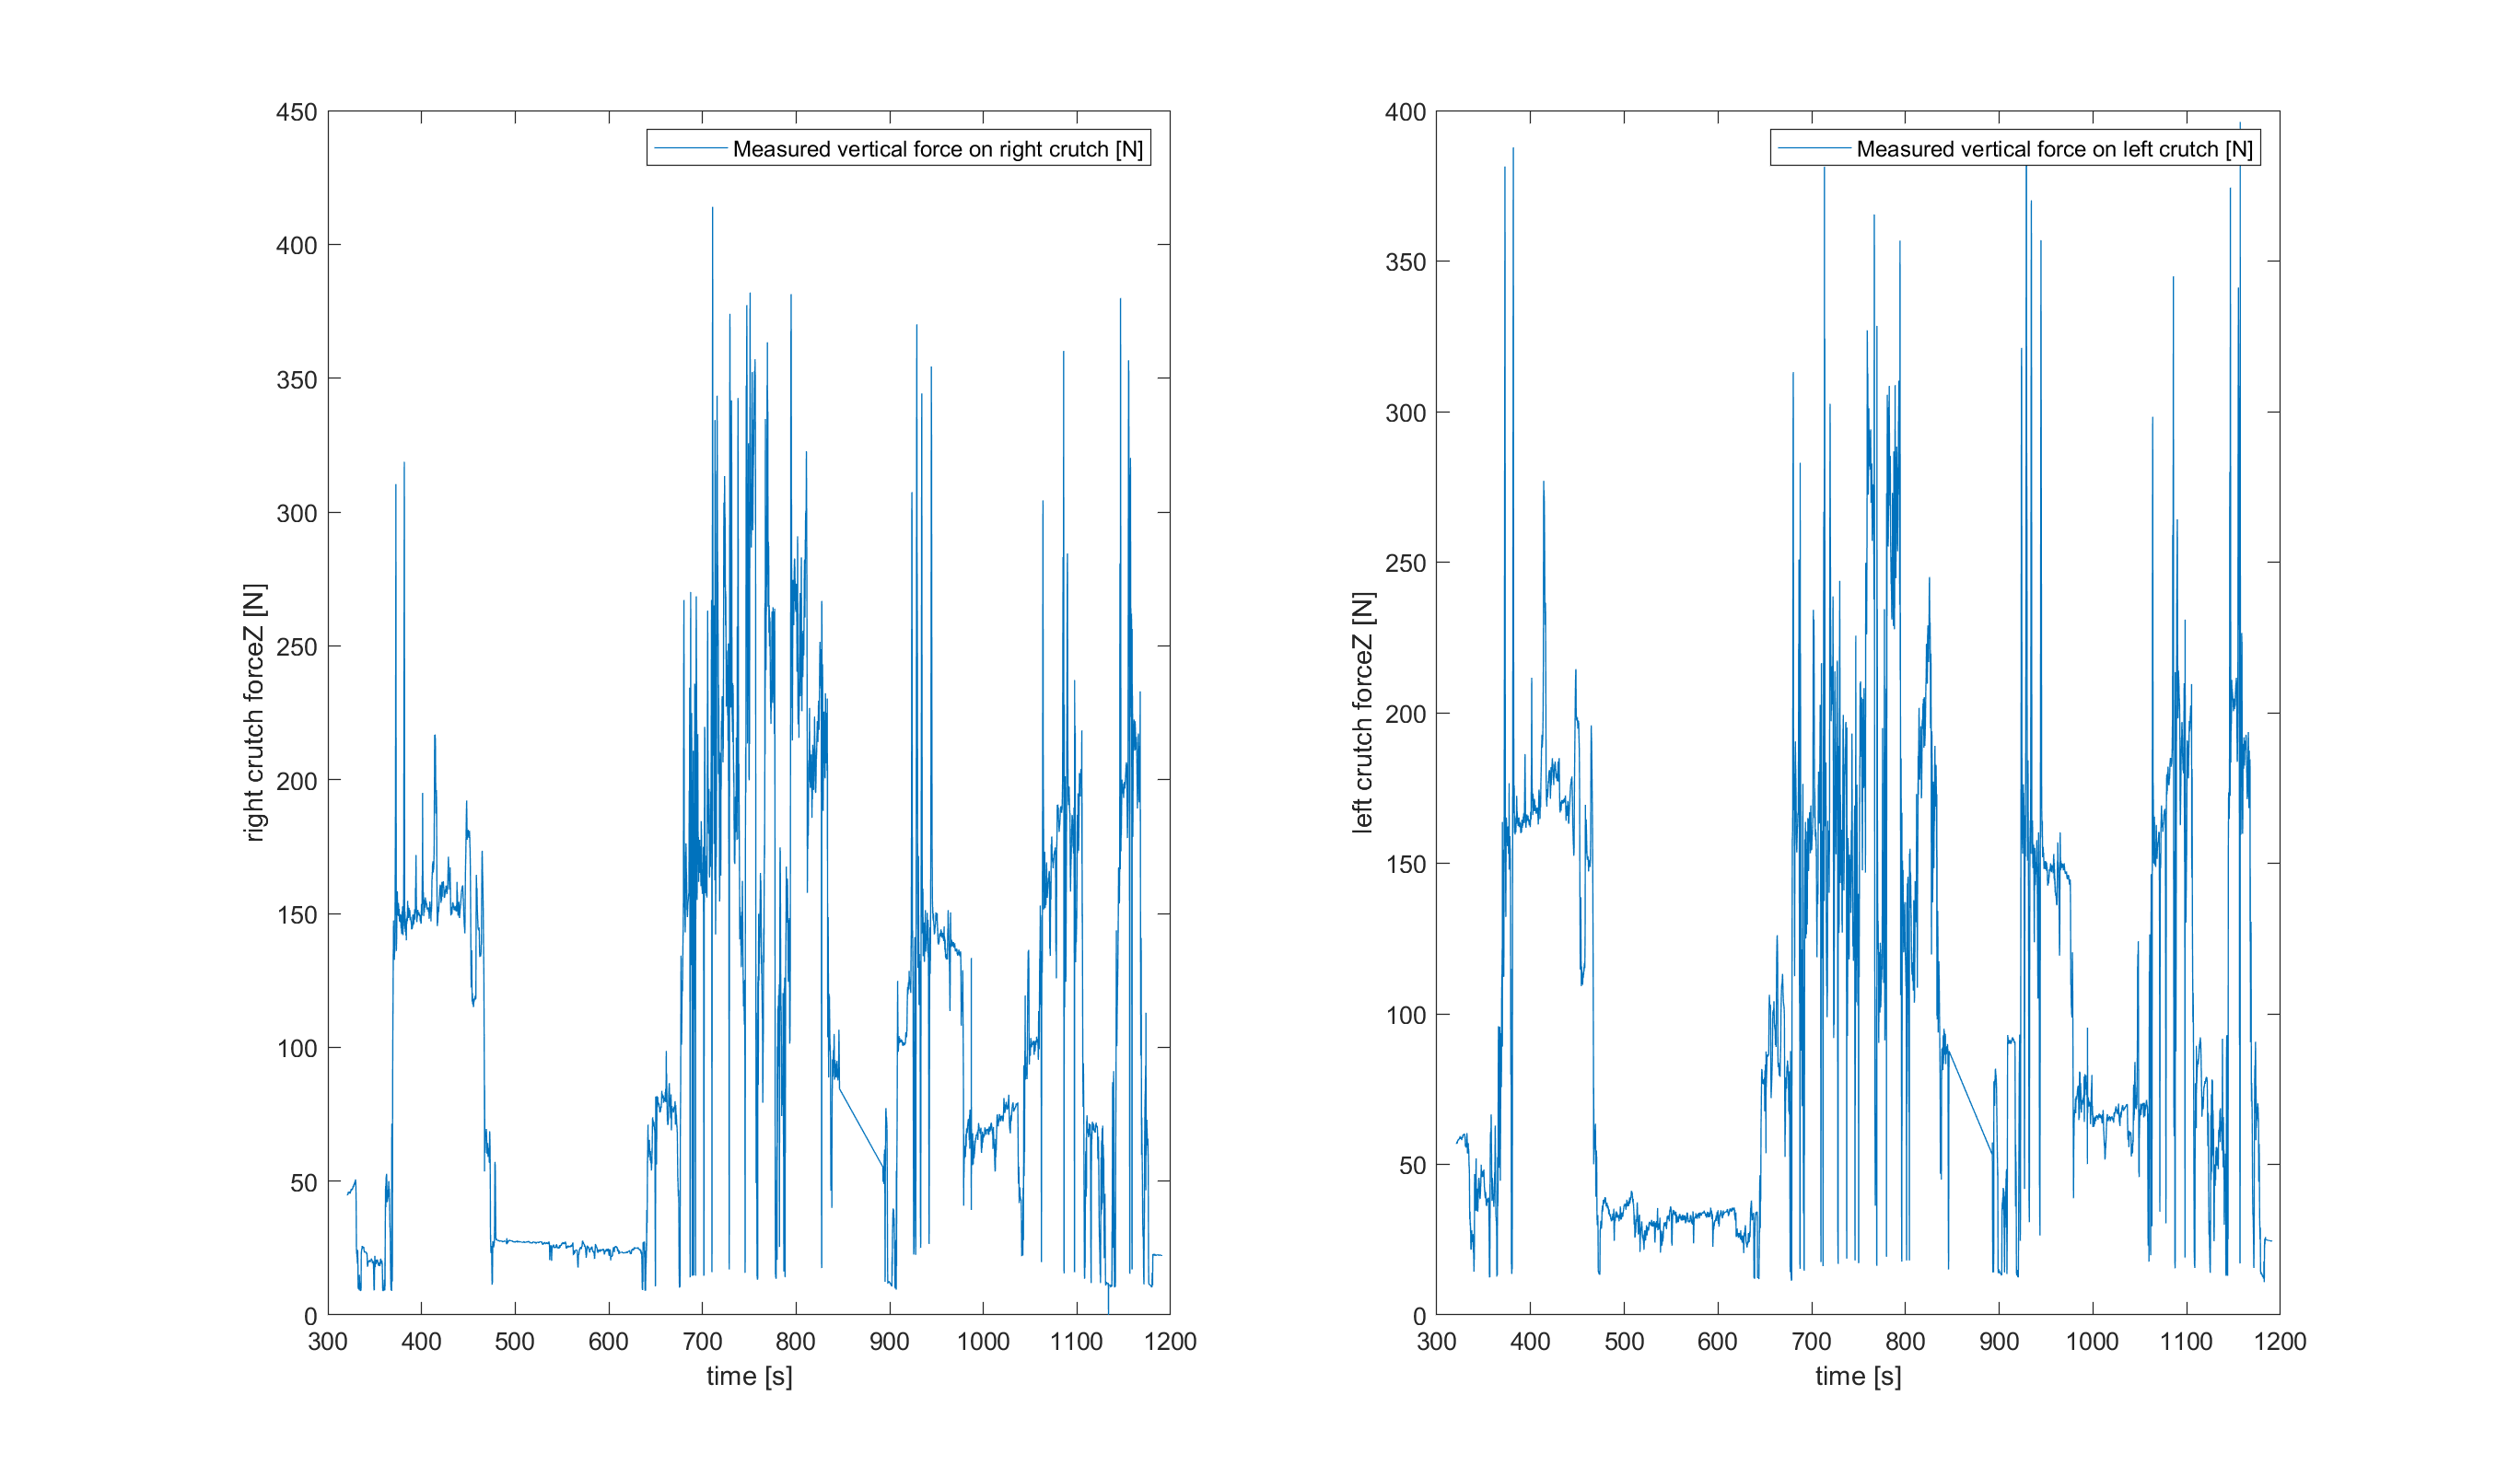
\includegraphics[width=1.8\columnwidth]{Appendix/ergonomic_crutch/forcesensordata.png}
    \onecolumn
    \caption[width=2\columnwidth]{\textbf{Measurements with force sensors:} To determine the load acting on the crutches during standing up, walking and sitting down. The pilot first gets up, sits back down, stands up again, walks some steps and sits back down. This was done twice, during the period from 830s until 890s the measurement was stopped. We can recognize peaks to lie at around 400N}
    \twocolumn
    \label{fig:forcesensordata}
\end{figure}


\subsubsection{Ideate}
\label{subsec:ideate}

\subsubsection{Prototype}
\label{subsec:prototype}

\subsubsection{Evaluate}
\label{subsec:evaluate}
For the evaluation of the different systems custom questionnaires and the system usability scale were used. The summaries of the different forms can be found here:\\
Custom Questionnaires: \textit{i. Ergonomic Crutch Design} \ref{pdf:EFB_EC}, \textit{ii. Length Adjustment Mechanism} \ref{pdf:EFB_LAM}, \textit{iii. Haptic Feedback} \ref{pdf:EFB_HF}, \textit{One Hand Free} \ref{pdf:EFB_OHF}\\
SUS: \textit{i. Ergonomic Crutch Design} \ref{pdf:SUS_EC}, \textit{ii. Length Adjustment Mechanism} \ref{pdf:SUS_LAM}, \textit{iii. Haptic Feedback} \ref{pdf:SUS_HF}, \textit{VariLeg II crutch} \ref{pdf:SUS_VLII}.
\cleardoublepage
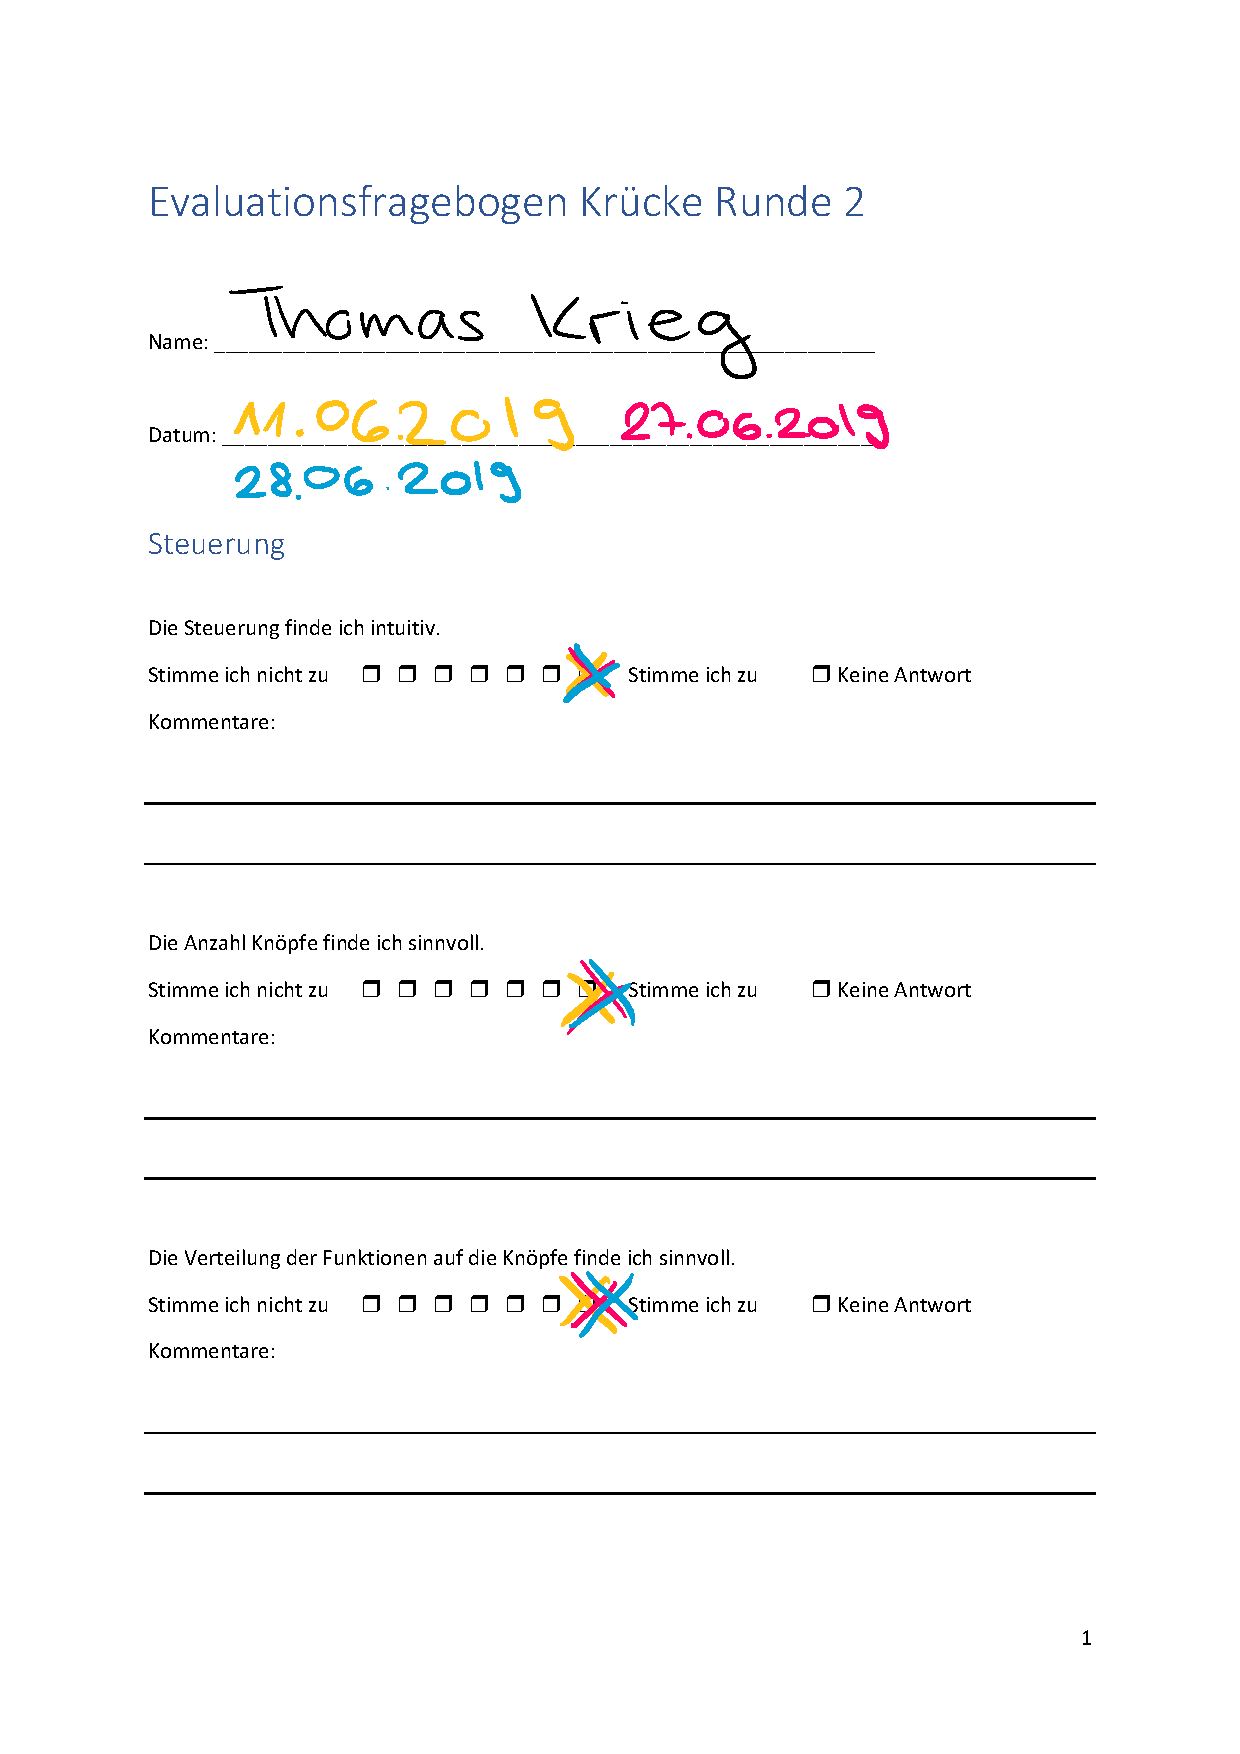
\includepdf[pages={1,2,3,4,5}]{Appendix/questionnaire/EFB_crutch_summary.pdf}
\label{pdf:EFB_EC}
\cleardoublepage
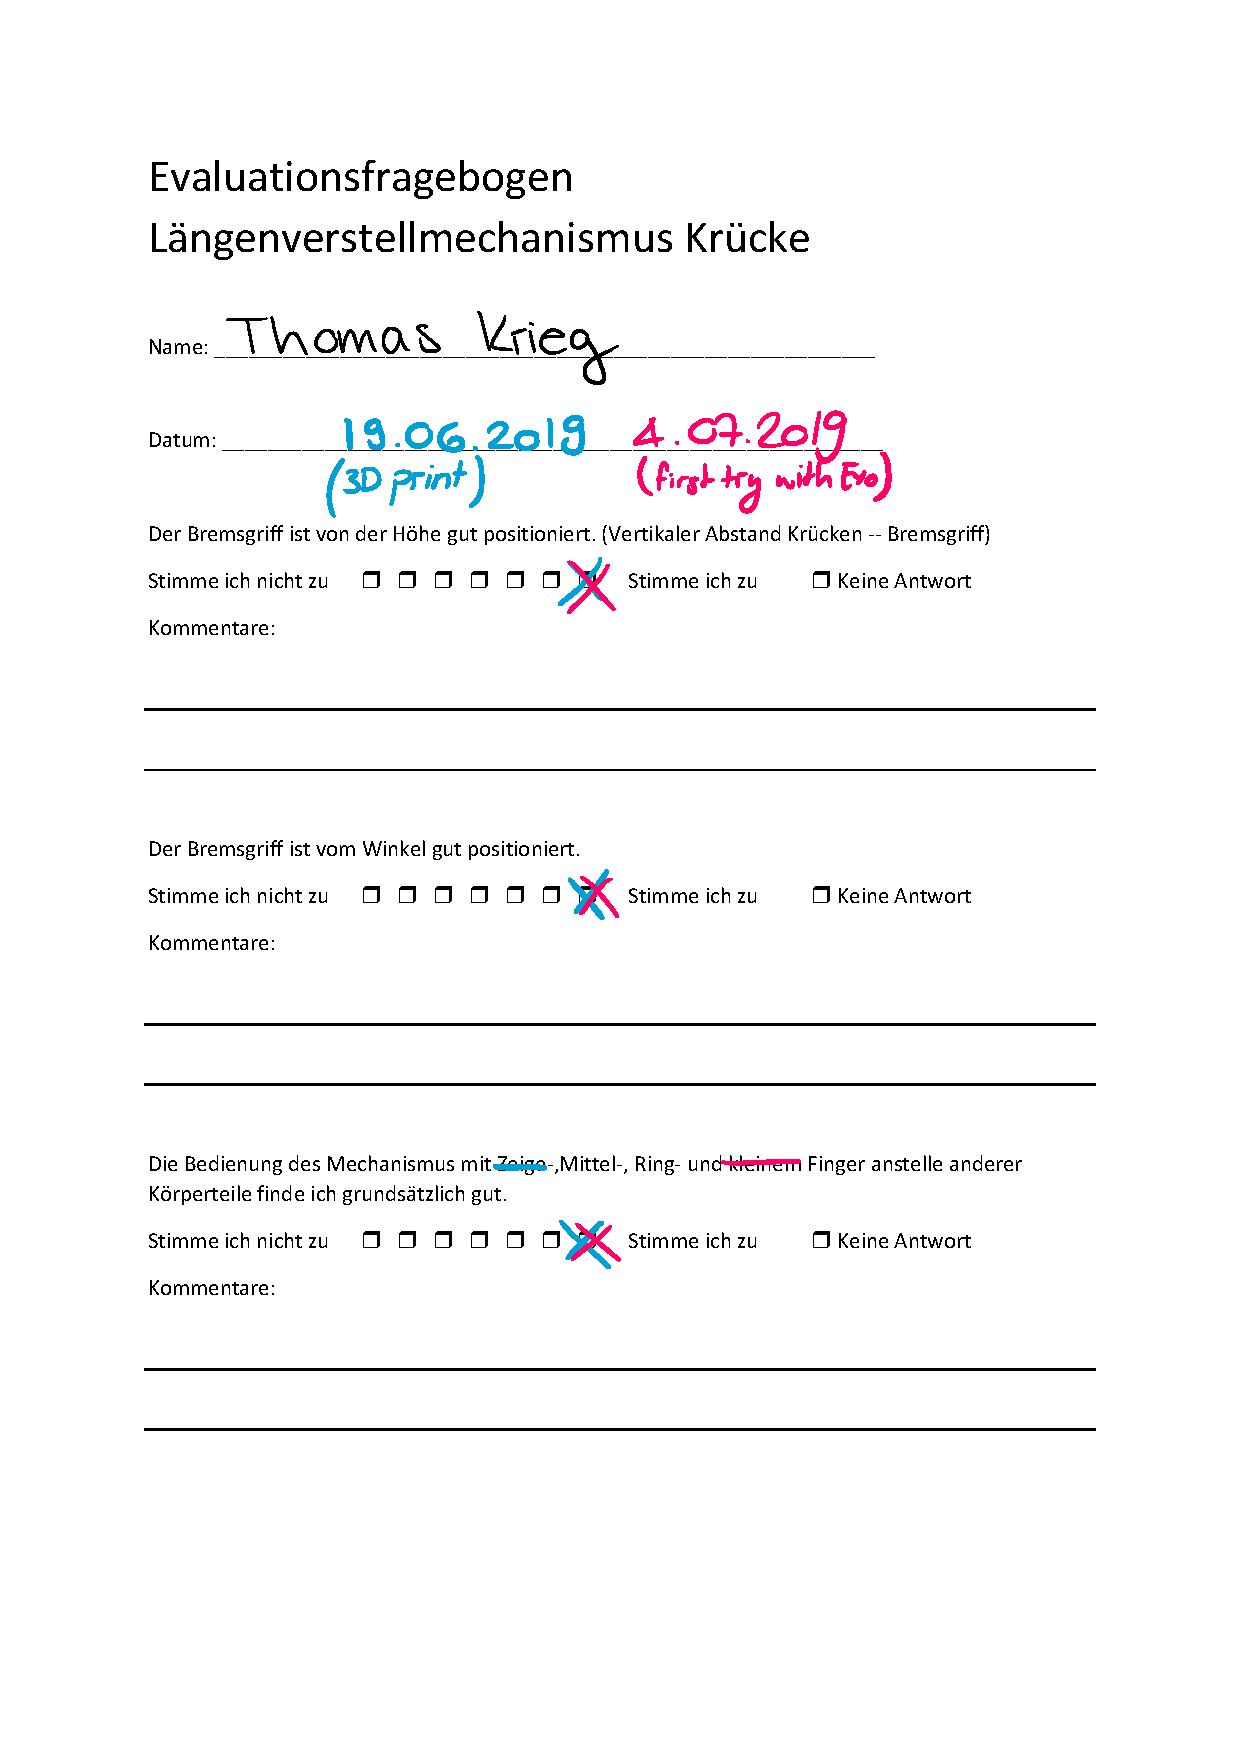
\includepdf[pages={1,2,3}]{Appendix/questionnaire/EFB_LAM_Summary.pdf}
\label{pdf:EFB_LAM}
\cleardoublepage
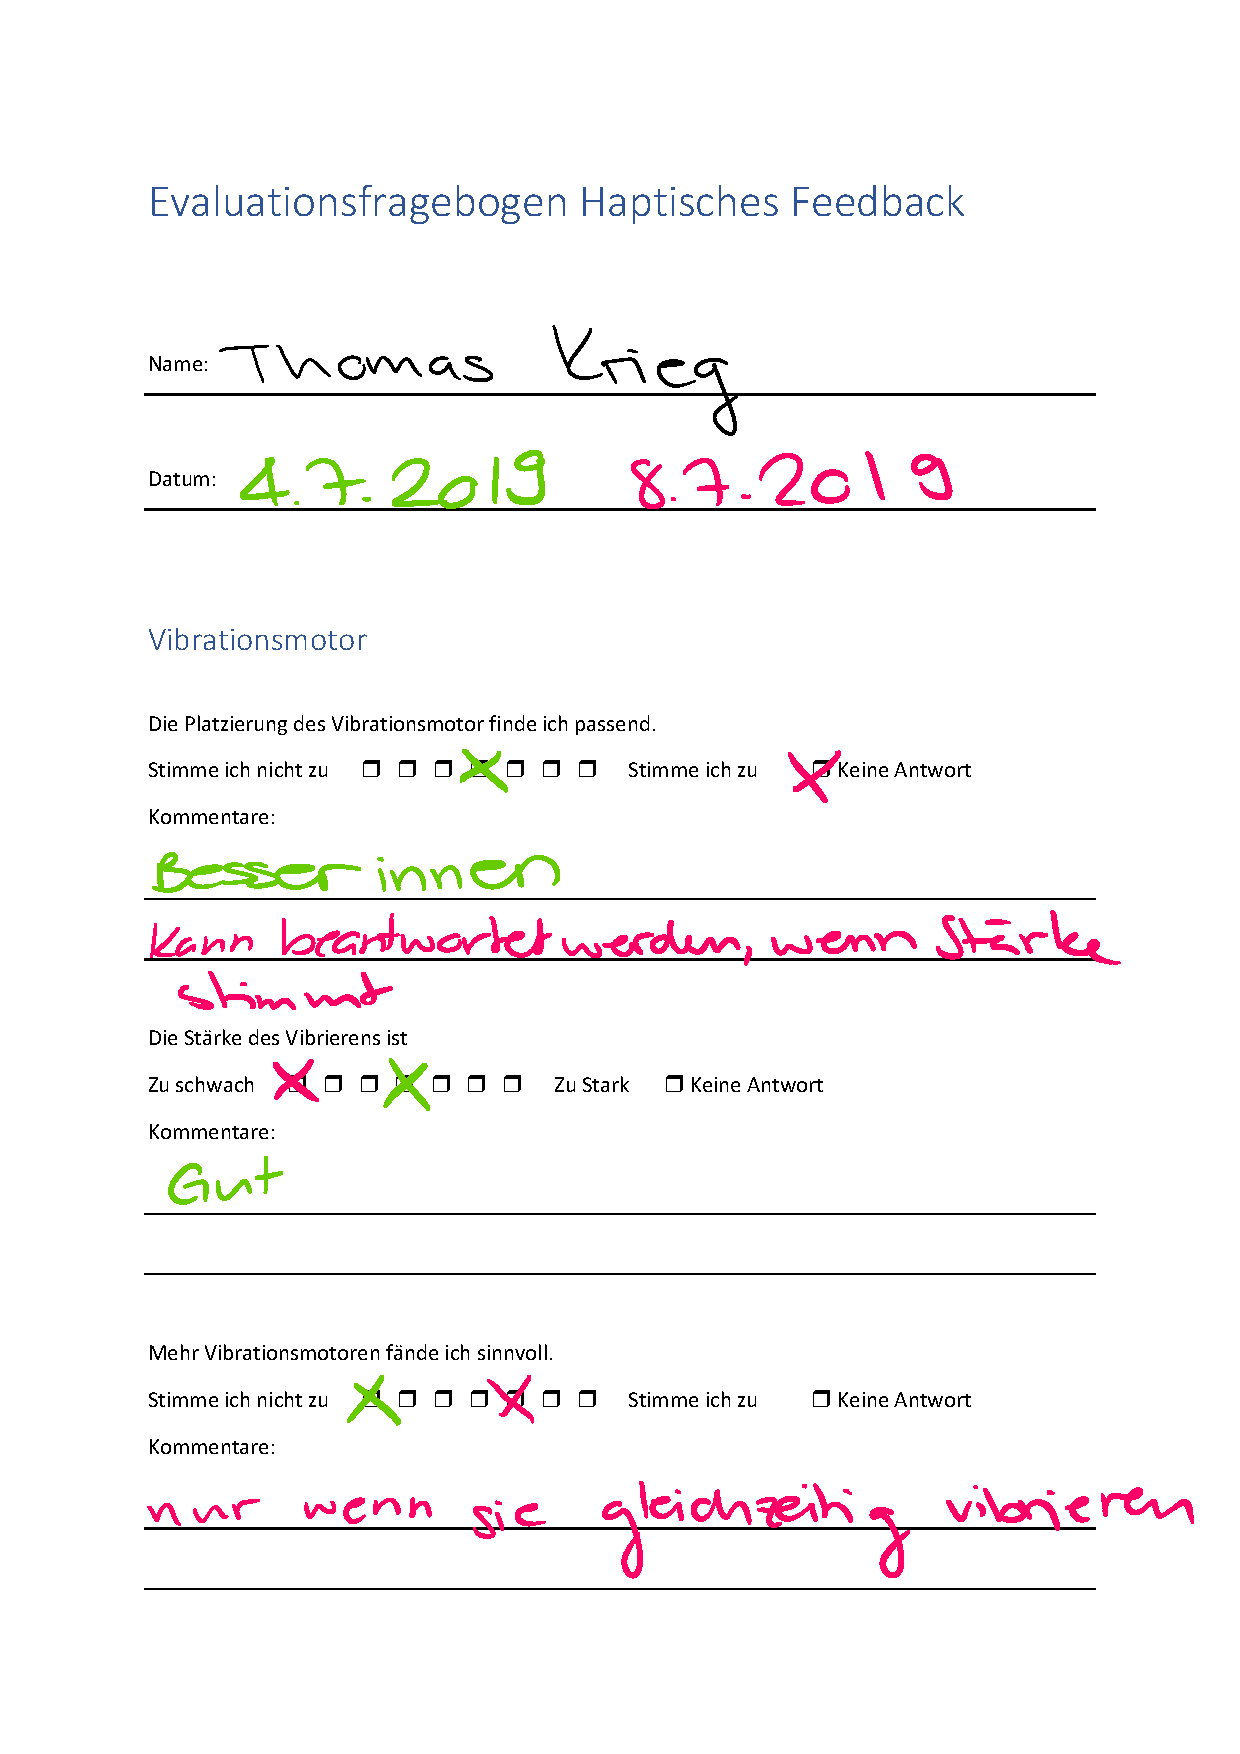
\includepdf[pages={1,2,3}]{Appendix/questionnaire/EFB_HF_Summary.pdf}
\label{pdf:EFB_HF}
\cleardoublepage
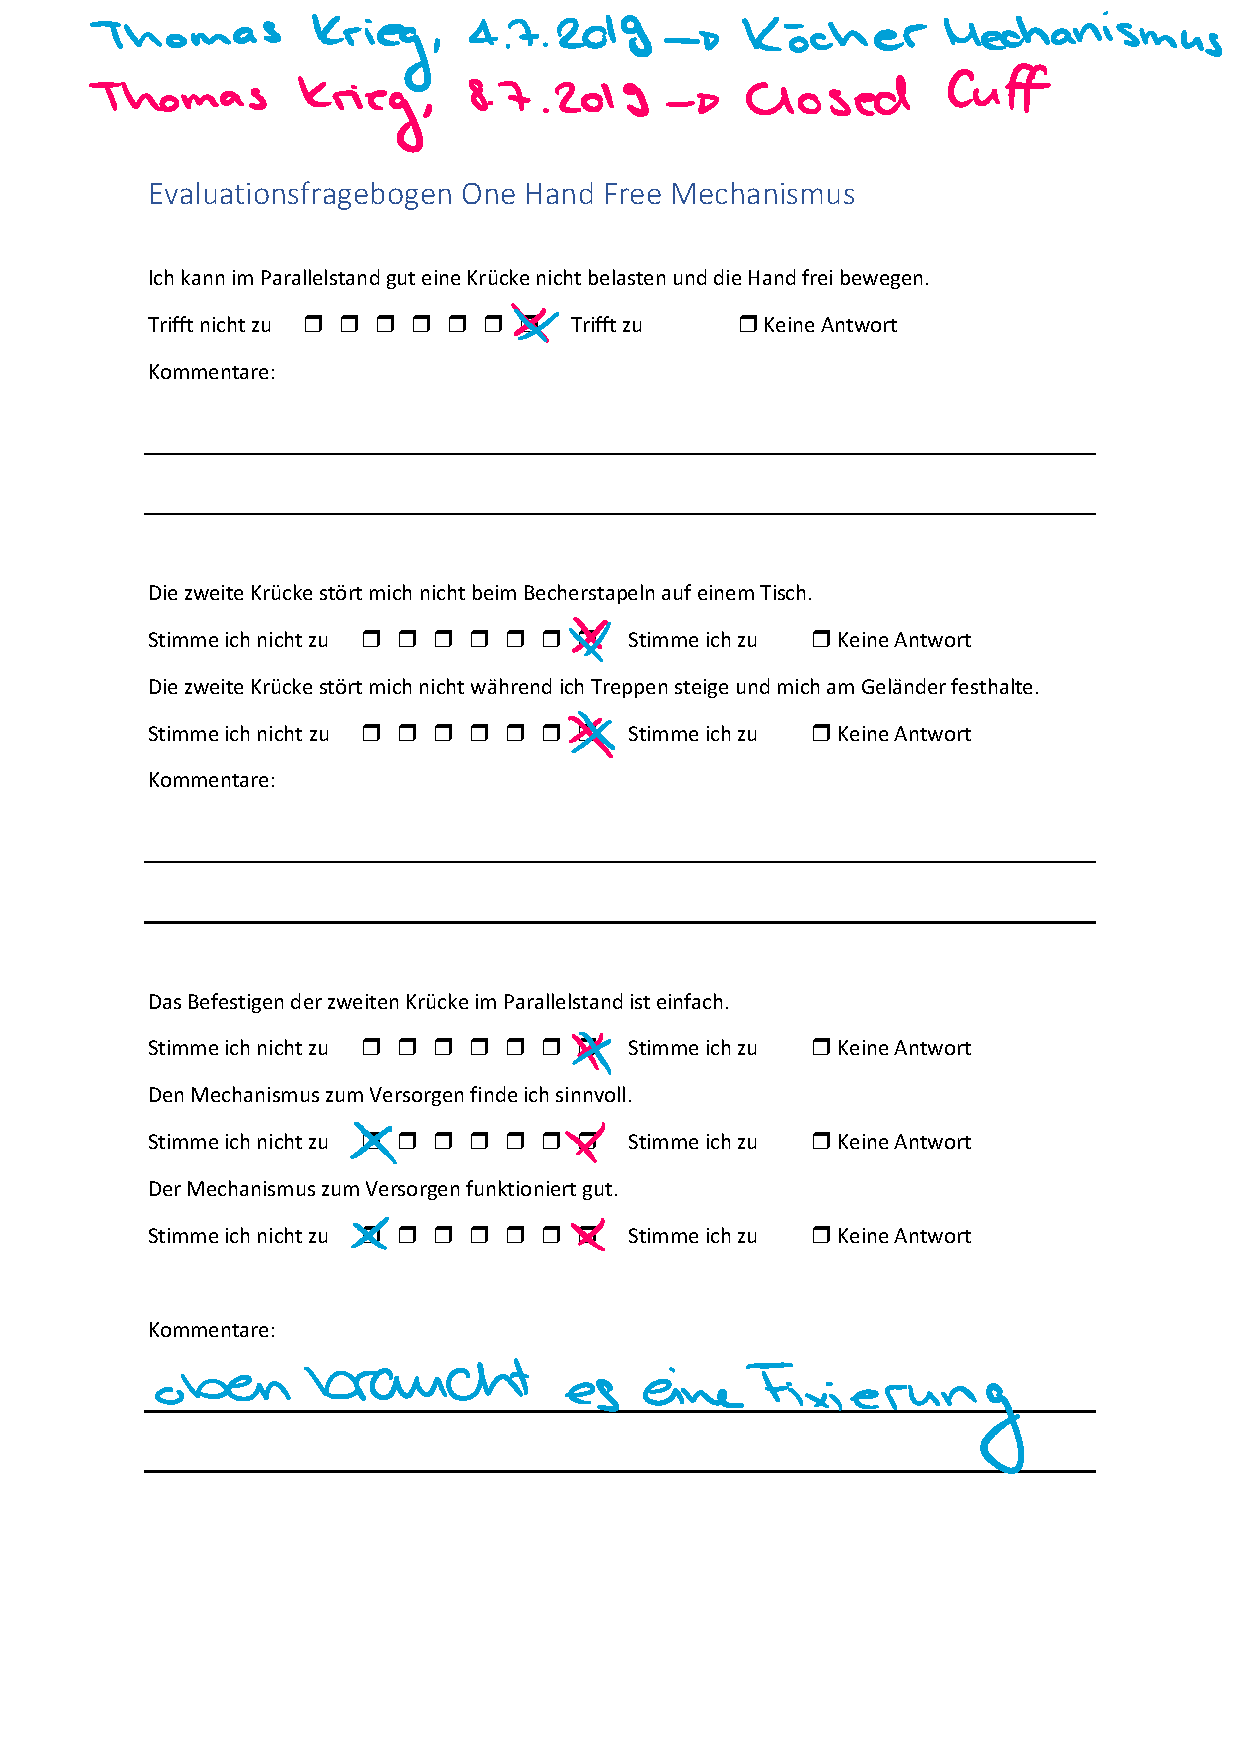
\includepdf[pages=1]{Appendix/questionnaire/EFB_OHF_Summary.pdf}
\label{pdf:EFB_OHF}
\cleardoublepage
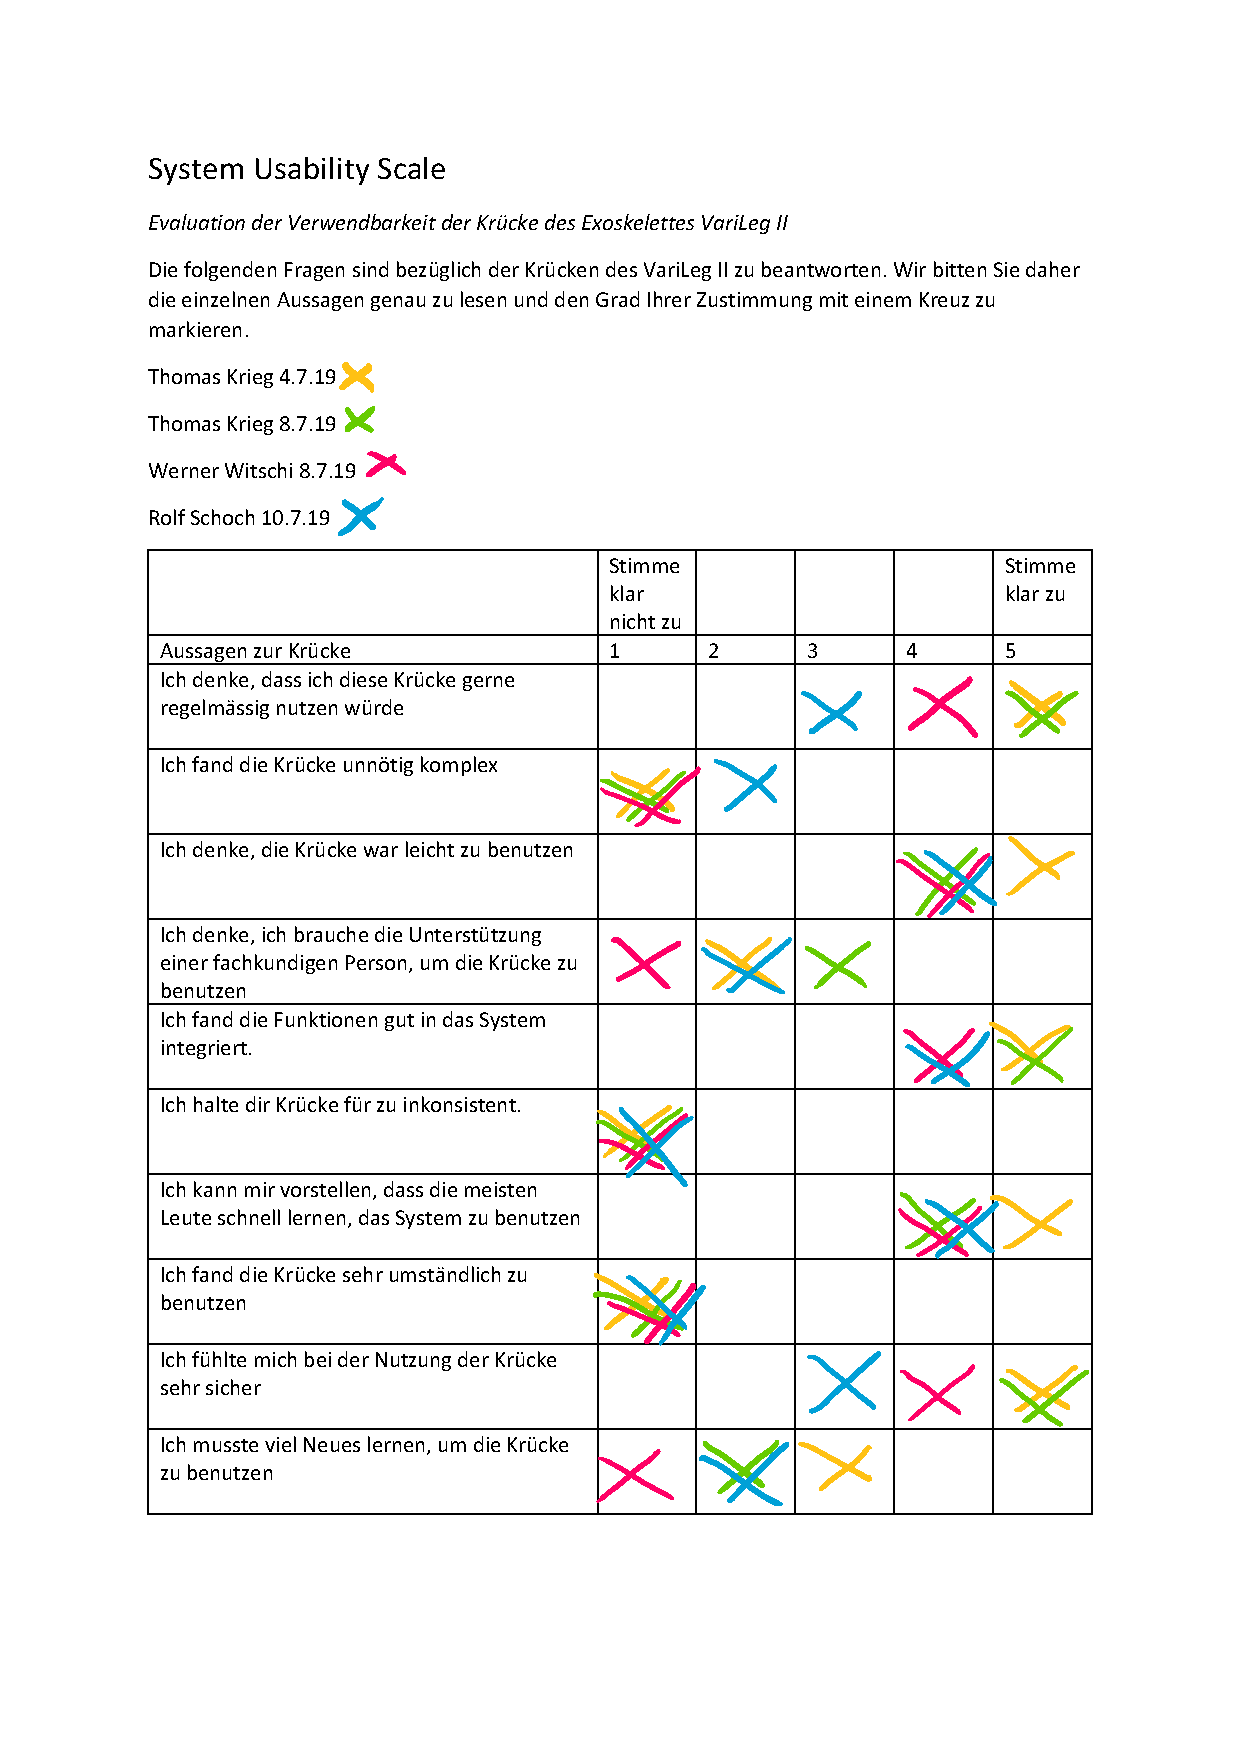
\includepdf[pages=1]{Appendix/questionnaire/SUS_EC.pdf}
\label{pdf:SUS_EC}
\cleardoublepage
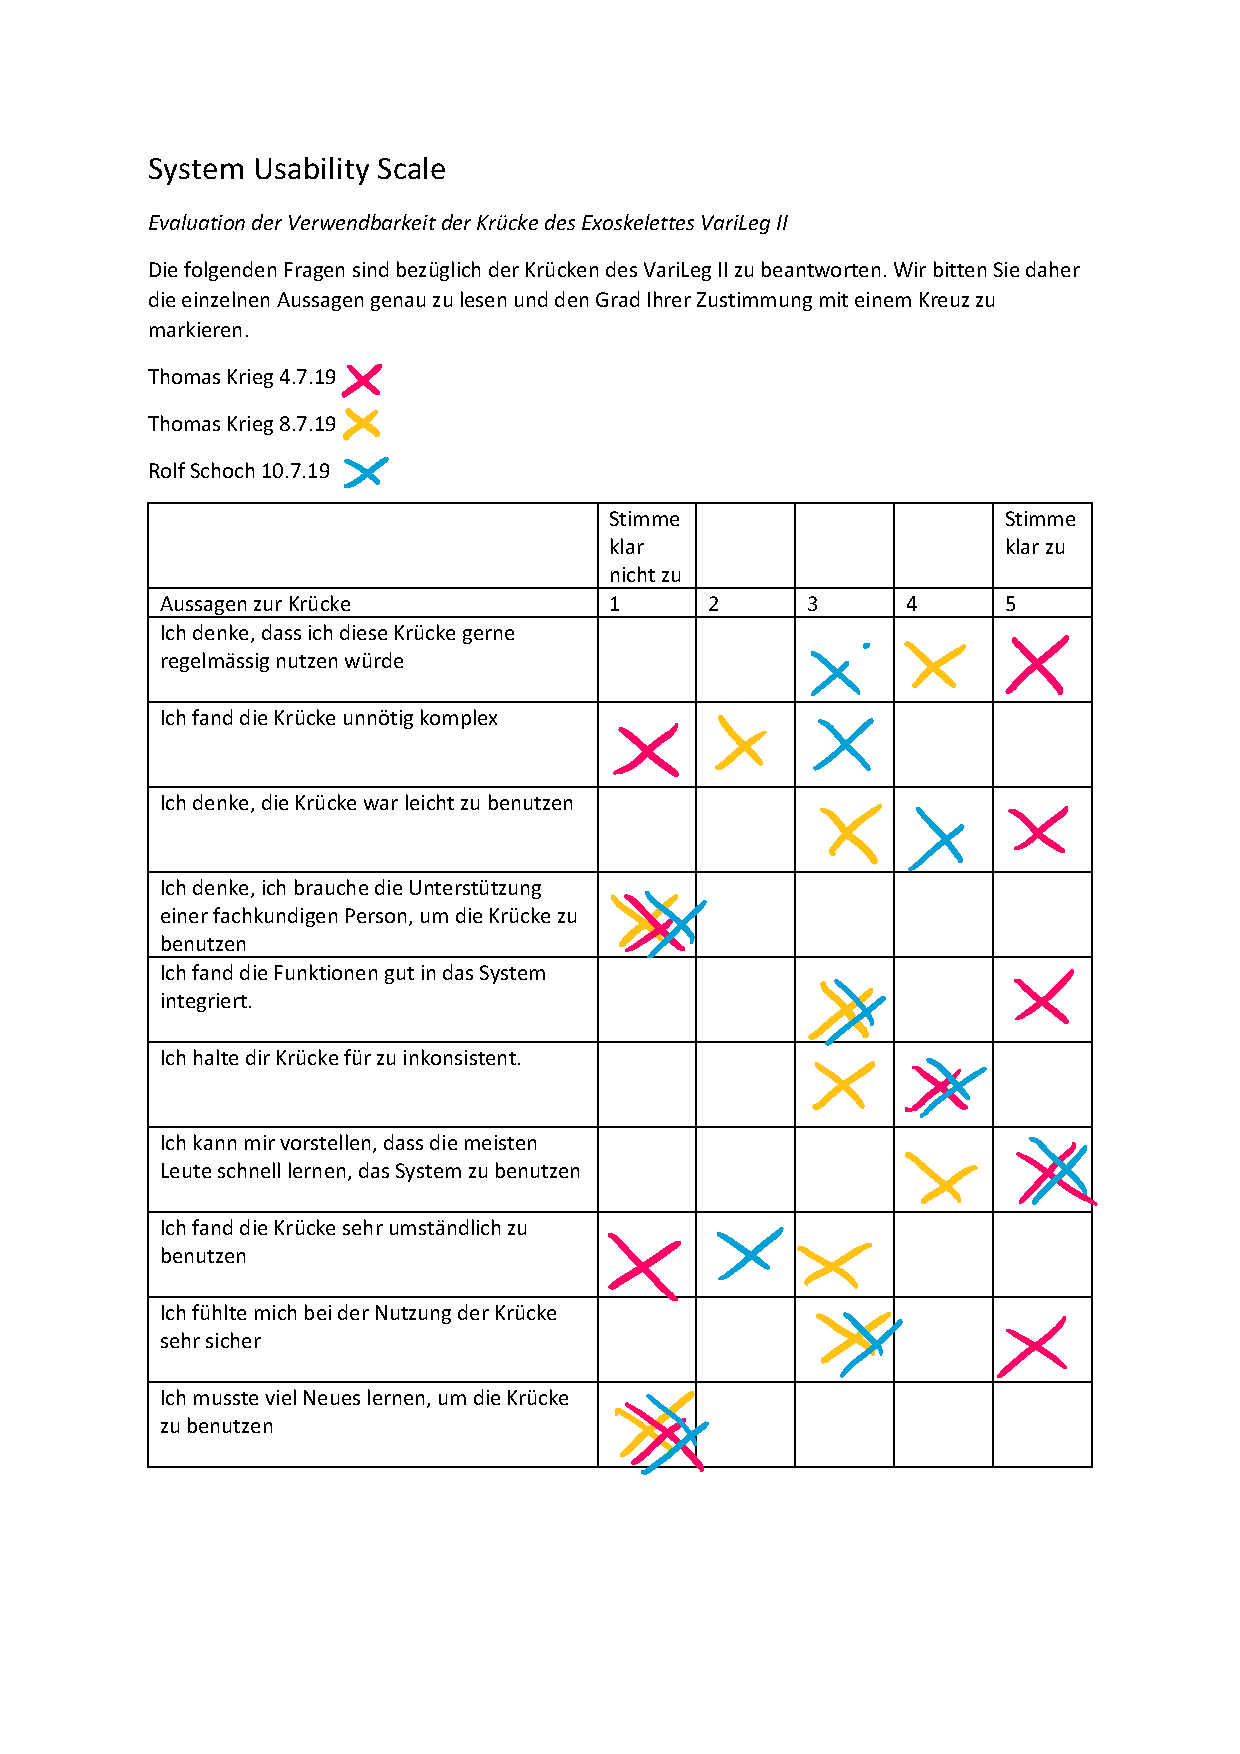
\includepdf[pages=1]{Appendix/questionnaire/SUS_LAM.pdf}
\label{pdf:SUS_LAM}
\cleardoublepage
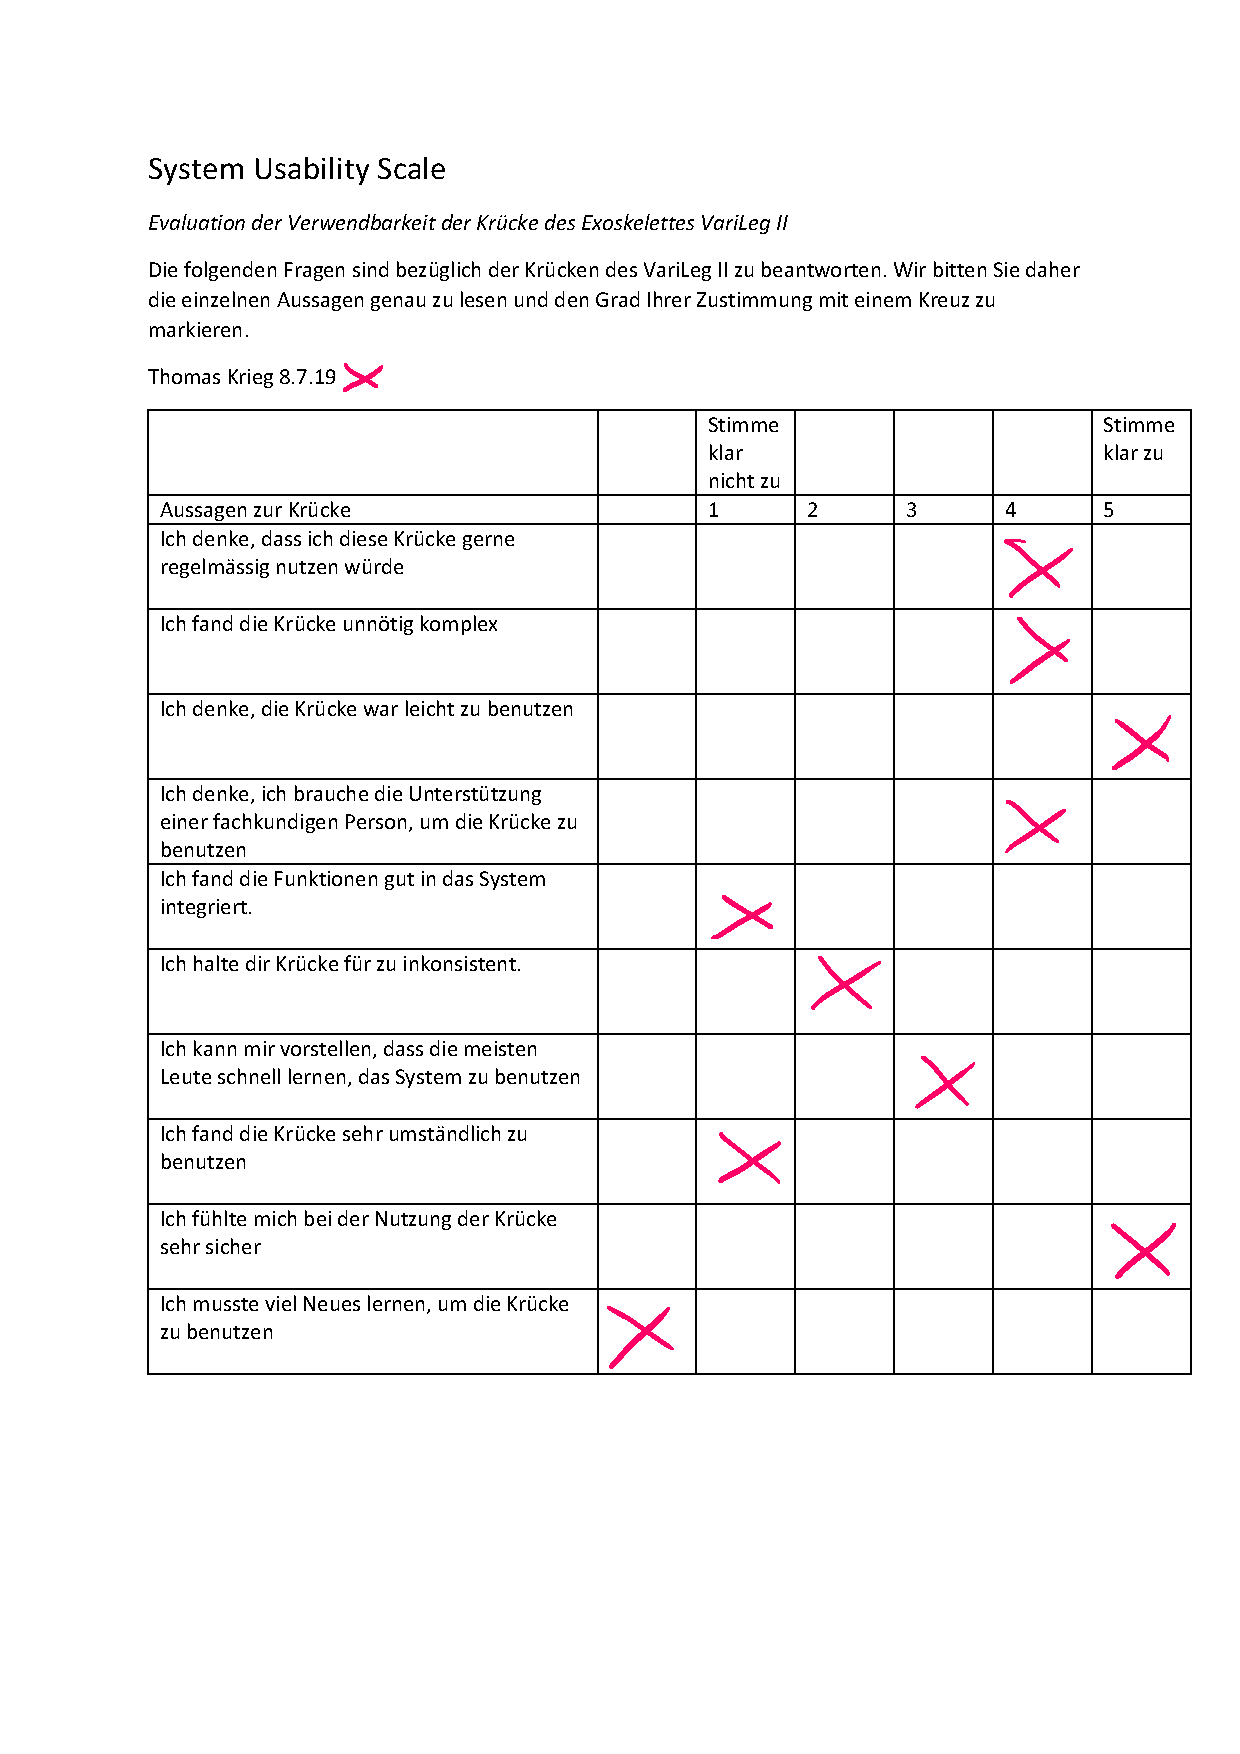
\includepdf[pages=1]{Appendix/questionnaire/SUS_HF.pdf}
\label{pdf:SUS_HF}
\cleardoublepage
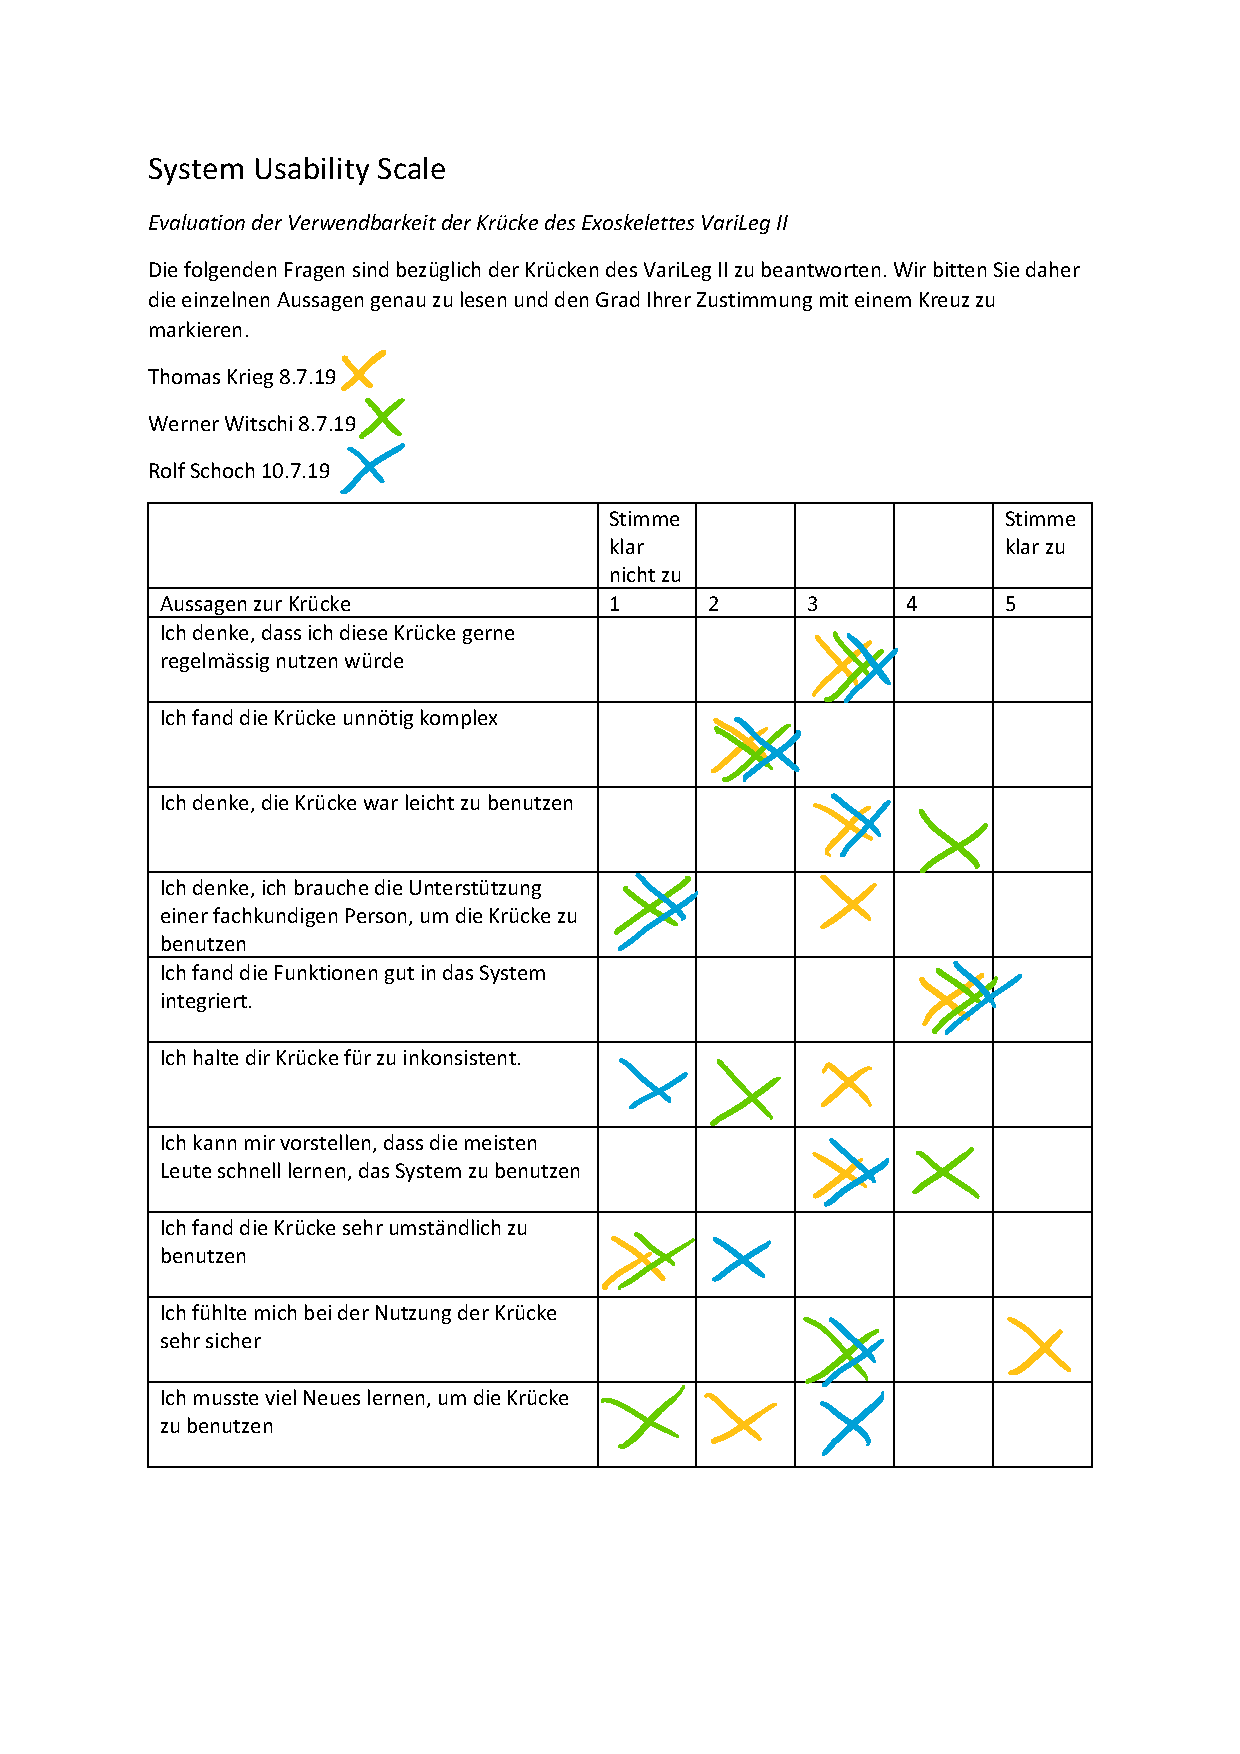
\includepdf[pages=1]{Appendix/questionnaire/SUS_VLII.pdf}
\label{pdf:SUS_VLII}



\begin{enumerate}[i.]
\item{Ergonomic Crutch Design}
\end{enumerate}

During User-Workshops first the requirements were discussed and then designs were established. The users had the possibility to integrate their design wishes into prototypes which were then modelled to achieve the first 3D printed prototype of the control unit.

\begin{figure}
    \centering
    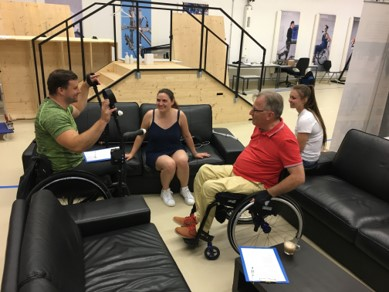
\includegraphics[width=1.0\columnwidth]{Appendix/User-centered_design_method/WS_Werner.jpg}
    \caption{Interviewing the former VariLeg II pilot and current VariLeg enhanced pilot}
    \label{fig:interview}
\end{figure}
\begin{figure}
    \centering
    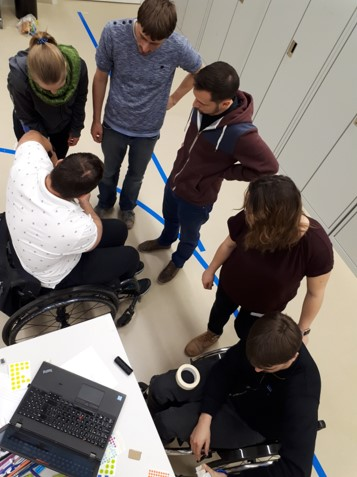
\includegraphics{Appendix/User-centered_design_method/WS_Rolf.jpg}
    \caption{Workshop environment with the pilots}
    \label{fig:ws_up}
\end{figure}
\begin{figure}
    \centering
    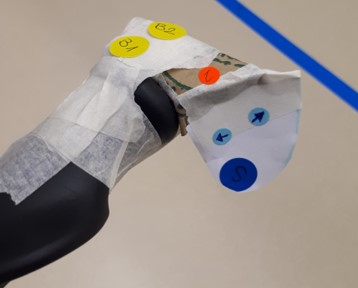
\includegraphics{Appendix/User-centered_design_method/WS_Karton.jpg}
    \caption{Handicrafted control unit design}
    \label{fig:handicraft}
\end{figure}
\begin{figure}
    \centering
    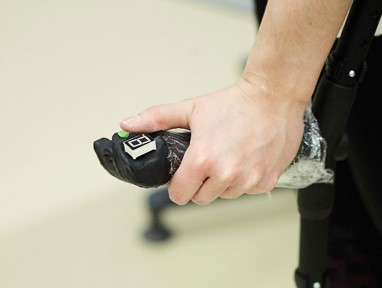
\includegraphics{Appendix/User-centered_design_method/WS_Fimo.jpg}
    \caption{Handicrafted control unit design}
    \label{fig:handicraftfimo}
\end{figure}
\begin{figure}
    \centering
    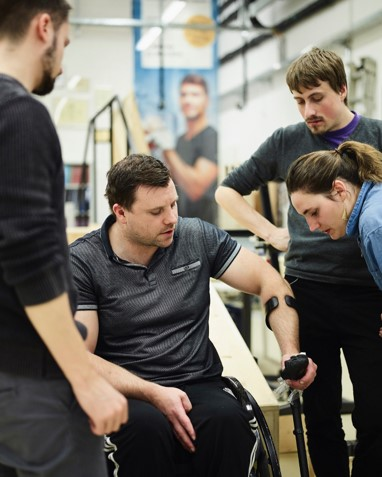
\includegraphics{Appendix/User-centered_design_method/WS_EKZ.jpg}
    \caption{Discussing the design}
    \label{fig:ekz}
\end{figure}
\cleardoublepage
\label{subsec:Ergonomic Design}

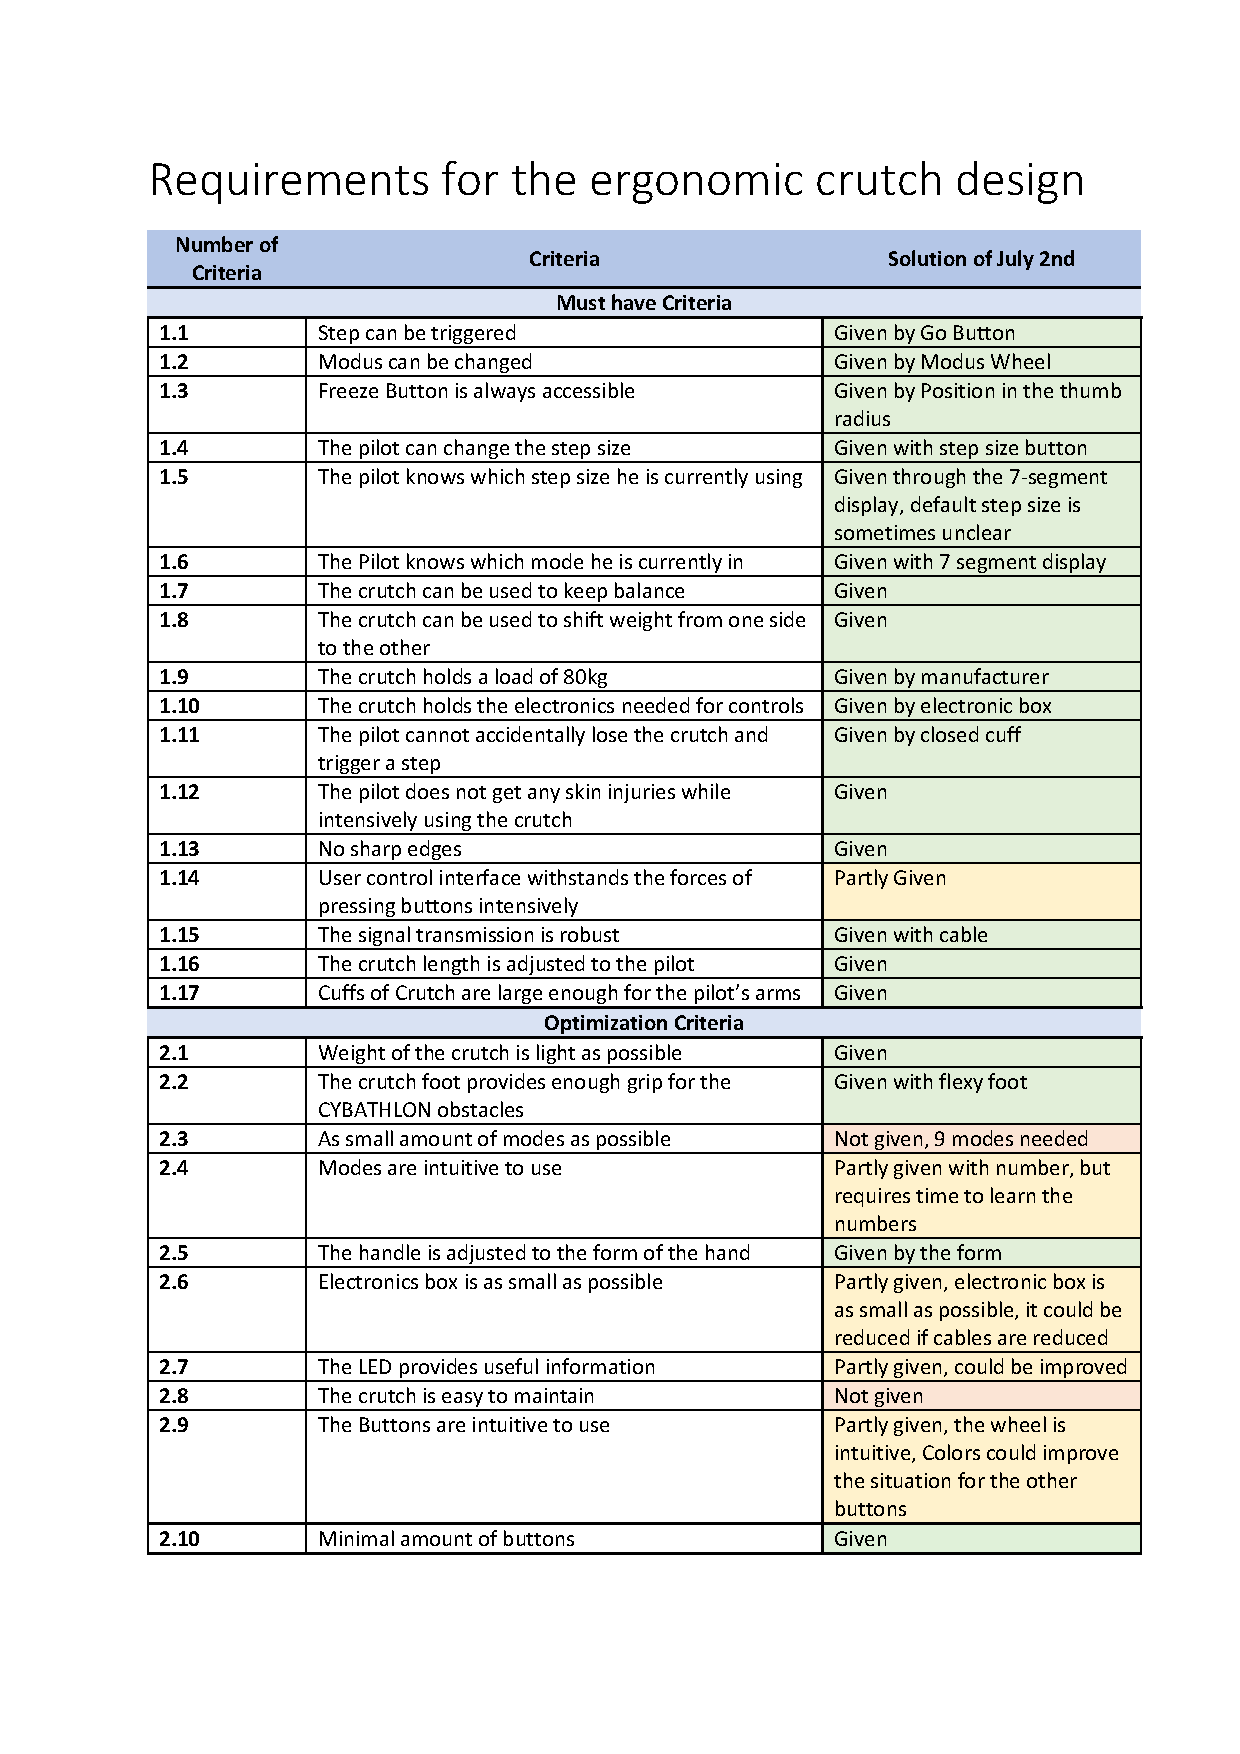
\includepdf[pages=1]{Appendix/ergonomic_crutch/Requirements_ergonomic_crutch.pdf}
\label{subsec:EC requirements}
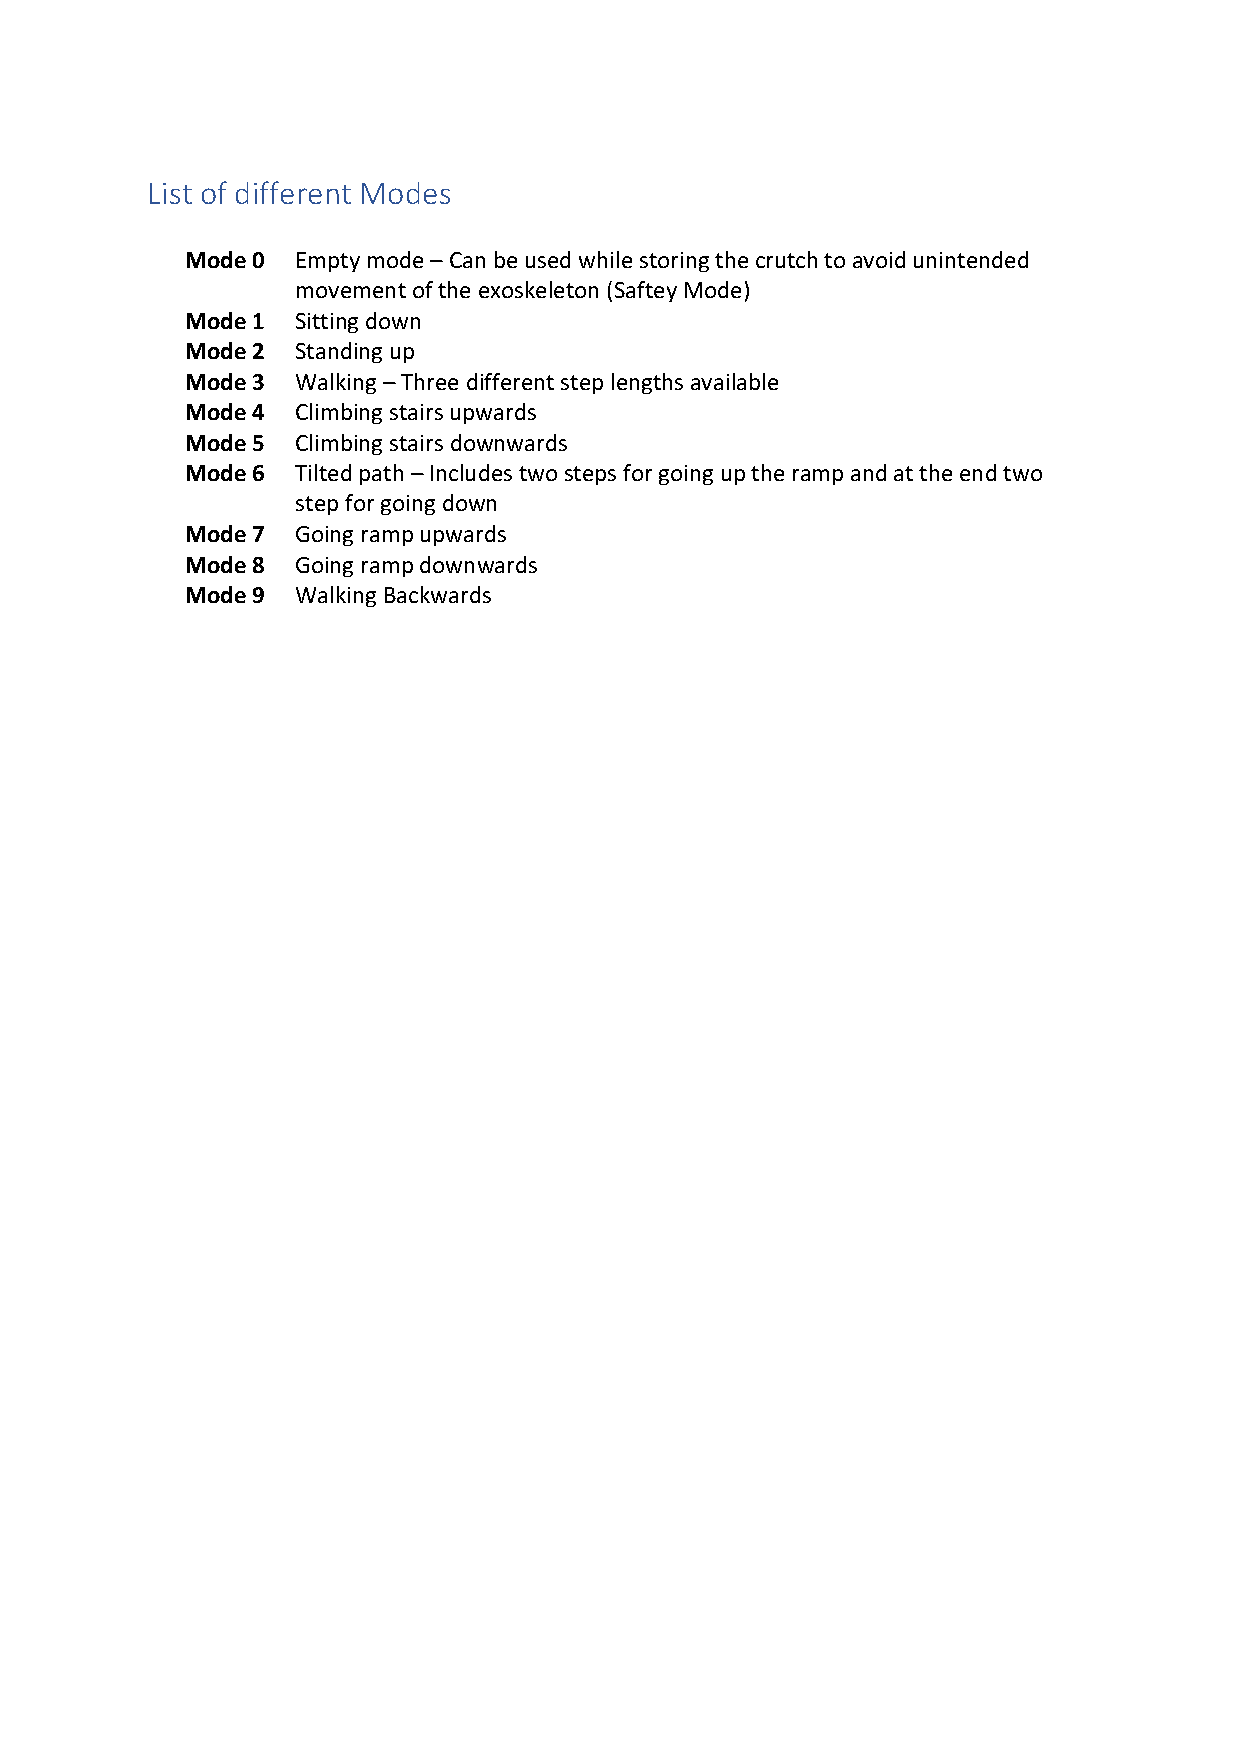
\includepdf[pages=1]{Appendix/ergonomic_crutch/List_of_different_Modes.pdf}
\label{subsec:list of modes}


\begin{enumerate}[ii.]
\item{Length Adjustment Mechanism}
\end{enumerate}
\label{subsec:LAM}

The length adjustment mechanism had to fulfill many requirements, none of the commercial state-of-the-art solutions fulfilled all the requirments; therefore, a new solution was developed.\\
\begin{figure}
    \centering
    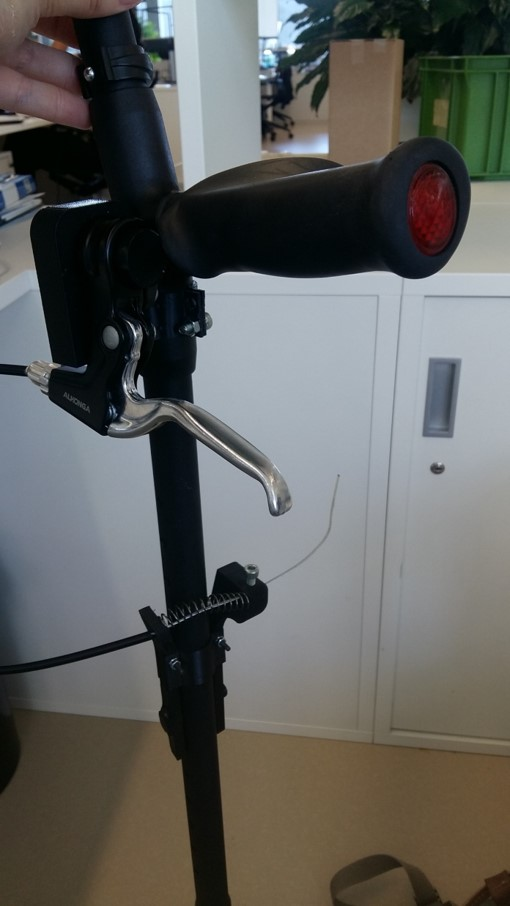
\includegraphics[width=0.8\columnwidth]{Appendix/LAM/3D_prototype_LAM.jpg}
    \caption{The length adjustment mechanism was iteratively designed with 3D prototypes}
    \label{fig:3D_LAM}
\end{figure}
\begin{figure}
    \centering
    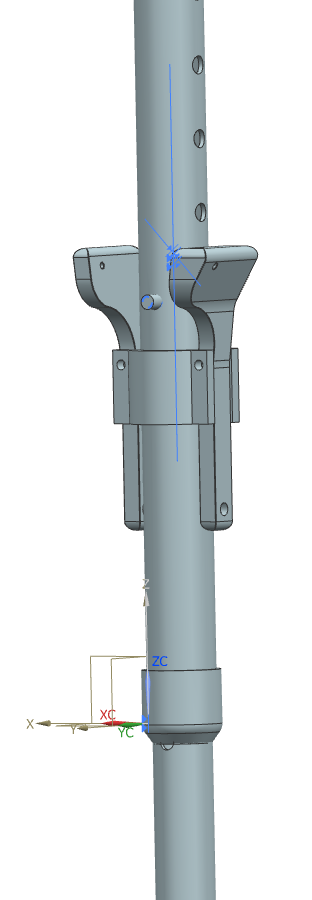
\includegraphics[width=0.8\columnwidth]{Appendix/LAM/Zangenassembly.png}
    \caption{The clamp mechanism was designed in CAD.}
    \label{fig:CAD_LAM}
\end{figure}
\begin{figure}
    \centering
    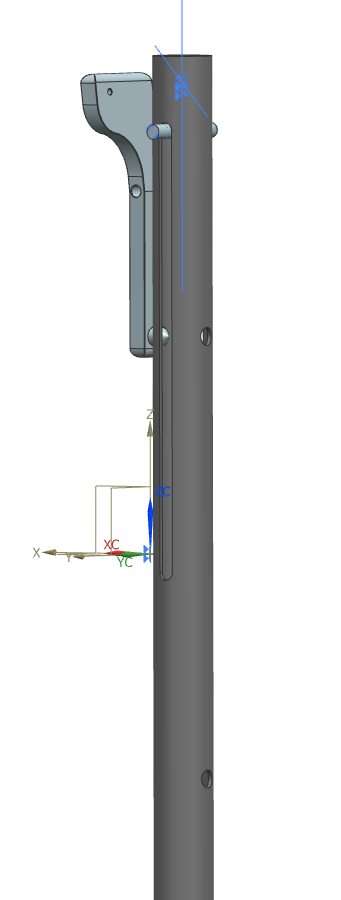
\includegraphics[width=0.8\columnwidth]{Appendix/LAM/bottom_crutch.png}
    \caption{\textbt{The bottom pipe of the crutch:} The bottom part has a slot where a pin can slide along, the feature fulfills two main requirements. The pin indicates the end positions and helps finding the right position for the clamp to snap in. Additionally, the pin prevents the two crutch pipes from turning relative to each other, which would prevent the clamp from snapping in.}
    \label{fig:pin_LAM}
\end{figure}

The mechanism seems very promising, the position of the shoulders of the pilot sitting is more comfortable see fig.\ref{fig:shoulderup} and fig.\ref{fig:shoulderdown}. The pilot can also keep an upright posture despite of uneven grounds, see fig.\ref{fig:tilted}.

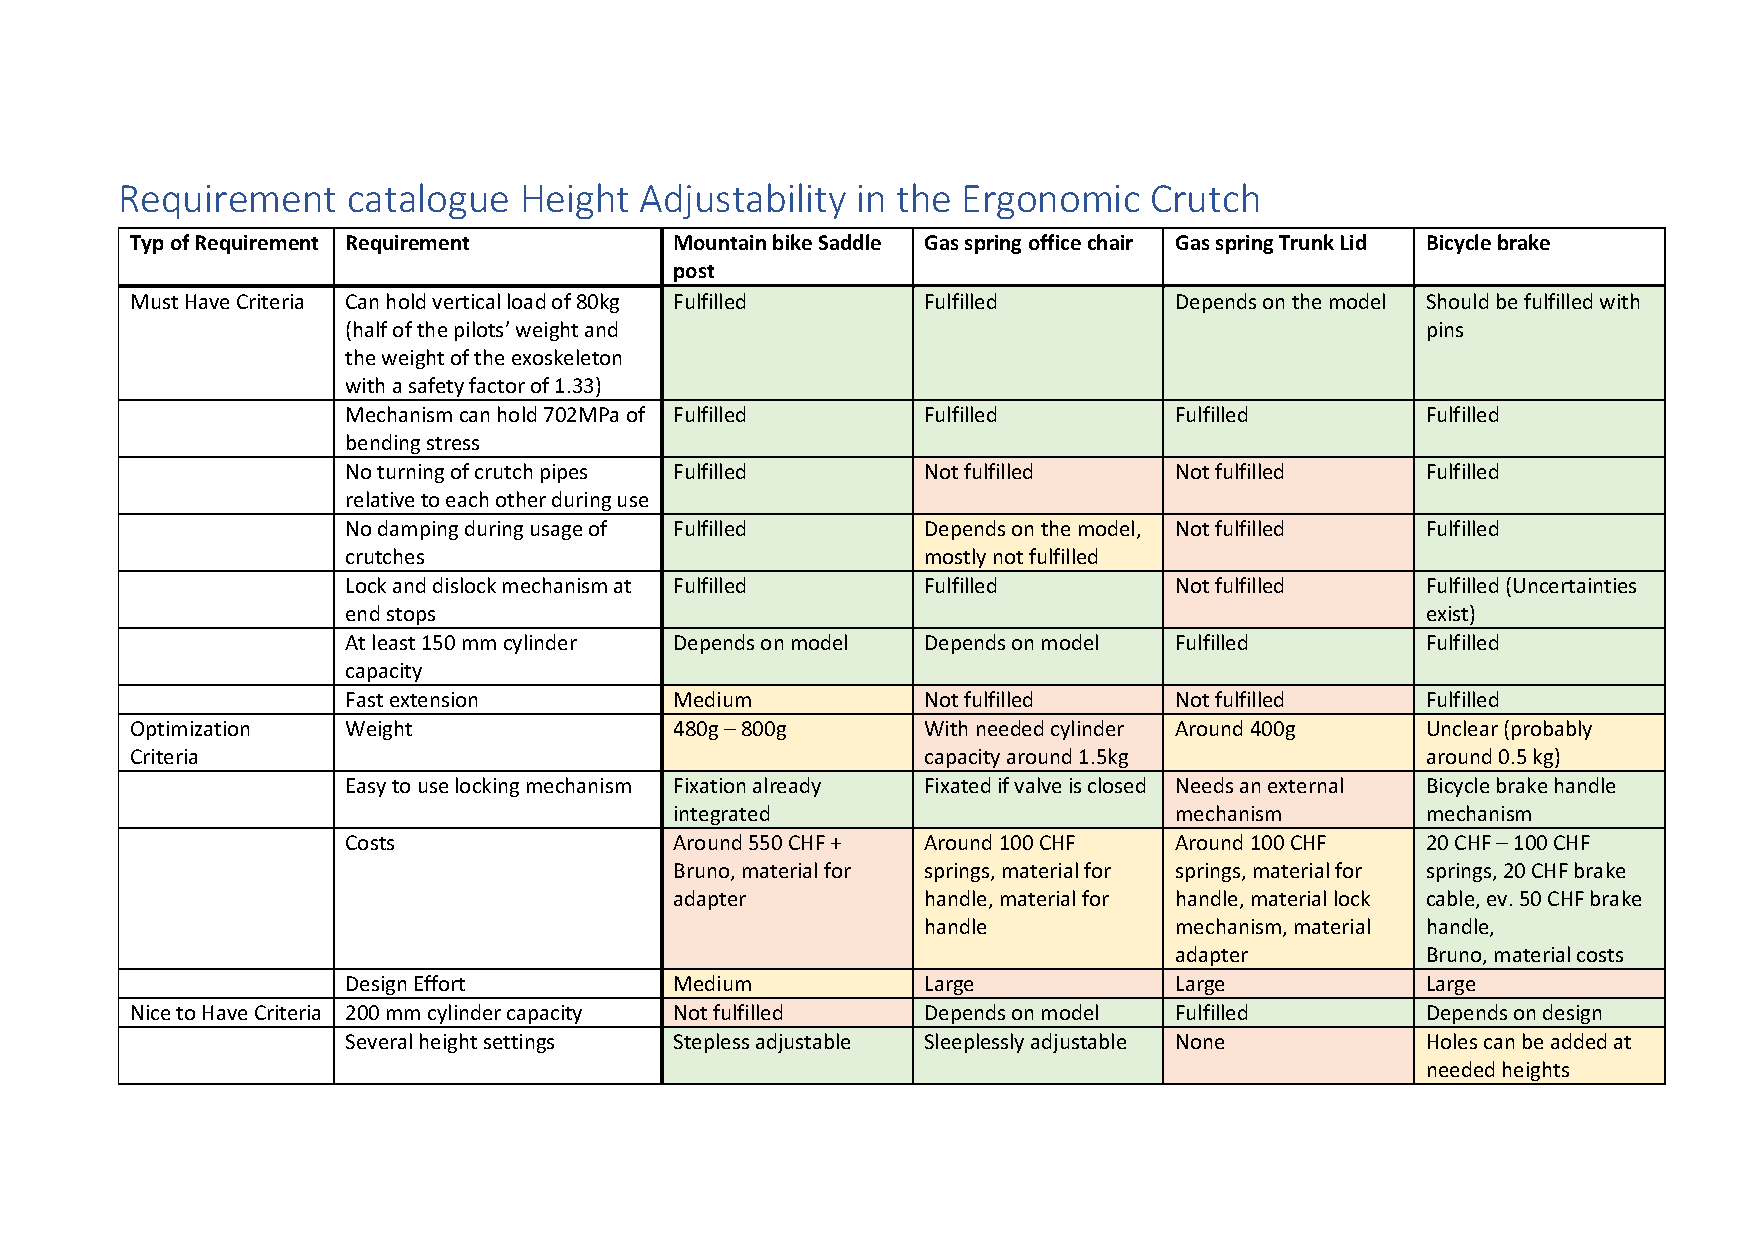
\includepdf[pages=1]{Appendix/LAM/requirements_LAM.pdf}
\label{pdf:requirementsLAM}
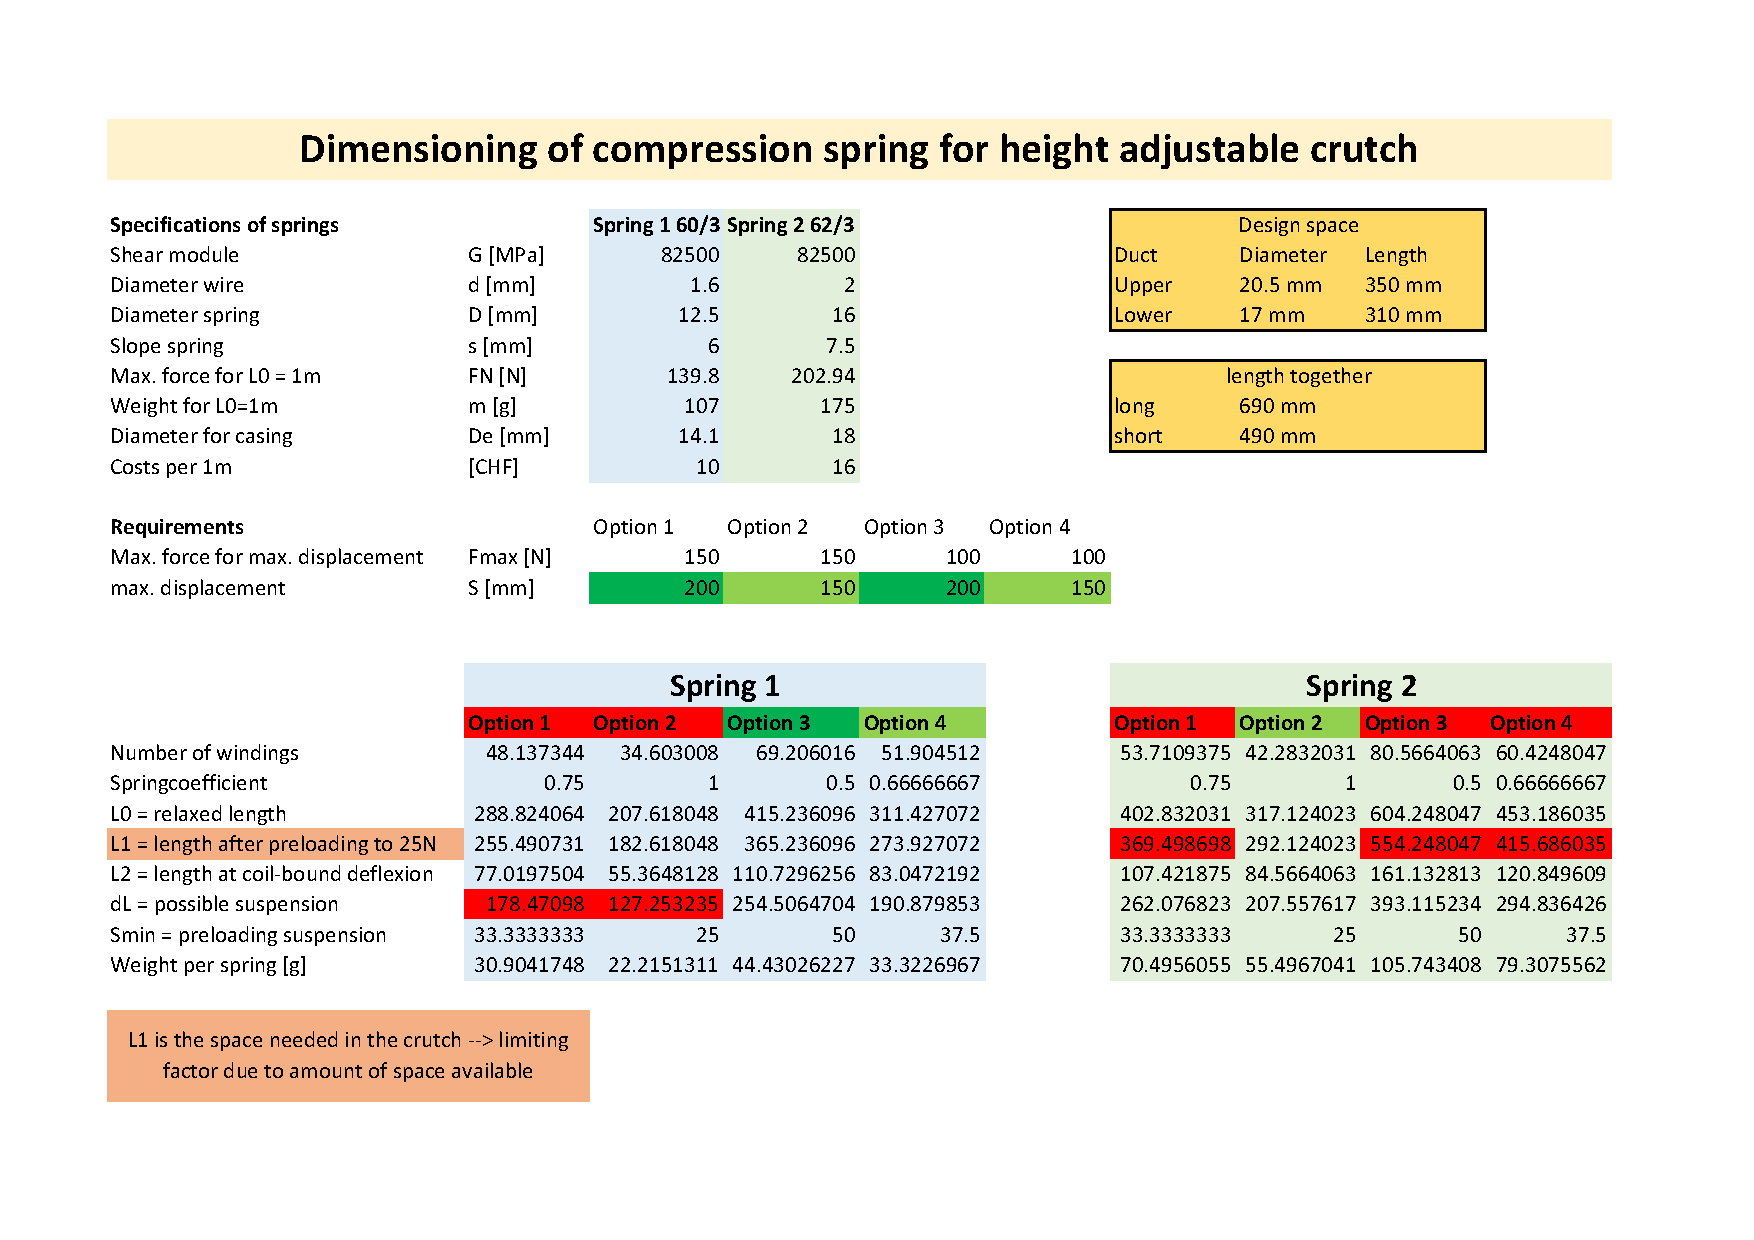
\includepdf[pages=1]{Appendix/LAM/Auslegung_Druckfeder_V2.pdf}
\label{pdf:spring}



\begin{figure}
    \centering
    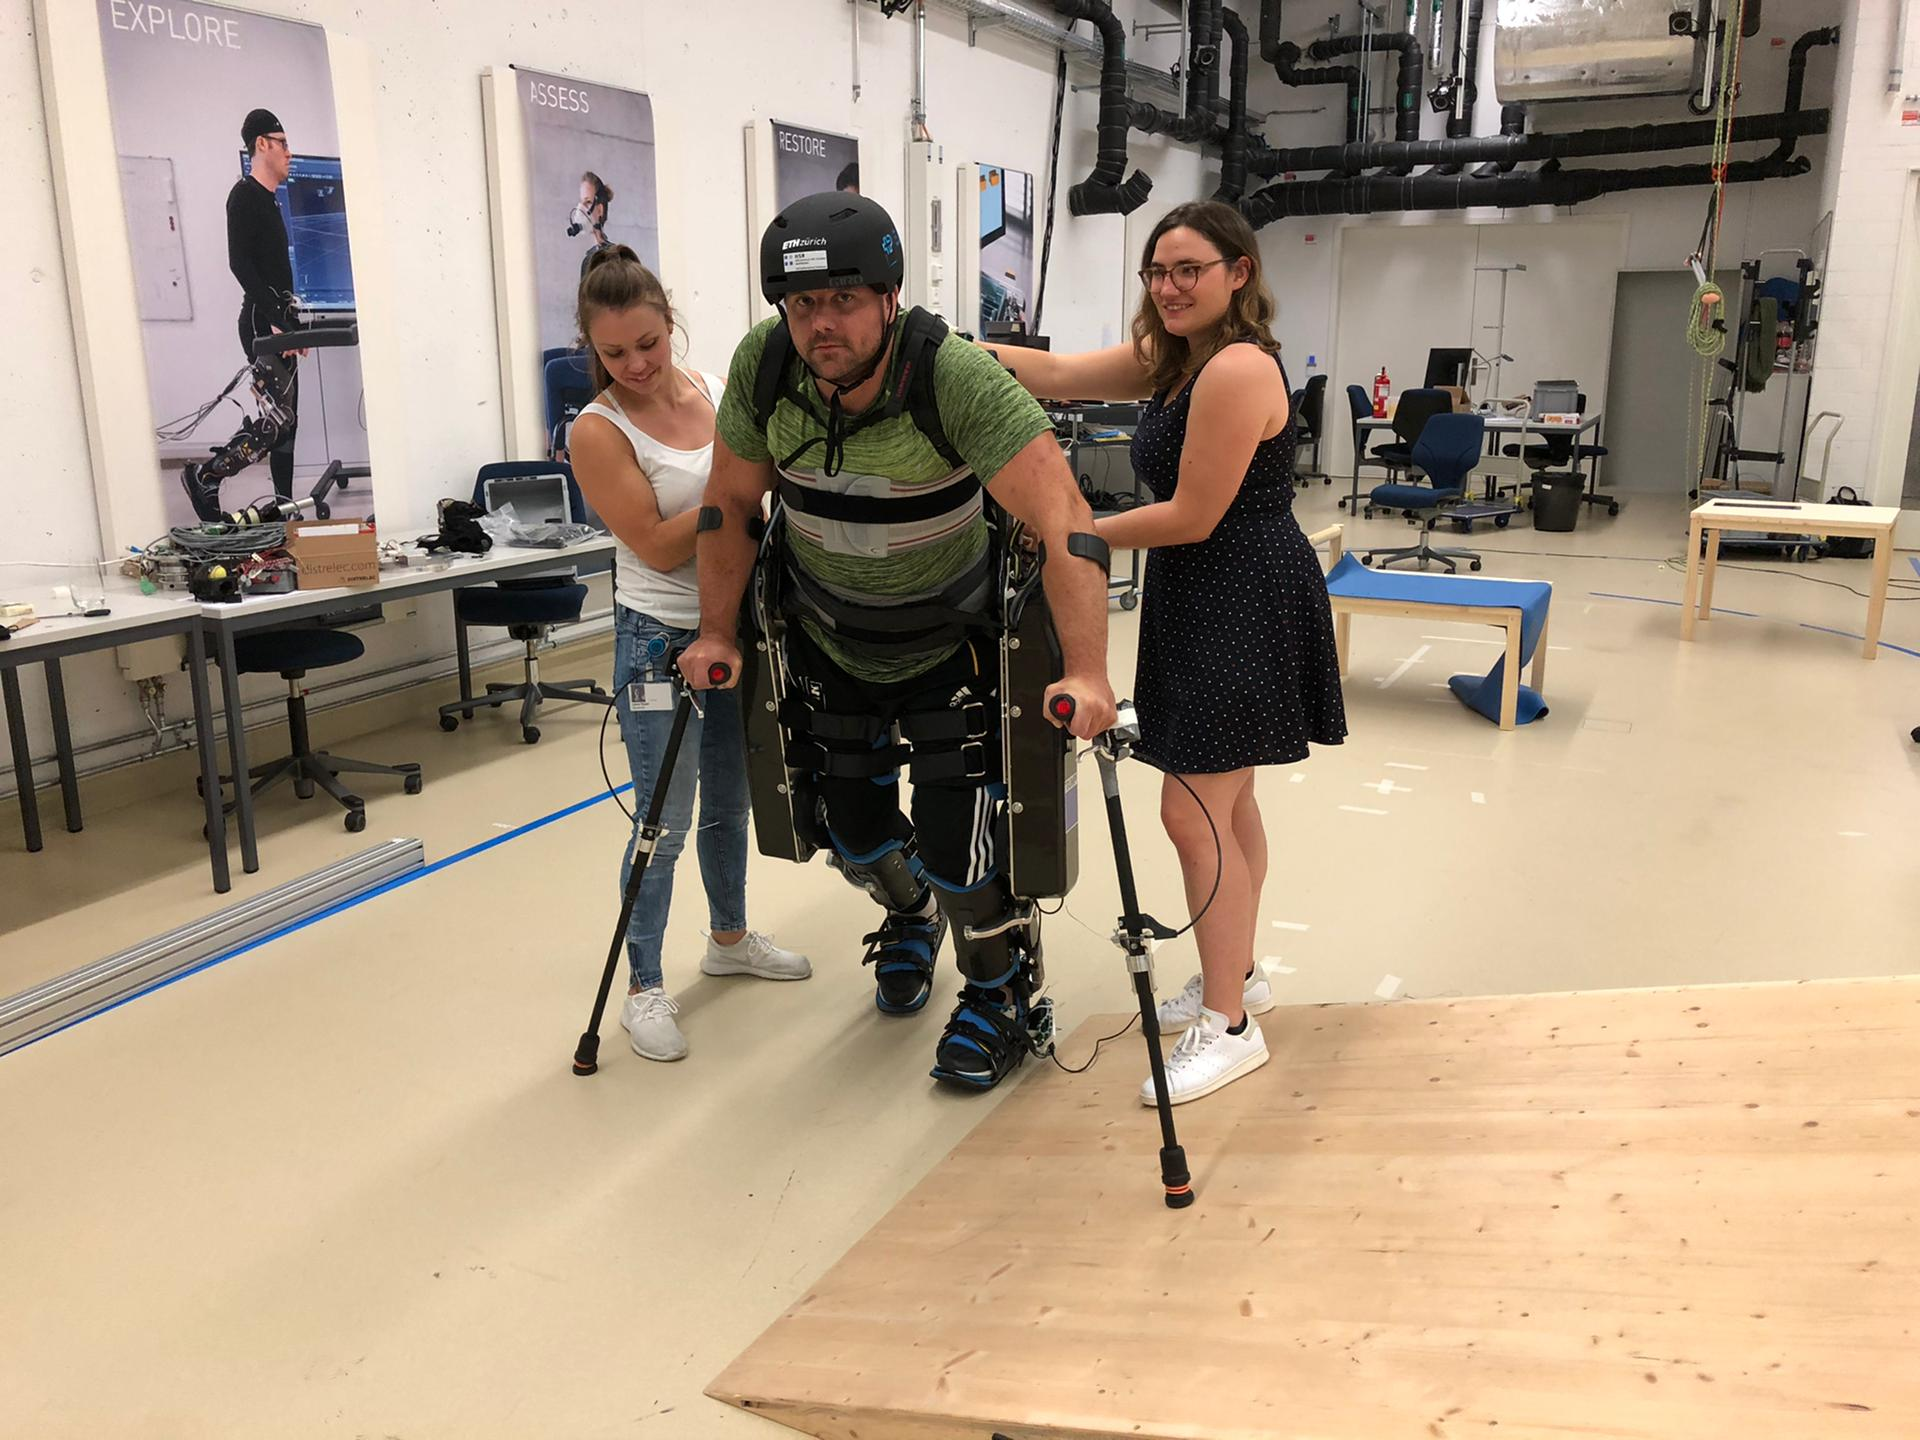
\includegraphics[width=1\columnwidth]{Appendix/LAM/tiltedpath.jpeg}
    \caption{The shortened crutch helps the pilot to stand upright on a tilted path despite the difference in height of the ground below the crutches.}
    \label{fig:tilted}
\end{figure}

\begin{figure}
    \centering
    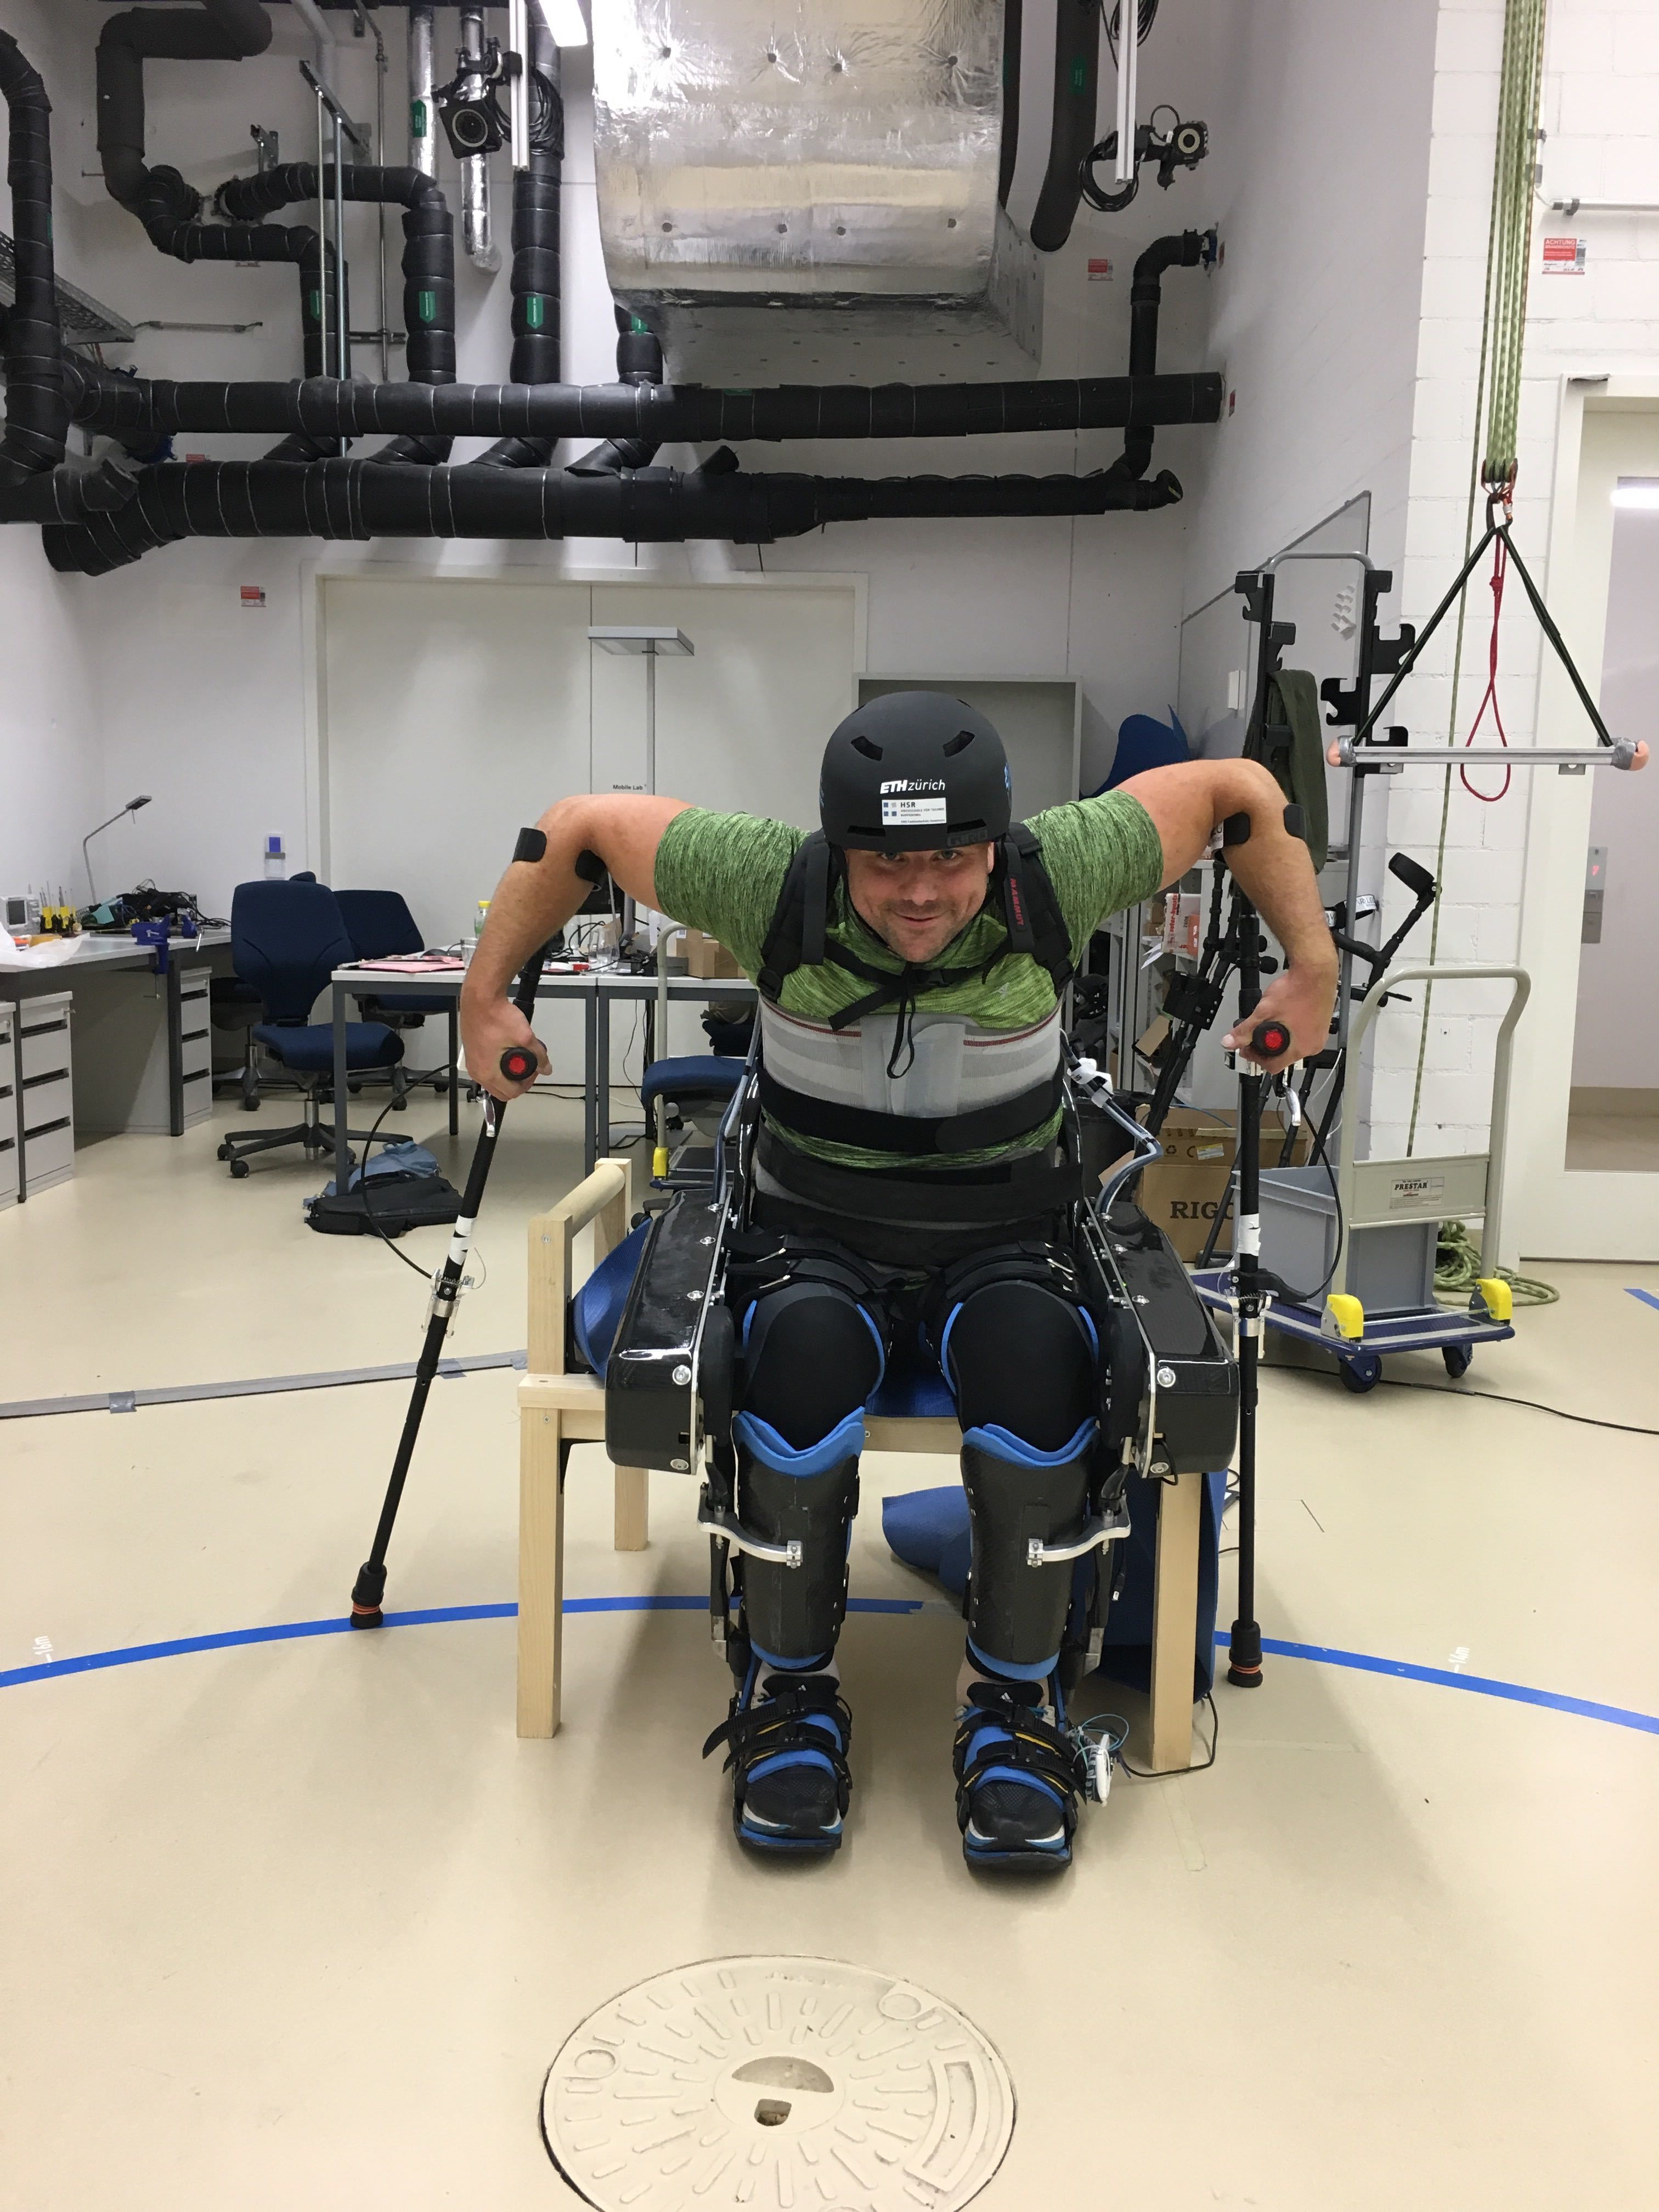
\includegraphics[width=0.8\columnwidth]{Appendix/LAM/shouldersup.JPG}
    \caption{The length adjustment mechanism was iteratively designed with 3D prototypes}
    \label{fig:shoulderup}
\end{figure}

\begin{figure}
    \centering
    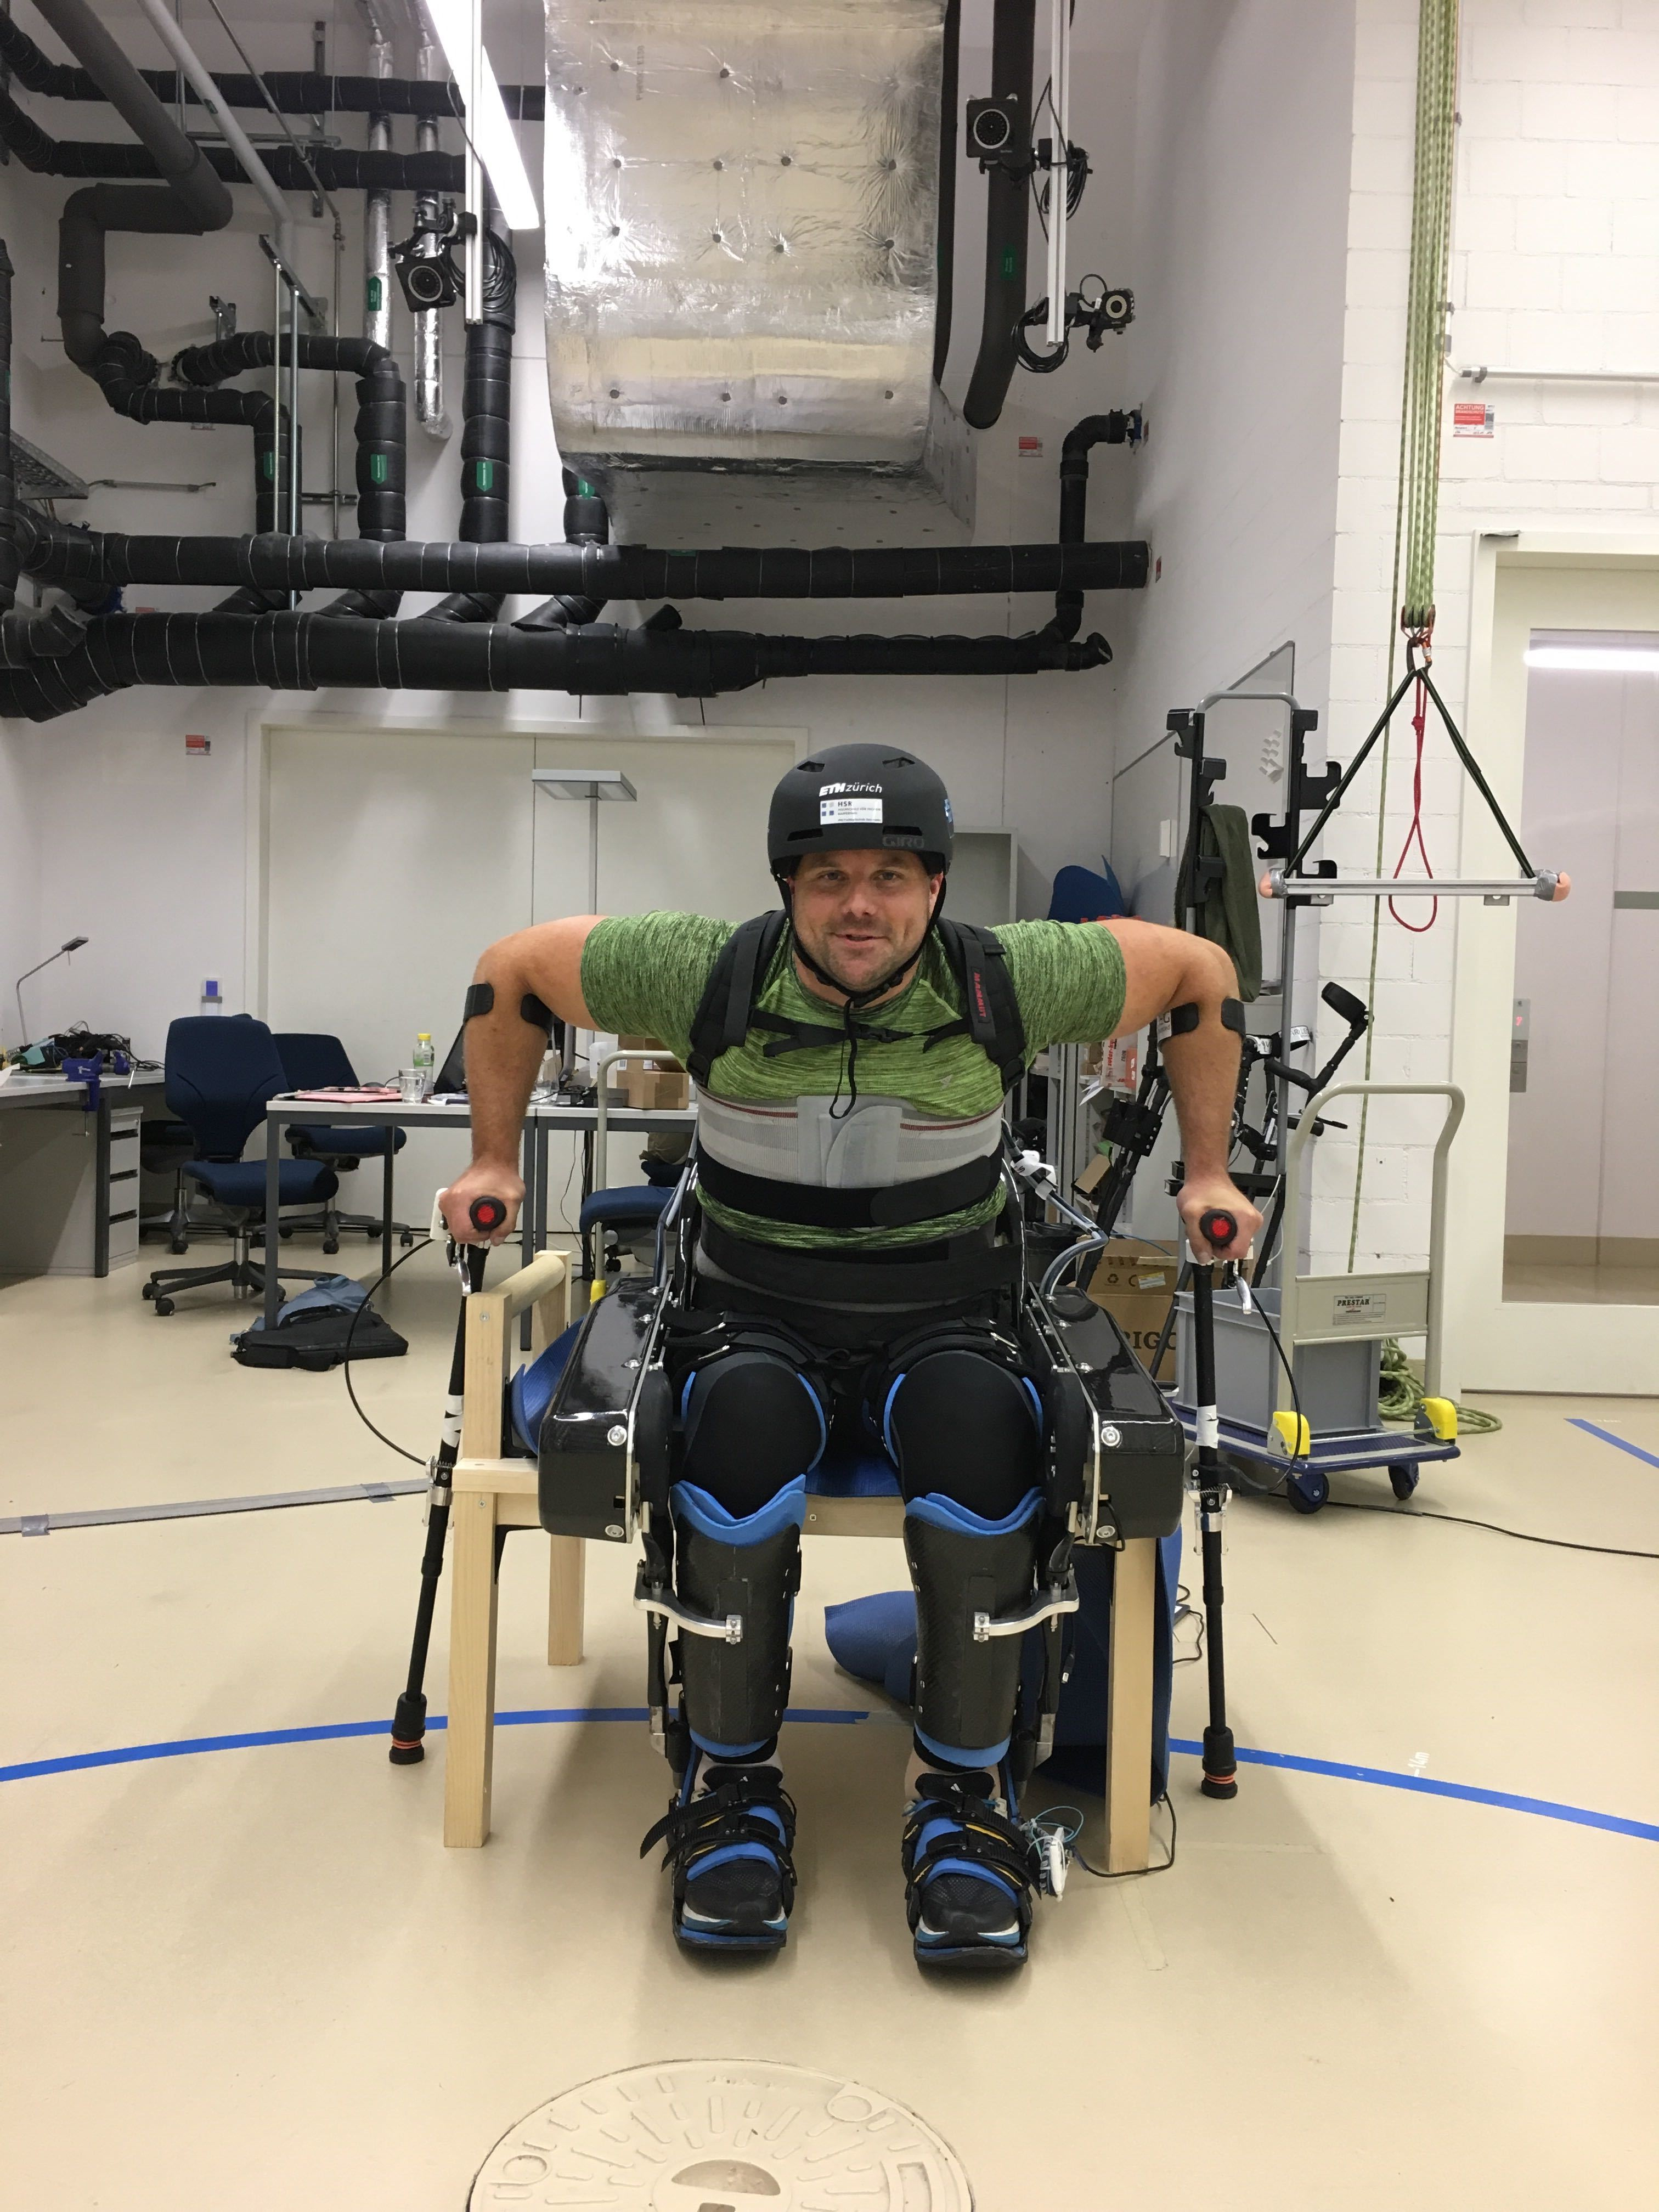
\includegraphics[width=0.8\columnwidth]{Appendix/LAM/shouldersdown.JPG}
    \caption{The length adjustment mechanism was iteratively designed with 3D prototypes}
    \label{fig:shoulderdown}
\end{figure}


%%%%%%%%%%%%%%%%%%%%%%%%%%%%%%%%%%%%%%%%%%%%%%%%%%%%%%%%%%%%%%%%%%%%%%%%%%%%%%%%%%%%%%%
\cleardoublepage
\begin{enumerate}[iii.]
\item{Haptic Feedback} 
\end{enumerate}

%%%%%% HF requirements

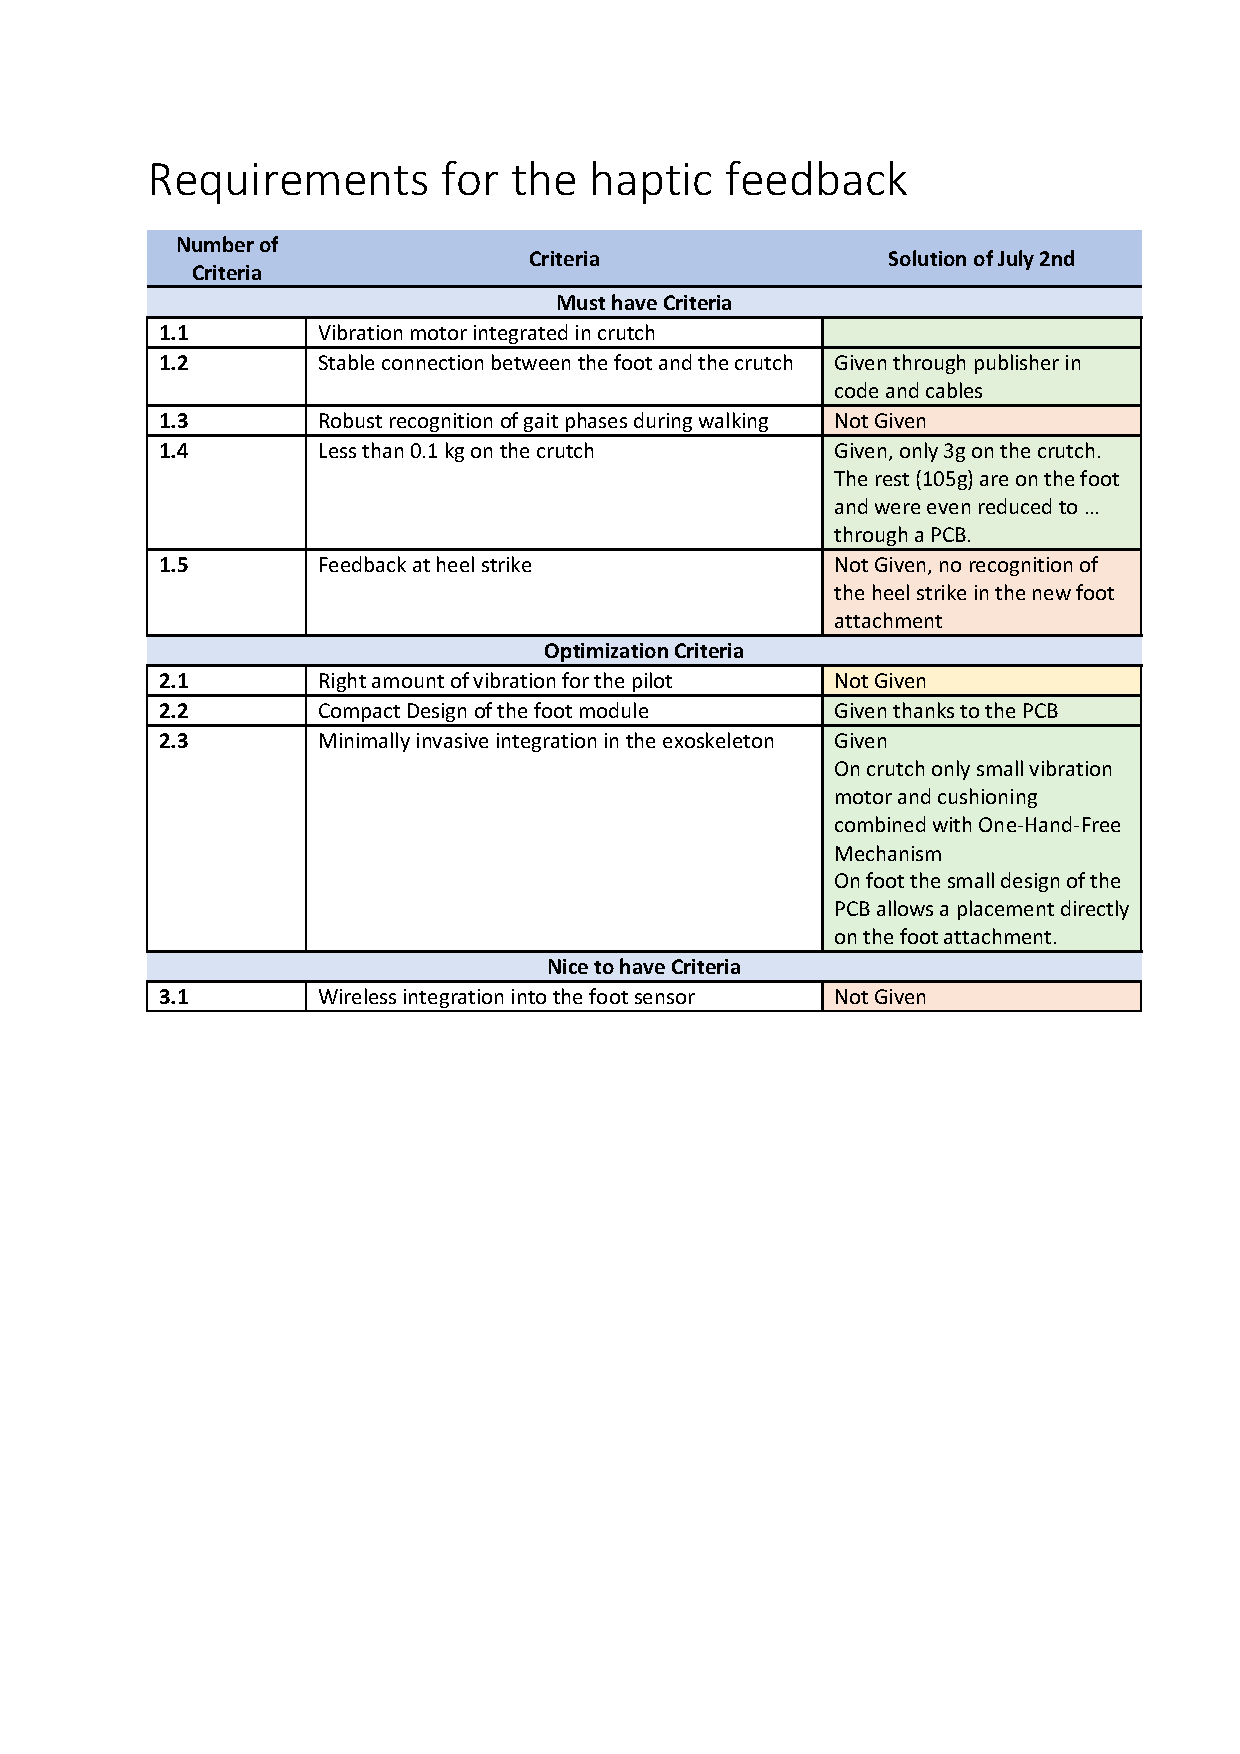
\includepdf[pages=1]{Appendix/haptic_feedback/requirements_haptic_feedback.pdf}
\label{subsec:HF requirements}
%%%%%% HF Empathize

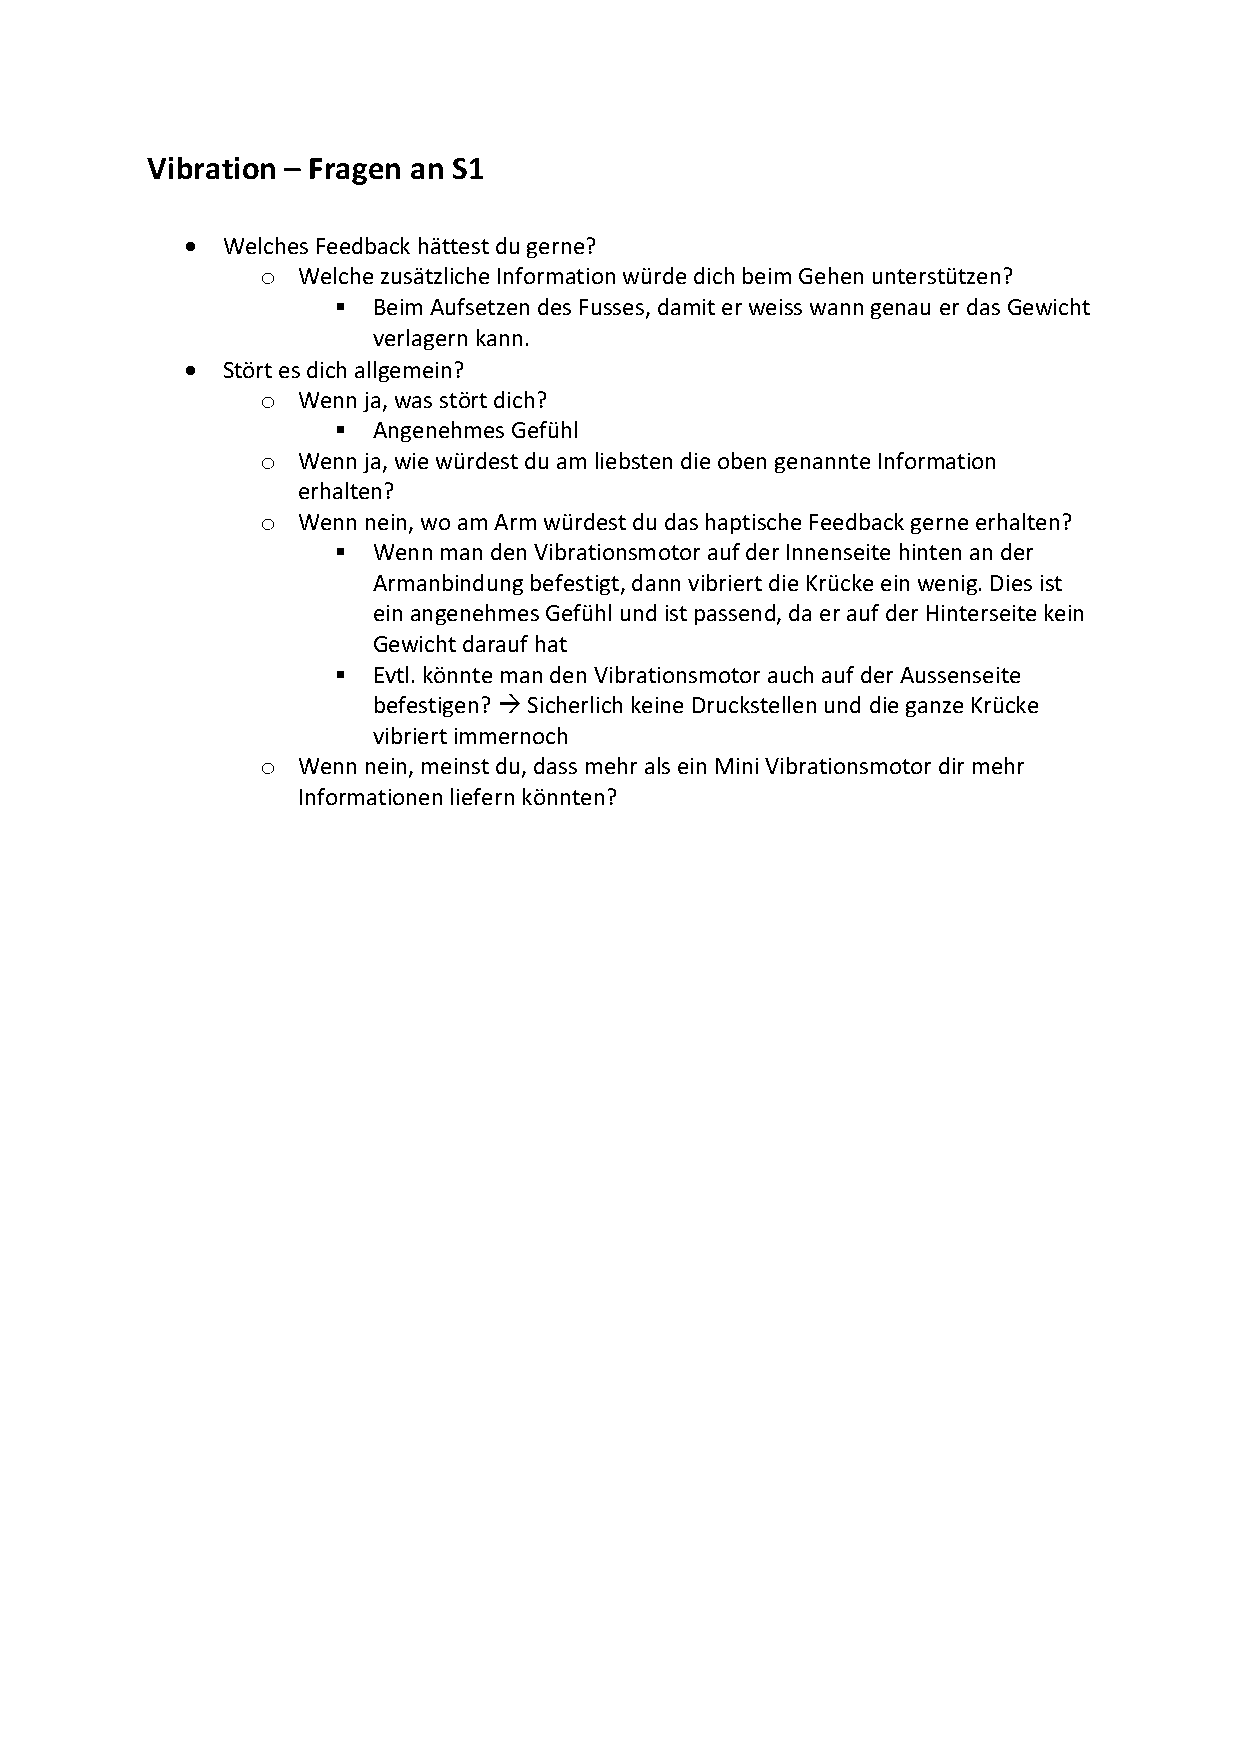
\includepdf[pages=1]{Appendix/haptic_feedback/Fragen_Thomas_Haptisches_Feedback.pdf}
\label{subsec:HF Vibration}

%%%%%% Schematics of the PCB


\begin{figure}
    \centering
    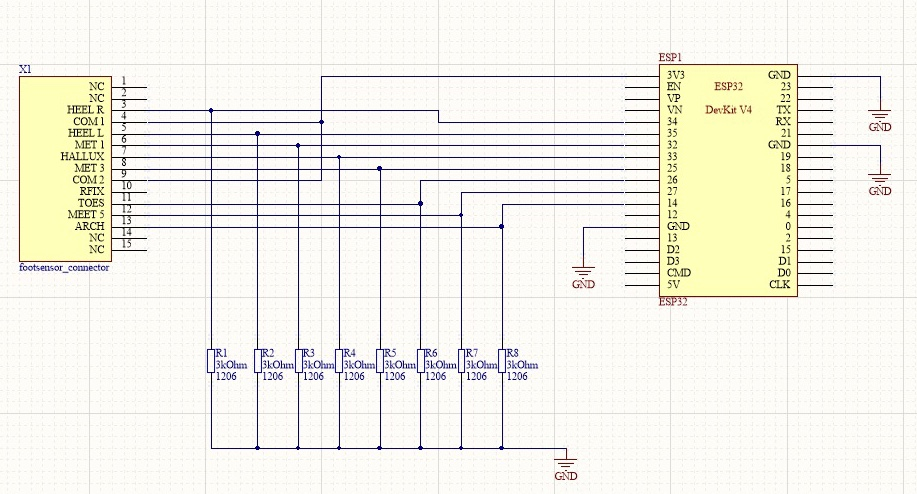
\includegraphics[width=1\columnwidth]{Appendix/haptic_feedback/Schematics.jpg}
    \caption{\textbf{Schematics of the foot sensor PCB:} The following schematics was used to implement the IEE foot pressure insole in combination witht the ESP32 DevKit V4}
    \label{fig:schematics}
\end{figure}

%%%%%% Integration of the Vibration Motor

\begin{figure}[!t]
	\centering
	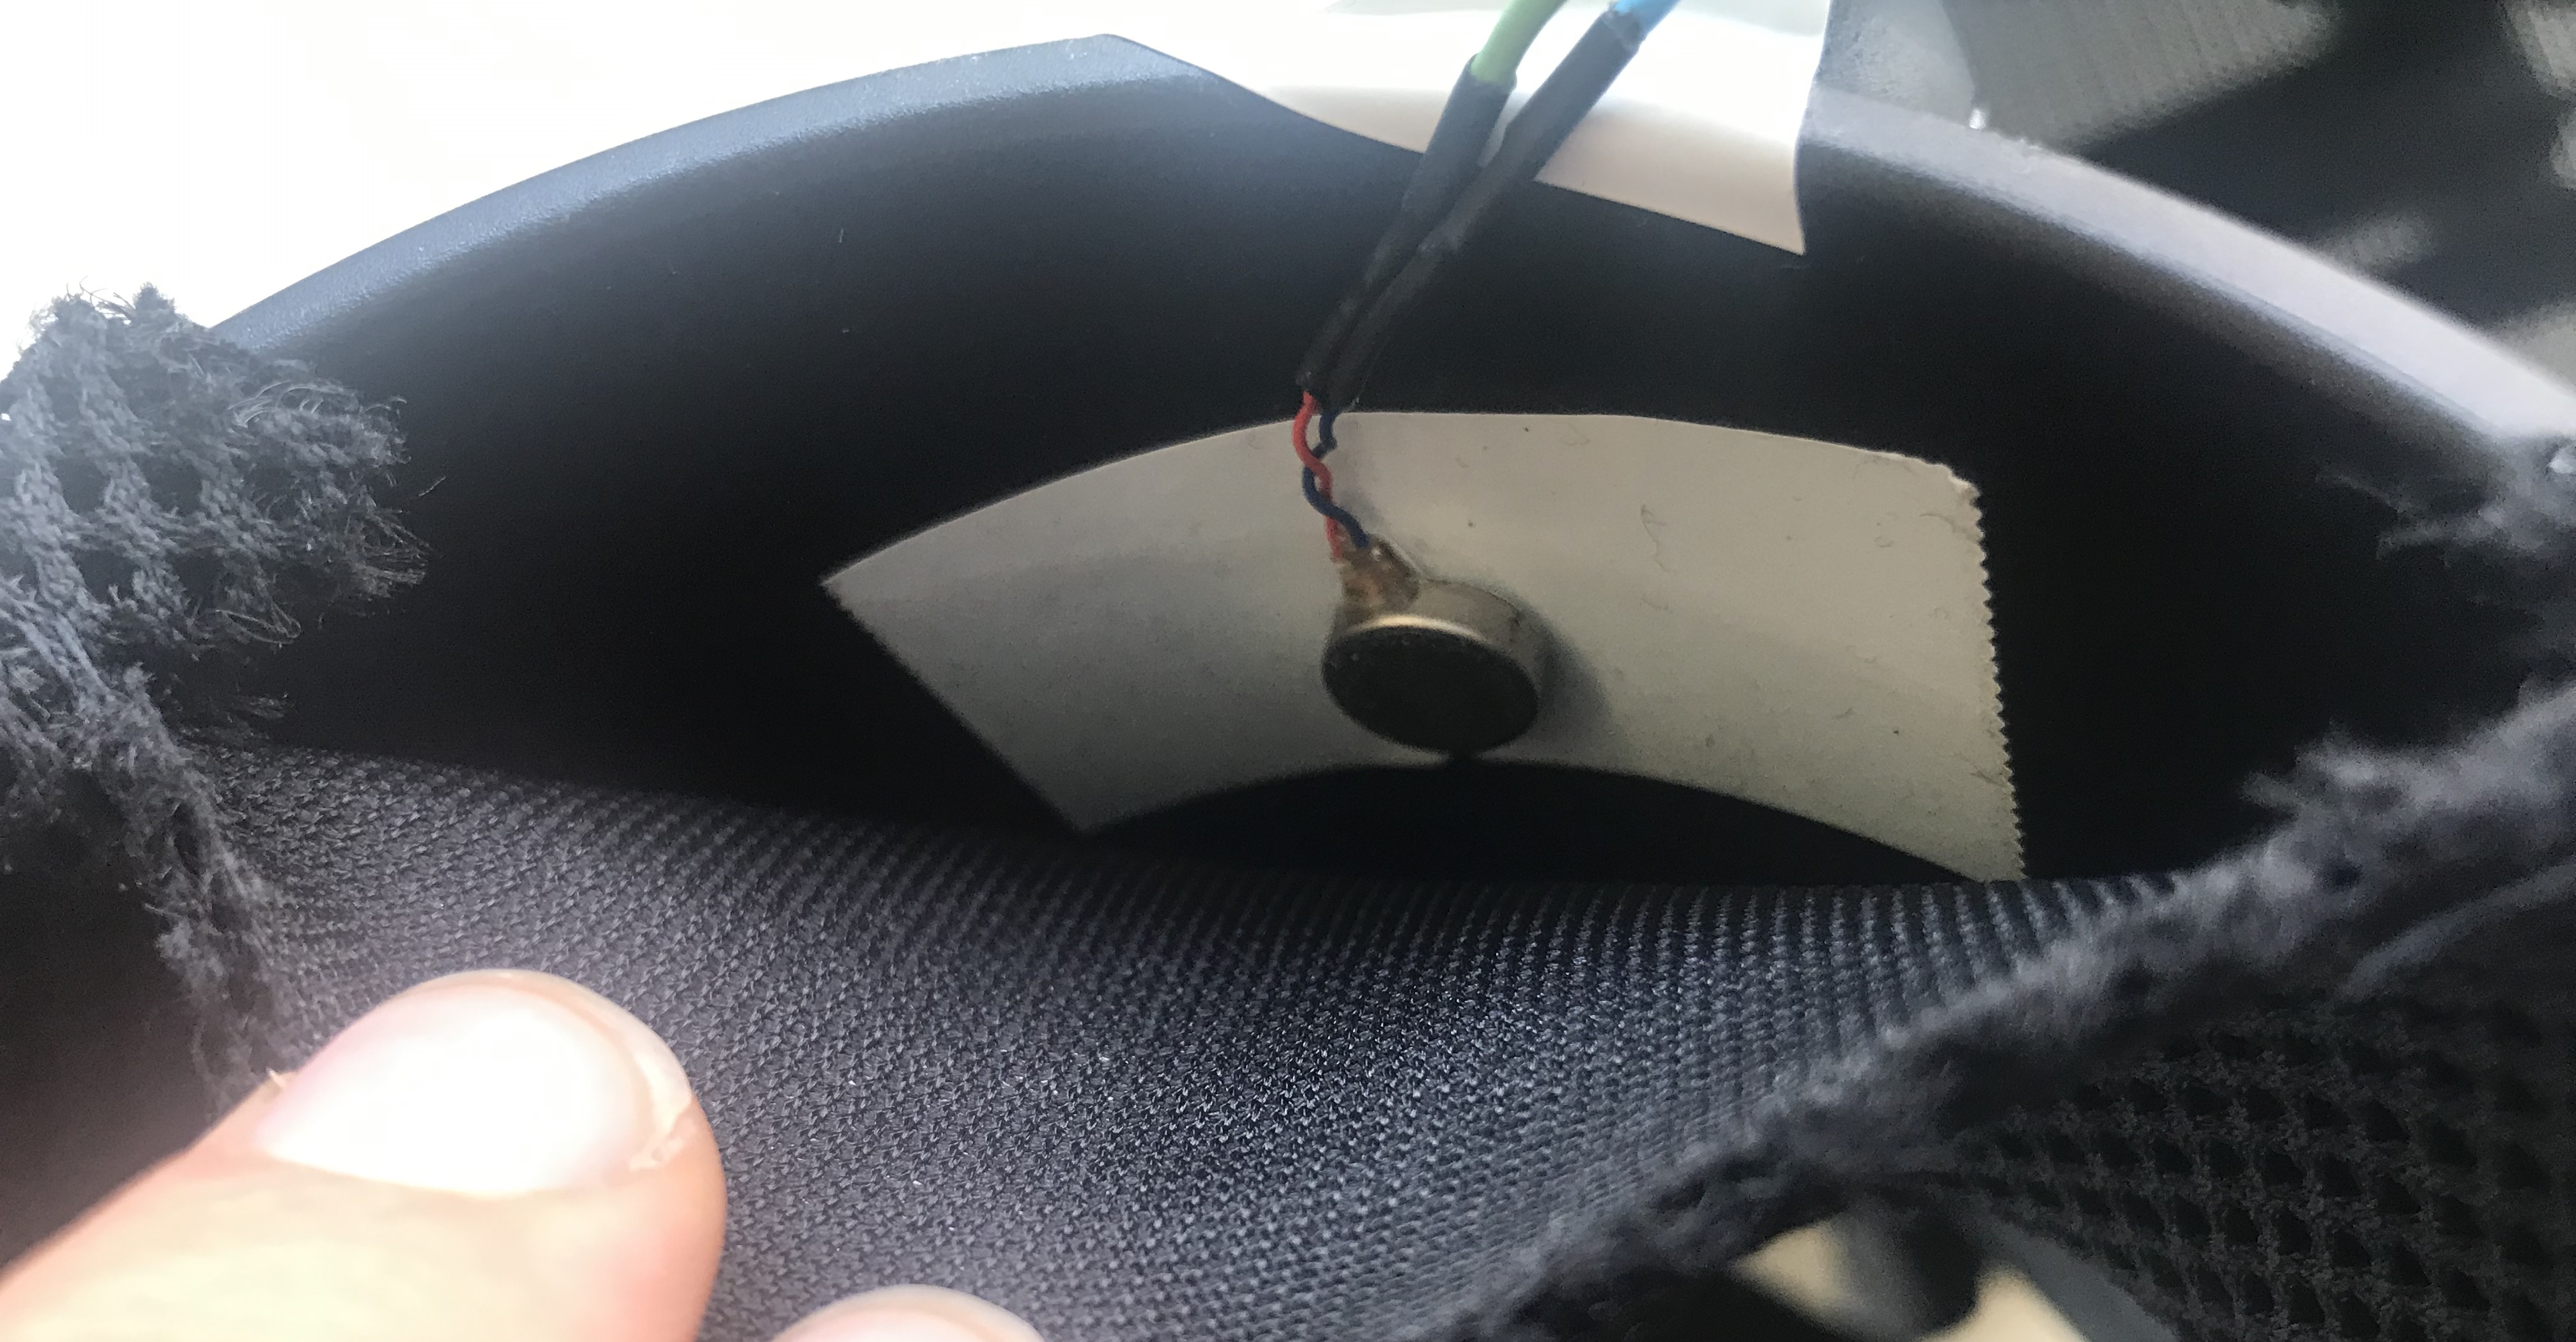
\includegraphics[width=1\columnwidth]{Appendix/haptic_feedback/Vibration.jpg}
	\caption{\textbf{Flat Coin Vibration Motor on the inside of the closed cuff}}
	\label{fig: vibration}
\end{figure}


%%%%%% Foot Sensor Placement – Inside the shoe

\begin{figure}[!t]
	\centering
	\includegraphics[width=1\columnwidth]{Appendix/haptic_feedback/Placement_in_Shoe.jpg}
	\caption{\textbf{Placement inside the shoe:} The foot pressure sensor was placed inside the shoe between the inner sole and the outer sole.}
	\label{fig: inside shoe}
\end{figure}

%%%%%% Foot Sensor Placement – Outside the shoe

\begin{figure}[!t]
	\centering
	\includegraphics[width=1\columnwidth]{Appendix/haptic_feedback/Placement_outside_shoe.jpg}
	\caption{\textbf{Placement outside the shoe:} The foot pressure sensor was placed outside the shoe between the outer sole and a self-made sock to avoid the sole from being slippery.}
	\label{fig: oudside shoe}
\end{figure}

%%%%%% Foot Sensor Placement – New shoe attachment

\begin{figure}[!t]
	\centering
	\includegraphics[width=1\columnwidth]{Appendix/haptic_feedback/Aussensohle.JPG}
	\caption{\textbf{New shoe attachment of the VariLeg enhanced exoskeleton:} The soles can be placed on the inside of the new shoe attachment between the pilot's shoe and the new shoe attachment.}
	\label{fig: new shoe attachment}
\end{figure}

%%%%%% Paddings

\begin{figure}[!t]
	\centering
	\includegraphics[width=1\columnwidth]{Appendix/haptic_feedback/Aussensohle.JPG}
	\caption{\textbf{Paddings:} Paddings out of self-adhesive neoprene material was placed on each cell to make sure the force flux runs through the cells. Unfortunately, this led to inner stresses due to bending of the unflexible material.}
	\label{fig: paddings}
\end{figure}

%%%%%% Arduino Nano

\begin{figure}[!t]
	\centering
	\includegraphics[width=1\columnwidth]{Appendix/haptic_feedback/Setup_mit_arduino.png}
	\caption{\textbf{Initial Setup with a prototype PCB and an Arduino Nano }}
	\label{fig: Arduino Nano}
\end{figure}

%%%%%% PCB selfmade

\begin{figure}[!t]
	\centering
	\includegraphics[width=1\columnwidth]{Appendix/haptic_feedback/handgemachtes_PCB_offen.JPG}
	\caption{\textbf{Prototype PCB}}
	\label{fig: PCB selfmade}
\end{figure}

%%%%%% PCB selfmade

\begin{figure}[!t]
	\centering
	\includegraphics[width=1\columnwidth]{Appendix/haptic_feedback/PCB.JPG}
	\caption{\textbf{Designed PCB:}  This PCB allows the implementation of the foot module compactly in combination with the ESP32 DevKit V4.}
	\label{fig: PCB selfmade}
\end{figure}

%%%%%% Calibration of foot sensor


\begin{table}[!t]
	\renewcommand{\arraystretch}{1.3}
% if using array.sty, it might be a good idea to tweak the value of \extrarowheight as needed to properly center the text within the cells
	\caption{Data of the calibration of the IEE foot sensor by applying aroung 5kg to each sensor cell}
	\label{tab: calibration}
	\centering
% Some packages, such as MDW tools, offer better commands for making tables
% than the plain LaTeX2e tabular which is used here.
		\begin{tabular}{l|ccc}
			\hline
			Sensor Cell Position & Mean [V] & Standard Deviation [V] \\ \hline 
			Heel R  & 0.556 & 0.026  \\
			Heel L  & 0.449 & 0.026  \\
		    Arch & 0.516 & 0.022 \\
			Met 1 & 0.551 & 0.025  \\
			Met 3 & 0.567 & 0.050  \\
			Met 5 & 0.627 & 0.024  \\
		    Hallux & 0.476 & 0.053  \\		    	Toes & 0.466 & 0.029  \\

			\hline
		\end{tabular}
\end{table}

\cleardoublepage
\begin{enumerate}[iv.]
\item{Datasheets} 
\end{enumerate}
%%%%%% Datasheet ESP


\includepdf[pages={1,2,3,4,5,6,7,8,9,10}]{Appendix/haptic_feedback/Datasheet_ESP.pdf}
\label{subsec:HF ESP}

%%%%%% HF Datasheet Insole

\includepdf[page={1,2,3,4,5,6,7,8,9}]{Appendix/haptic_feedback/Datasheet_Insole.pdf}
\label{subsec:HF Insole}

%%%%%% HF Datasheet Flat Coin Vibration Motor


\includepdf[pages={1,2,3,4,5,6,7,8,9,10}]{Appendix/haptic_feedback/Flat_coin_vibration_motor.pdf}
\label{subsec:HF ESP}



%%*************************************************************************

%BEGIN{RELAB} :: optional datasheets and other pdf documents
%\cleardoublepage
%\includepdf[pages={1,3,4-5},angle=0,nup=2x2,frame=true, scale=0.9]{Appendix/PicDatasheet.pdf}
%\includepdf[pages=1]{Appendix/SharpDatasheet.pdf}

%END{RELAB} 

%%*************************************************************************
%\input{Appendix text files/1_User-cenered_Design_Method.tex}
%\input{Appendix text files/2_Ergonomic_Design.tex}
%\input{Appendix text files/3_Length_adjustment.tex}
%\input{Appendix text files/4_Haptic_Feedback.tex}
%END{RELAB} 

%%*************************************************************************

% that's all folks


%%*************************************************************************
\end{document}


